%%%%%%%%%%%%%%%%%%%%%%%%%%%%%%%%%%%%%%%%%%%%%%%%%%%%%%%%%%%%%%%%%%%%%%%%%%%%%%%%
%% Plantilla de memoria en LaTeX para la ETSIT - Universidad Rey Juan Carlos
%%
%% Por Gregorio Robles <grex arroba gsyc.urjc.es>
%%     Grupo de Sistemas y Comunicaciones
%%     Escuela Técnica Superior de Ingenieros de Telecomunicación
%%     Universidad Rey Juan Carlos
%% (muchas ideas tomadas de Internet, colegas del GSyC, antiguos alumnos...
%%  etc. Muchas gracias a todos)
%%
%% La última versión de esta plantilla está siempre disponible en:
%%     https://github.com/gregoriorobles/plantilla-memoria
%%
%% Para obtener PDF, ejecuta en la shell:
%%   make
%% (las imágenes deben ir en PNG o JPG)

%%%%%%%%%%%%%%%%%%%%%%%%%%%%%%%%%%%%%%%%%%%%%%%%%%%%%%%%%%%%%%%%%%%%%%%%%%%%%%%%

\documentclass[a4paper, 12pt]{book}
%\usepackage[T1]{fontenc}

\usepackage[a4paper, left=2.5cm, right=2.5cm, top=3cm, bottom=3cm]{geometry}
\usepackage{times}
\usepackage[utf8]{inputenc}
\usepackage[spanish]{babel} % Comenta esta línea si tu memoria es en inglés
\usepackage{url}
%\usepackage[dvipdfm]{graphicx}
\usepackage{graphicx}
\usepackage{float}  %% H para posicionar figuras
\usepackage[nottoc, notlot, notlof, notindex]{tocbibind} %% Opciones de índice
\usepackage{latexsym}  %% Logo LaTeX

\usepackage{listings}
\usepackage{color}

% Para mostrar código
\definecolor{dkgreen}{rgb}{0,0.6,0}
\definecolor{gray}{rgb}{0.5,0.5,0.5}
\definecolor{mauve}{rgb}{0.58,0,0.82}

\lstset{frame=tb,
  language=XML,
  aboveskip=3mm,
  belowskip=3mm,
  showstringspaces=false,
  columns=flexible,
  basicstyle={\tiny\ttfamily},
  numbers=none,
  numberstyle=\tiny\color{gray},
  keywordstyle=\color{blue},
  commentstyle=\color{dkgreen},
  stringstyle=\color{mauve},
  breaklines=true,
  breakatwhitespace=true,
  tabsize=3
}
%%%%%%%%%%%%%%%%%%%%%%%%%%%%

\title{Memoria del Proyecto}
\author{Daniel Hervás Rodao}

\renewcommand{\baselinestretch}{1.5}  %% Interlineado

\begin{document}

\renewcommand{\refname}{Bibliografía}  %% Renombrando
\renewcommand{\appendixname}{Apéndice}

%%%%%%%%%%%%%%%%%%%%%%%%%%%%%%%%%%%%%%%%%%%%%%%%%%%%%%%%%%%%%%%%%%%%%%%%%%%%%%%%
% PORTADA

\begin{titlepage}
\begin{center}

\includegraphics[scale=0.8]{img/URJ_logo_Color_POS.png}

\vspace{1.75cm}

\Large
GRADO EN INGENIERÍA EN TELEMÁTICA

\vspace{0.4cm}

\large
Curso Académico 2021/2022

\vspace{0.8cm}

Trabajo Fin de Grado

\vspace{2.5cm}

\LARGE
GAMIFICACIÓN DE PLATAFORMA UNIBOTICS

\vspace{4cm}

\large
Autor : Daniel Hervás Rodao \\
Tutor : José María Cañas Plaza \\
Co-Tutor : David Roldán Álvarez
\end{center}
\end{titlepage}

\newpage
\mbox{}
\thispagestyle{empty} % para que no se numere esta pagina


%%%%%%%%%%%%%%%%%%%%%%%%%%%%%%%%%%%%%%%%%%%%%%%%%%%%%%%%%%%%%%%%%%%%%%%%%%%%%%%%
%%%% Para firmar
\clearpage
\pagenumbering{gobble}
\chapter*{}

\vspace{-4cm}
\begin{center}
\LARGE
\textbf{Trabajo Fin de Grado}

\vspace{1cm}
\large
Gamificación de la Plataforma Unibotics

\vspace{1cm}
\large
\textbf{Autor :} Daniel Hervás Rodao \\
\textbf{Tutor :} José María Cañas Plaza
\textbf{Co-Tutor :} David Roldán Álvarez

\end{center}

\vspace{1cm}
La defensa del presente Proyecto Fin de Carrera se realizó el día \qquad$\;\,$ de \qquad\qquad\qquad\qquad \newline de 202X, siendo calificada por el siguiente tribunal:


\vspace{0.5cm}
\textbf{Presidente:}

\vspace{1.2cm}
\textbf{Secretario:}

\vspace{1.2cm}
\textbf{Vocal:}


\vspace{1.2cm}
y habiendo obtenido la siguiente calificación:

\vspace{1cm}
\textbf{Calificación:}


\vspace{1cm}
\begin{flushright}
Fuenlabrada, a \qquad$\;\,$ de \qquad\qquad\qquad\qquad de 202X
\end{flushright}

%%%%%%%%%%%%%%%%%%%%%%%%%%%%%%%%%%%%%%%%%%%%%%%%%%%%%%%%%%%%%%%%%%%%%%%%%%%%%%%%
%%%% Dedicatoria

\chapter*{}
\pagenumbering{Roman} % para comenzar la numeracion de paginas en numeros romanos
\begin{flushright}
\textit{Dedicado a \\
mi familia}
\end{flushright}

%%%%%%%%%%%%%%%%%%%%%%%%%%%%%%%%%%%%%%%%%%%%%%%%%%%%%%%%%%%%%%%%%%%%%%%%%%%%%%%%
%%%% Agradecimientos

\chapter*{Agradecimientos}
%\addcontentsline{toc}{chapter}{Agradecimientos} % si queremos que aparezca en el índice
\markboth{AGRADECIMIENTOS}{AGRADECIMIENTOS} % encabezado 

Aquí vienen los agradecimientos\ldots Aunque está bien acordarse de la pareja, no hay que olvidarse de dar las gracias a tu madre, que aunque a veces no lo parezca disfrutará tanto de tus logros como tú\ldots 
Además, la pareja quizás no sea para siempre, pero tu madre sí.

%%%%%%%%%%%%%%%%%%%%%%%%%%%%%%%%%%%%%%%%%%%%%%%%%%%%%%%%%%%%%%%%%%%%%%%%%%%%%%%%
%%%% Resumen

\chapter*{Resumen}
%\addcontentsline{toc}{chapter}{Resumen} % si queremos que aparezca en el índice
\markboth{RESUMEN}{RESUMEN} % encabezado


Con el paso del tiempo, la robótica está más ligada a la vida diaria, cada vez podemos encontrar más productos robóticos en el día a día, por ejemplo, aspiradoras, coches que pueden conducir autónomamente, brazos robóticos en industrias, etc. Es este auge el que genera la necesidad de más profesionales en este ámbito. Con el objetivo de formar más profesionales, surgen plataformas dedicadas a la enseñanza de la robótica, un ejemplo de estas es \emph{Unibotics}. Esta plataforma tiene el objetivo de enseñar algoritmos robóticos mediante el ejercicio de juegos y retos de diferentes tipos. El entorno que nos proporciona se trata de una serie de ejercicios de diferentes tipos (coches, drones, filtrado de imágenes, etc) junto con los que se proporciona una documentación para facilitar la resolución de los mismos. El lenguaje de programación empleado para la resolución de los mismos es \emph{Python}.

En este \emph{Trabajo de Fin de Grado}, se han ampliado los contenidos de la plataforma introduciento una serie de ejercicios más orientados al ámbito competitivo en local y multiusuario, en los que el usuario tiene la posibilidad de competir contra un robot proporcionado por la plataforma o, por otro lado, contra un amigo de manera síncrona. Primeramente, se han desarrollado una serie de ejercicios asíncronos que proporcionan al usuario las competiciones de manera local contra robots de distintas dificultades proporcionados por la plataforma. Por otro lado, gracias a la tecnología \emph{WebRTC} se ha desarrollado un ejercicio que permite al usuario hacer competiciones síncronas contra un usuario al que puede invitar por medio de una barra de búsqueda de usuarios. En este ejercicio síncrono, el usuario invitado no necesitará ejecutar nada, pues únicamente lo ejecuta el \emph{anfitrión}, esto es posible, gracias a la conexión \emph{WebRTC} entre los dos \emph{peers}.

%%%%%%%%%%%%%%%%%%%%%%%%%%%%%%%%%%%%%%%%%%%%%%%%%%%%%%%%%%%%%%%%%%%%%%%%%%%%%%%%
%%%% Resumen en inglés

\chapter*{Summary}
%\addcontentsline{toc}{chapter}{Summary} % si queremos que aparezca en el índice
\markboth{SUMMARY}{SUMMARY} % encabezado

Over the time, the robotics has been more present on the diary life, every time we can find more robotics protucts in the day to day life, for example, vacuum cleaners, autonomous cars, robotics arms in the industries, etc. Its this boom wich makes the necessity of having more qualified people in this sector. With the necessity of forming more professionals, new platforms are born with the objective of teaching robotics, an example of this platforms can be \emph{Unibotics}. \emph{Unibotics} has the goal of teaching robotic algorithms by doing a series of practical exercises of several types (cars, drones, image filtering, etc) also a documentation is provided along with these exercises, for helping the student to understand the objective of these. The programming languaje used for resolving in these exercises its Python.

In this Thesis, there has been added some content to the platform by introducing a series of exercises oriented to a competitive experience both locally and multiuser. In this exercises, the user has the possibility of challenging with another robot provided by the platform (asynchronous games), or, by the other way, challenging another user by establishing a synchronous connection between both peers. Thanks to the WebRTC technology it has been developed an exercise wich allows the user to make synchonous competitions with another peer wich can invite by typing his username in a user searchbar. In this synchronous exercise, the invited user wont need to execute anything on his computer. The one which runs the exercise will be the host user, who also, from his navigator, will share the interface to the invited user by using a  WebRTC connection.

%%%%%%%%%%%%%%%%%%%%%%%%%%%%%%%%%%%%%%%%%%%%%%%%%%%%%%%%%%%%%%%%%%%%%%%%%%%%%%%%
%%%%%%%%%%%%%%%%%%%%%%%%%%%%%%%%%%%%%%%%%%%%%%%%%%%%%%%%%%%%%%%%%%%%%%%%%%%%%%%%
% ÍNDICES %
%%%%%%%%%%%%%%%%%%%%%%%%%%%%%%%%%%%%%%%%%%%%%%%%%%%%%%%%%%%%%%%%%%%%%%%%%%%%%%%%

% Las buenas noticias es que los índices se generan automáticamente.
% Lo único que tienes que hacer es elegir cuáles quieren que se generen,
% y comentar/descomentar esa instrucción de LaTeX.

%%%% Índice de contenidos
\tableofcontents 
%%%% Índice de figuras
\cleardoublepage
%\addcontentsline{toc}{chapter}{Lista de figuras} % para que aparezca en el indice de contenidos
\listoffigures % indice de figuras
%%%% Índice de tablas
%\cleardoublepage
%\addcontentsline{toc}{chapter}{Lista de tablas} % para que aparezca en el indice de contenidos
%\listoftables % indice de tablas


%%%%%%%%%%%%%%%%%%%%%%%%%%%%%%%%%%%%%%%%%%%%%%%%%%%%%%%%%%%%%%%%%%%%%%%%%%%%%%%%
%%%%%%%%%%%%%%%%%%%%%%%%%%%%%%%%%%%%%%%%%%%%%%%%%%%%%%%%%%%%%%%%%%%%%%%%%%%%%%%%
% INTRODUCCIÓN %
%%%%%%%%%%%%%%%%%%%%%%%%%%%%%%%%%%%%%%%%%%%%%%%%%%%%%%%%%%%%%%%%%%%%%%%%%%%%%%%%

\cleardoublepage
\chapter{Introducción}
\label{sec:intro} % etiqueta para poder referenciar luego en el texto con ~\ref{sec:intro}
\pagenumbering{arabic} % para empezar la numeración de página con números

El TFG que será descrito a continuación se ha desarrollado en la plataforma web \textit{Unibotics} de la asociación \textit{JdeRobot}\footnote{\url{https://jderobot.github.io}}, orientada al aprendizaje de robótica de estudiantes universitarios. El principal motivo de este proyecto es la introducción de técnicas de \emph{gamificación} para los diferentes ejercicios contenidos la plataforma, así como añadir nuevos.

En este capítulo se introducirá el contexto en el que se desarrolla el trabajo, así como los motivos relevantes para a llevarlo a cabo. Puesto que el campo de la robótica es muy amplio, en concreto, este TFG se centra en el marco de la robótica educativa, destinada a la enzeñanza de la misma, buscando fomentar el desarrollo y la lógica a edades tempranas. Esta manera de enseñanza consiste en la metodología \emph{learning-by-doing}, un sistema que facilita a los niños el aprendizaje aspectos científicos y matemáticos, y también ayuda en el incremento del pensamiento lógico y creativo de los mismos.

Existen diversas formas de iniciación a la robótica, estas son, mediante libros o juguetes. Realizando talleres de programación. También existen plataformas para la iniciación a la robótica, como por ejemplo, \emph{Lightbot Jr} \footnote{\url{https://lightbot.com/}}, \emph{Scratch Jr} \footnote{\url{https://www.scratchjr.org/}}, \emph{Kibotics} \footnote{\url{https://kibotics.org/}}, etc.

\section{Robótica}
\label{sec:robotica}

% HARDWARE

Los avances en computación de las últimas décadas han sido el impulso que ha permitido la creación de máquinas con comportamientos muy cercanos a los de los seres humanos. La robótica está muy relacionada no solo con la rama de la ingeniería, si no que involucra conocimientos de matemáticas y física imprescindibles en el desarrollo de estas máquinas. Uno de los objetivos principales de la robótica es facilitar tareas de la vida diaria al ser humano, incluso, en algunas ocasiones, sustituir al ser humano.

En 1950 la robótica experimenta un gran desarrollo. Esto se debe a los grandes avances en relación a la potencia y complejidad computacional. El acoplamiento mecánico empezó a sustituirse por sistemas eléctricos. Debido al gran desarrollo que sufre la robótica, surgen los primeros sistemas de control automático consistentes en máquinas de estado secuencial. Al final de esta década, las máquinas secuenciales acaban dando lugar al concepto de autómata finito no determinista \footnote{\url{https://es.wikipedia.org/wiki/Aut\%C3\%B3mata_finito_no_determinista}}.

La motivación que existe en la robótica de facilitar algunas tareas que realizan los seres humanos en su día a día viene dada por algunos casos en los que las personas realizan trabajos muy repetitivos (p.e. cadena de montaje), trabajos peligrosos (p.e. desactivación de una bomba). Entre estos motivos, la robótica, además, surge con el objetivo de mejorar la calidad de vida de las personas, por ejemplo, con el objetivo de monitorizar personas mayores que viven solas con el objetivo de avisar a un médico si se requiere (\emph{Misty II} \footnote{\url{https://isocial.cat/es/innovacio/misty-ii-robot-para-mejorar-la-calidad-de-vida-de-las-persones-mayoresque-viven-solas-millorar-la-qualitat-de-vida-de-persones-grans-que-viuen-soles/}}).

% SOFTWARE

Estas máquinas requieren de un \emph{software} que proporcione la capacidad de aprender ciertas tareas previamente mencionadas, de manera que puedan ser más eficientes. Este \emph{software} es conocido con el nombre de inteligencia artificial, muy ligada al campo de la robótica. Los avances en este campo permiten desarrollar sistemas capaces de tener una cierta memoria útil para realizar una serie de funciones.

% EJEMPLOS

Un claro ejemplo de este gran impluso es la implementación de robots en la industria automovilística, capaces de realizar tareas repetitivas, y que conllevan un gran riesgo para las personas (Figura 1.1).


\begin{figure}[H]
	\centering
    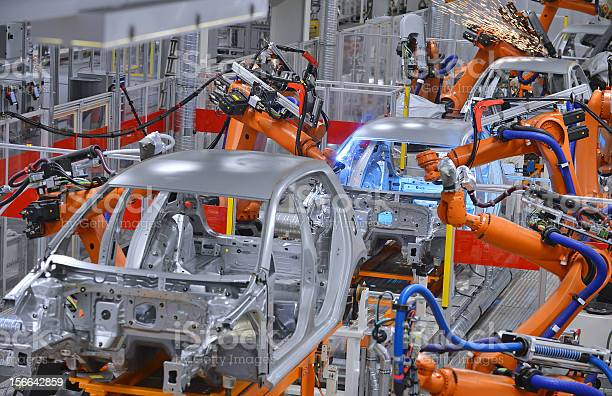
\includegraphics[width=8cm, keepaspectratio]{img/brazo}
    \caption{Brazo robótico.}
    \label{figura:brazo_robotico}
\end{figure}

En la actualidad cada vez son más populares los coches autónomos. Es un campo muy amplio que cuenta con un gran número de posibilidades. Alguna de estas posibilidades serían los coches con conducción autónoma de \textit{Tesla}  (Figura 1.2) o los coches con aparcamiento autónomo que están desarrollando un gran número de compañías en la actualidad, aspiradoras autónomas, inspección con drones, etc.

\begin{figure}[H]
	\centering
    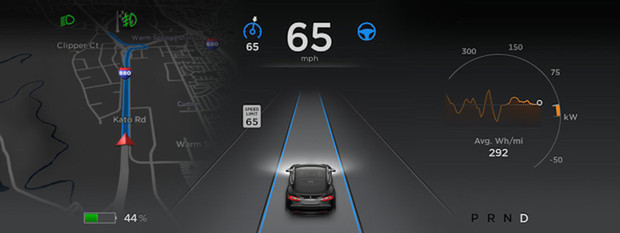
\includegraphics[width=8cm, keepaspectratio]{img/coche}
    \caption{Coche autónomo.}
    \label{figura:coche_autonomo}
\end{figure}

Otro campo de la aplicación de la robótica es la medicina, donde existen robots capaces de filtrar las vibraciones naturales del humano para proporcionarle una gran precisión y seguridad, un claro ejemplo es el robot DaVinci (Figura 1.3). Adicionalmente, hay robots capaces de mantener una estabilidad la estabilidad necesaria para caminar sobre dos piernas robóticas, como es el robot ATRIAS (Figura 1.4).

\begin{figure}[H]
  \centering
  \begin{minipage}[b]{0.4\textwidth}
    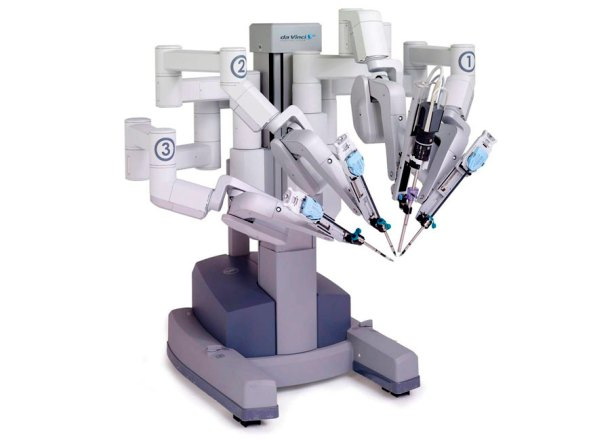
\includegraphics[width=\textwidth]{img/davinci}
    \caption{Robot DaVinci.}
    \label{figura:robot_davinci}
  \end{minipage}
  \hfill
  \begin{minipage}[b]{0.4\textwidth}
    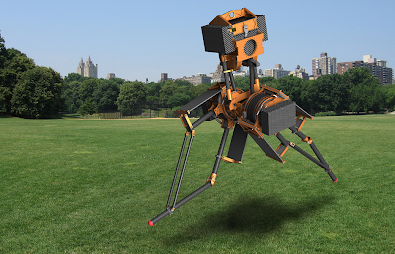
\includegraphics[width=\textwidth]{img/atrias}
    \caption{Robot ATRIAS.}
    \label{figura:robot_atrias}
  \end{minipage}
\end{figure}

En el ámbito militar, existen robots capaces de sustituir a una persona a la hora de realizar tareas de gran peligro como la desactivación de bombas y la entrada en zonas contaminadas (Figura 1.5).

\begin{figure}[H]
	\centering
    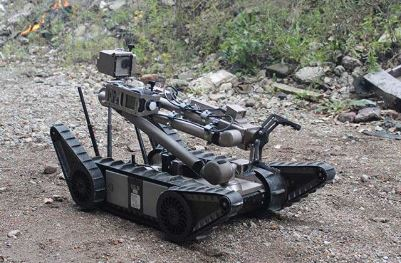
\includegraphics[width=8cm]{img/robot_militar}
    \caption{Robot militar.}
    \label{figura:coche_autonomo}
\end{figure}

\section{Componentes robóticas}
\label{subsec:componentes roboticas}

Todo robot está formado por dos componentes: el \textit{software}, encargado de proporcionar la inteligencia al robot, el más importante, y, el \textit{hardware} encargado de proporcionar la estructura física del robot.

Con al gran auge de la robótica han surgido numerosas plataformas que proporcionan herramientas que simplifican el desarrollo de software robótico, esto son los denominados \textit{middlewares} robóticos.

Durante el desarrollo de software robótico es preciso realizar una serie de pruebas para comprobar el funcionamiento del código y depurar errores, por lo que se necesitan simuladores que nos proporcionen un entorno cercano a la realidad previa al ensamblado del robot.

\subsection{Middlewares robóticos}
\label{subsec:middlewares}

Un \textit{middleware} robótico es un \textit{framework} que proporciona una serie de herramientas que facilitan el desarrollo de software para robots. Proporciona los servicios necesarios para soportar y simplificar aplicaciones complejas y distribuidas. Para el control de los sensores y actuadores de los robots, los \textit{middlewares} proporcionan \textit{drivers}, APIs, bibiliotecas con funcionalidad ya resuelta y reutilizables, etc.

\emph{OpenRDK} es un proyecto de código abierto para el desarrollo de módulos poco acoplados. Proporciona una gestión de concurrencia, comunicación entre procesos y una técnica de enlace que permite el diseño de sistemas conceptuales de puertos de datos de entrada / salida. También proporciona módulos para realizar conexiones con simuladores robóticos y controladores de robots genéricos. También existen algunos otros \emph{middlewares} como \emph{Micro} y \emph{Orca}.

El \textit{middleware} robótico más generalizado es ROS\footnote{\url{https://www.ros.org/}}
 (\textit{Robotics Operating System}). \textit{Robotics Operating System} fue desarrollado en 2007 por el Laboratorio de Inteligencia Artificial de Stanford para dar soporte a sus proyectos. A pesar de no ser un sistema operativo, ROS proporciona servicios como la abstracción \textit{hardware}, mecanismos de comunicación entre prosesos, el control de dispositivos de bajo nivel y el mantenimiento de paquetes. \textit{Robotics Operating System} fue desarrollado para sistemas UNIX, aunque en la actualidad está siendo adaptado para su funcionamiento en sistemas operativos como Fedora, Mac OS X, Arch, Gentoo, OpenSUSE, Slackware, Debian o Microsoft Windows.
 
Para transmitir información, ROS emplea un sistema de comunicación unidireccional llamado ROS \emph{Topics} \footnote{\url{http://wiki.ros.org/Topics}} (temas). Estos \emph{Topics} se comportan como buses sobre los cuales los nodos intercambian mensajes, además, son de publicación anónima.

Los \emph{Topics} tienen como objetivo una comunicación unidireccional de transmisión. Los nodos que necesitan hacer llamadas de procedimiento remoto que esperan una respuesta, deben emplear un servicio dedicado a ello.

Los ROS \emph{Nodes} \footnote{\url{http://wiki.ros.org/Nodes}} (nodos) son procesos que realizan cálculos. Los nodos se comunican entre sí mediante el uso de temas, servicios RPC (Remote Procedure Call) y un servidor de parámetros. Un sistema de control de un robot, generalmente está compuesto de un gran número de nodos, por ejemplo, un nodo controla un sensor láser, mientras que otro nodo controla los motores de las ruedas del robot.

Este \emph{middleware} ofrece una serie de herramientas \footnote{\url{http://wiki.ros.org/Tools}} para facilitarnos la visualización de la información que genera la aplicación robótica. Algunas de estas herramientas son las siguientes:
\nolinebreak
\begin{itemize}
\itemsep 0em
\item \textbf{RVIZ}: es un entorno de visualización 3D que permite combinar información de sensores, modelo del robot y otros datos en 3D en una vista combinada.
\item \textbf{Rqt-plot}: herramienta que permite visualizar datos escalares que generan los temas de ROS.
\item \textbf{Webviz}: una herramienta basada en navegador para buscar datos y archivos de ROS bags \footnote{\url{http://wiki.ros.org/Bags}}, incluso mezclados con vídeo en directo.
\end{itemize}

Además, también ofrece un amplio conjunto de \emph{drivers} que facilitan la incorporación de dispositivos adicionales en los robots, como cámaras, motores, láseres, sensores de posición, etc. Algunos de estos son:

\begin{itemize}
\itemsep 0em
\item \textbf{Cámara} \footnote{\url{http://wiki.ros.org/cv_camera}}: captura la imagen de la cámara y la publica en un tema llamado "\emph{sensor\_msgs\\/Image}"
\item \textbf{Motores} \footnote{\url{http://wiki.ros.org/Motor\%20Controller\%20Drivers}}: se encarga de publicar información relativa a los motores del robot, es decir, mensajes sobre la odometría y la posición del robot en distintos temas con la información de velocidad que recibe del tema "\emph{sensor\_msgs\\/Twist}"

\end{itemize}

\subsection{Simuladores robóticos}
\label{subsec:simuladores}

Los simuladores robóticos surgen con la necesidad de realizar pruebas durante el desarrollo del \textit{software} para la detección y depuración de posibles errores antes de llevarlo a un robot real debido al gran coste que suponen. En la actualidad, existen numerosos simuladores robóticos.

Uno de los simuladores más utilizados en la actualidad es \textit{Gazebo}\footnote{\url{http://gazebosim.org/}}. Su popularidad se debe a su robusto motor de físicas, sus gráficos de alta calidad y su amplio catálogo de robots y escenarios. Es una herramienta de código abierto integrada con ROS, por lo que permite ejecutar \textit{software} robótico en un escenario simulado (Figura 1.6).

\begin{figure}[H]
	\centering
    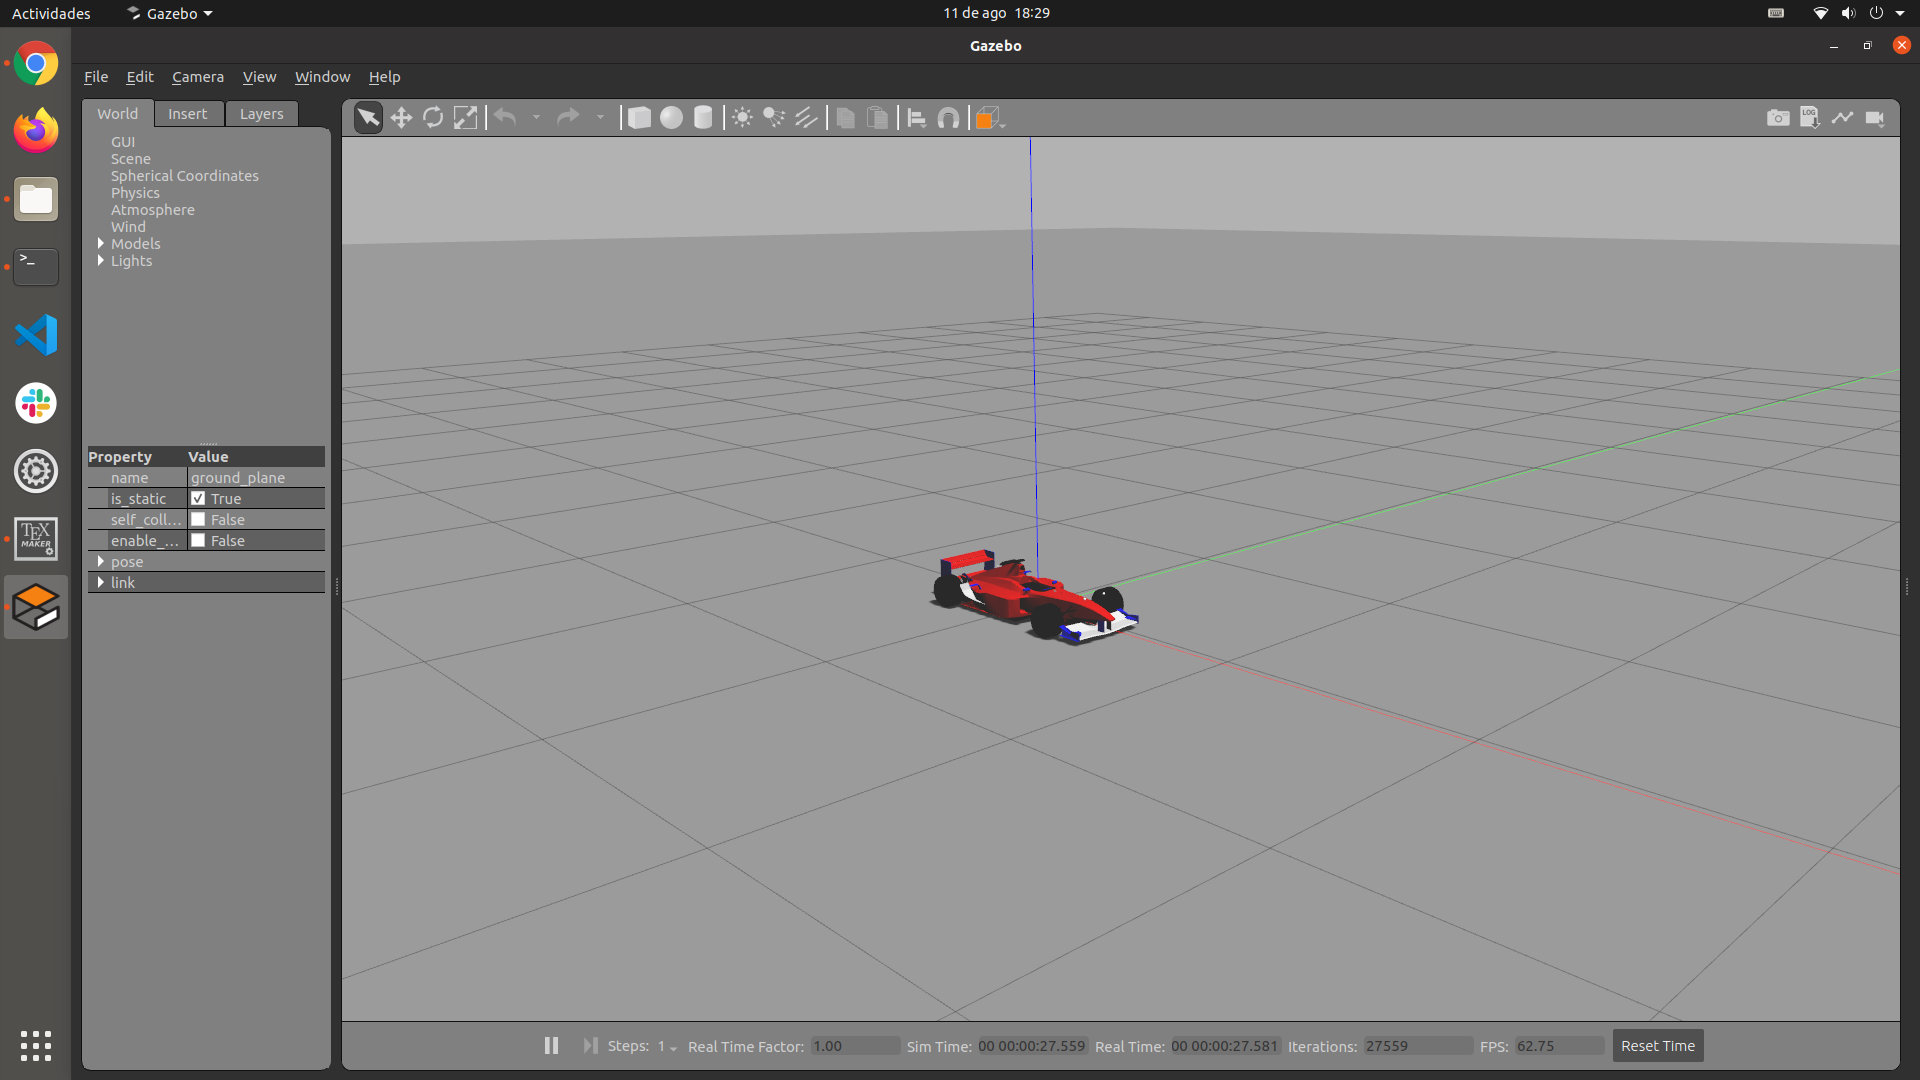
\includegraphics[width=\textwidth]{img/gazebo}
    \caption{Simulador Gazebo.}
    \label{figura:simulador_gazebo}
\end{figure}

\emph{CoppeliaSim} \footnote{\url{https://coppeliarobotics.com/}}. Se trata de un simulador robótico con un entorno de desarrollo integrado. se basa en una arquitectura de control distribuido: cada objeto/modelo se puede controlar individualmente a través de un script integrado, un complemento, un nodo ROS, un cliente API remoto o una solución personalizada. Los controladores pueden escribirse en  C/C++, Python, Java, Lua, Matlab u Octave.

\emph{Waymo} \footnote{\url{https://es.wikipedia.org/wiki/Waymo}} (Poryecto de vehículo autónomo de Google). Es una tecnología que permite a un vehículo moverse de forma autónoma por una ciudad y por carretera, detectando señales de tráfico, vehículos y demás objetos de la vía.

\emph{Carla} \footnote{\url{https://carla.org/}}. Es un sistema que se ha desarrollado desde cero para apoyar el desarrollo, entrenamiento y la validación de sistemas de conducción autónomos. \emph{Carla} provee su código, protocolos, sets de configuraciones de escenarios (zona urbana, edificios, veículos, etc) como fuente abierta. La plataforma admite un gran número de sensores, condiciones ambientales, un control completo de los actuadores, generación de terreno y mucho más.

\section{Robótica educativa}
\label{sec:robotica educativa}

La robótica educativa proporciona a los estudiantes la infraestructura para la construcción y programación de un robot, pero, además de la enseñanza robótica,
estos entornos van más allá, ofrenciendo la capacidad para el alumno de adquirir un pensamiento lógico. También, contribuye en la adquisición de una mentalidad resolutiva y al enriquecimiento de la cultura científica de los alumnos. Este método de educación con la robótica como objeto de enseñanza se denomina el método STEAM (Science, Technology, Engineering, Arts and Matemathics).

Como se ha comentado, para llevar a cabo este método de educación es necesaria una infraestructura, como alguna plataforma cuyo objetivo sea el de la enseñanza de la robótica, algunas de estas plataformas son las siguientes:

\begin{itemize}
\item \textbf{Robocode}: es un juego de programación en \emph{Java} o \emph{.NET}, cuyo objetivo es programar la lógica de un robot que es un tanque de batalla, para combatir contra otros tanques. Esta plataforma ofrece una comunidad que incluye uuna Wiki y un grupo de google. Además, ha realizado una competición propia \footnote{\url{https://gamesfleadh.ie/robocode/}}.
\item \textbf{OpenRoberta}: es un proyecto alemán que busca animar a los niños a programar mediante el uso de robots como \emph{Lego Mindstorms} y otros sistemas \emph{hardware} programables como \emph{Arduino}. Ofrece una plataforma en la nube llamada Open Roberta Lab, cuyo objetivo es simplificar los conceptos de programación la enseñanza de la programación en las escuelas. Es una plataforma gratuita y no requiere de instalaciones adicionales.
\item \textbf{CodeCombat}: ofrece un aprendizaje basado en juegos, tiene el objetivo de que los estudiantes aprendan mientras juegan. Los estudiantes aprenderán \emph{JavaScript}, \emph{Python}, \emph{HTML} y \emph{CoffeeScript}, además de aprender los fundamentos de la informática. El contenido se divide en 11 unidades: tres unidades de desarrollo de juegos, dos unidades de desarrollo web y seis unidades de informática.
\item \textbf{Gearsbot}: un entorno de programación de robots mediante bloques, que además también ofrece la posibilidad de programar la lógica en \emph{Python}, usa un simulador web que emplea la tecnología \emph{WebGL} \footnote{\url{https://es.wikipedia.org/wiki/WebGL}} para renderizar gráficos.
\item \textbf{Riders.ai}: una plataforma de programación de robots que ofrece la posibilidad de realizar competiciones idividuales como en grupos. Es accesible desde cualquier lado del mundo. También ofrece al usuario una capa de abstracción sobre los sensores, localización y diferentes partes del robot. En su plataforma online, proporciona una serie de cursos de iniciación a la robótica, además, ofrece un sistema de ligas en las que han de resolverse una serie de ejercicios, como forma de competición entre los usuarios. Esta plataforma está orientada a las competiciones, para empezar a aprender, el usuario ha de unirse a una competición y empezar a resolver los problemas de las misma, finalmente, obtendrá una puntuación en un ranking.
\item \textbf{TheConstruct}: ofrece un entorno de programación de robots que pueden moverse por la Luna, Marte y más planetas. No requiere la instalación de ROS. Ofrece un gran extra que le diferencia de los demás, esto es, brinda la posibilidad al usuario de poder ejecutar su código en robots reales de forma remota, y, también proveen certificados al completar diferentes cursos. La plataforma ofrece numerosos cursos de ROS, creación de robots, algoritmos robóticos, etc. Está orientada al aprendizaje mediante la práctica y no requiere ninguna instalación adicional. También ofrece una comunidad con la que los usuarios pueden interactuar.
\end{itemize}

Dentro de la robótica educativa, es preciso enfatizar la plataforma \textit{Unibotics} en la que se desarrolla el presente proyecto. Esta plataforma es un proyecto internacional que ofrece material para la enseñanza de robótica en las aulas. \textit{Unibotics} proporciona una infraestructura software en conjunto a una colección de ejercicios, cada uno con el material teórico correspondiente para su resolución. No requiere de ninguna instalación adicional. También ofrece una foro por el cual los usuarios pueden preguntar dudas, mostrar sus resultados y notificar acerca de bugs. De esta manera, se ofrece la posibilidad de aprender robótica con la necesiad de únicamente una conexión a internet.

\begin{figure}[H]
  \centering
  \begin{minipage}[b]{0.45\textwidth}
    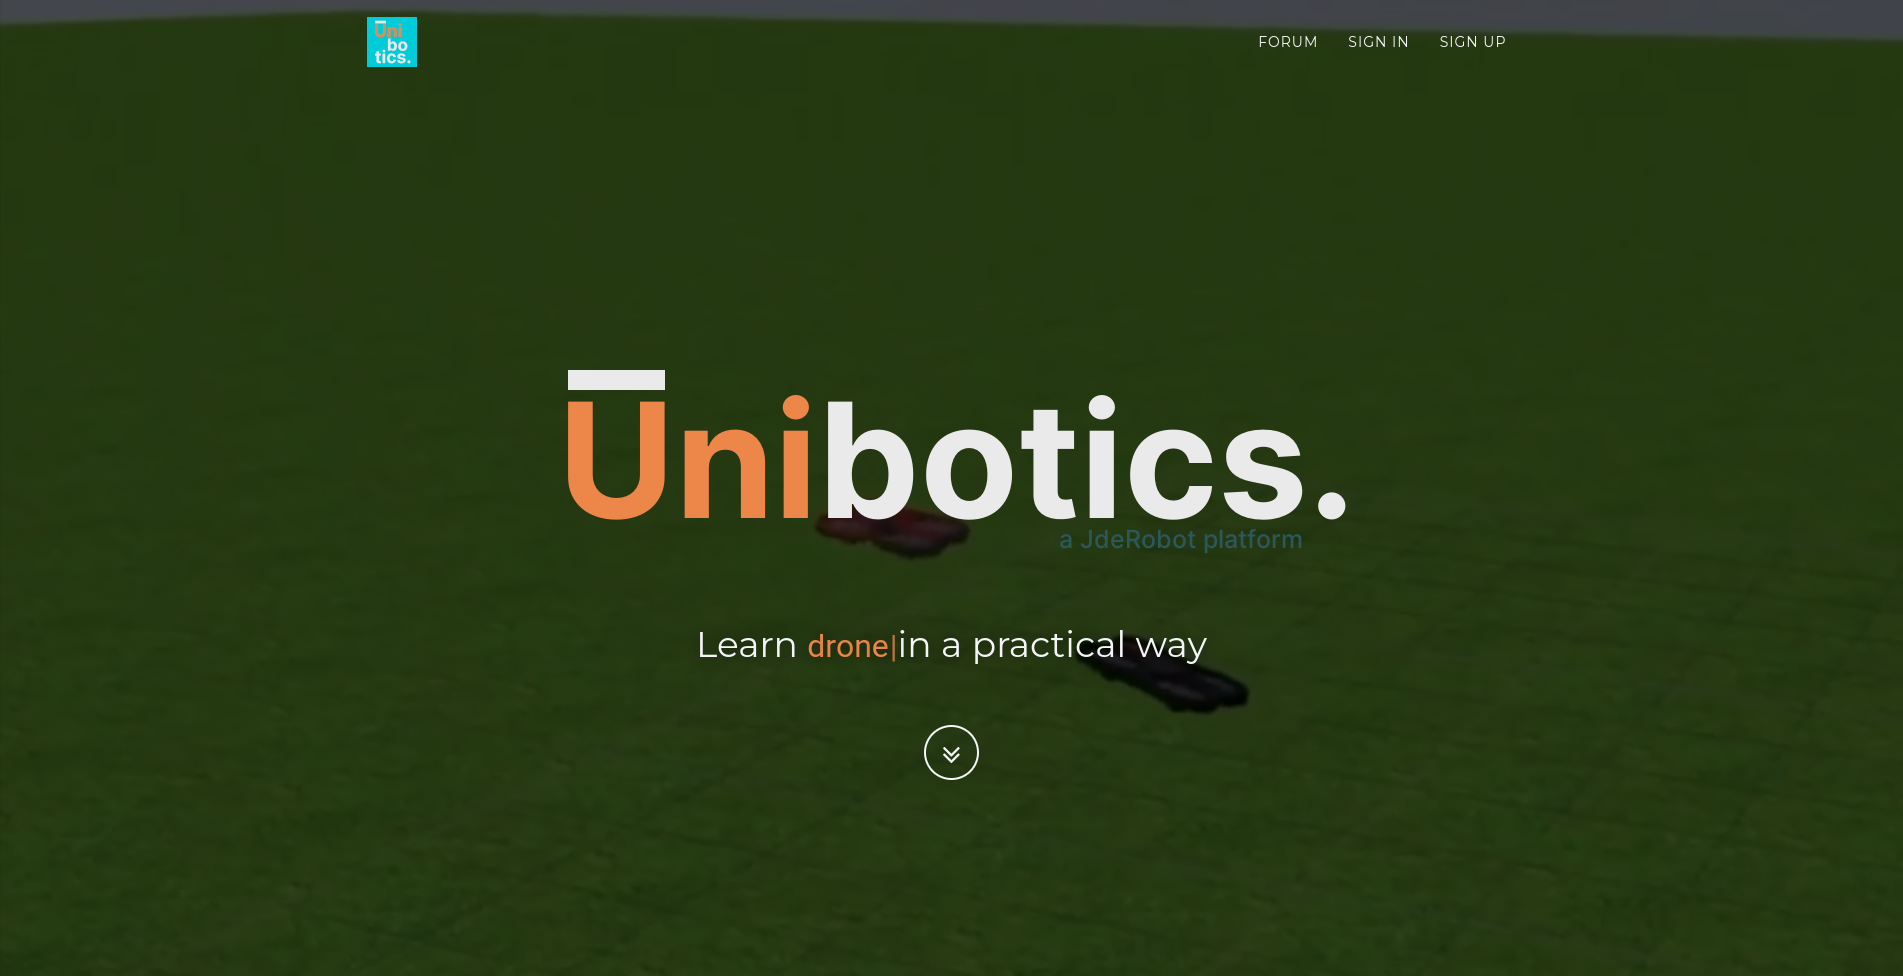
\includegraphics[width=\textwidth,height=45mm]{img/plataforma_unibotics.png}
    \caption{Plataforma de Unibotics.}
    \label{figura:stun}
  \end{minipage}
  \hfill
  \begin{minipage}[b]{0.45\textwidth}
    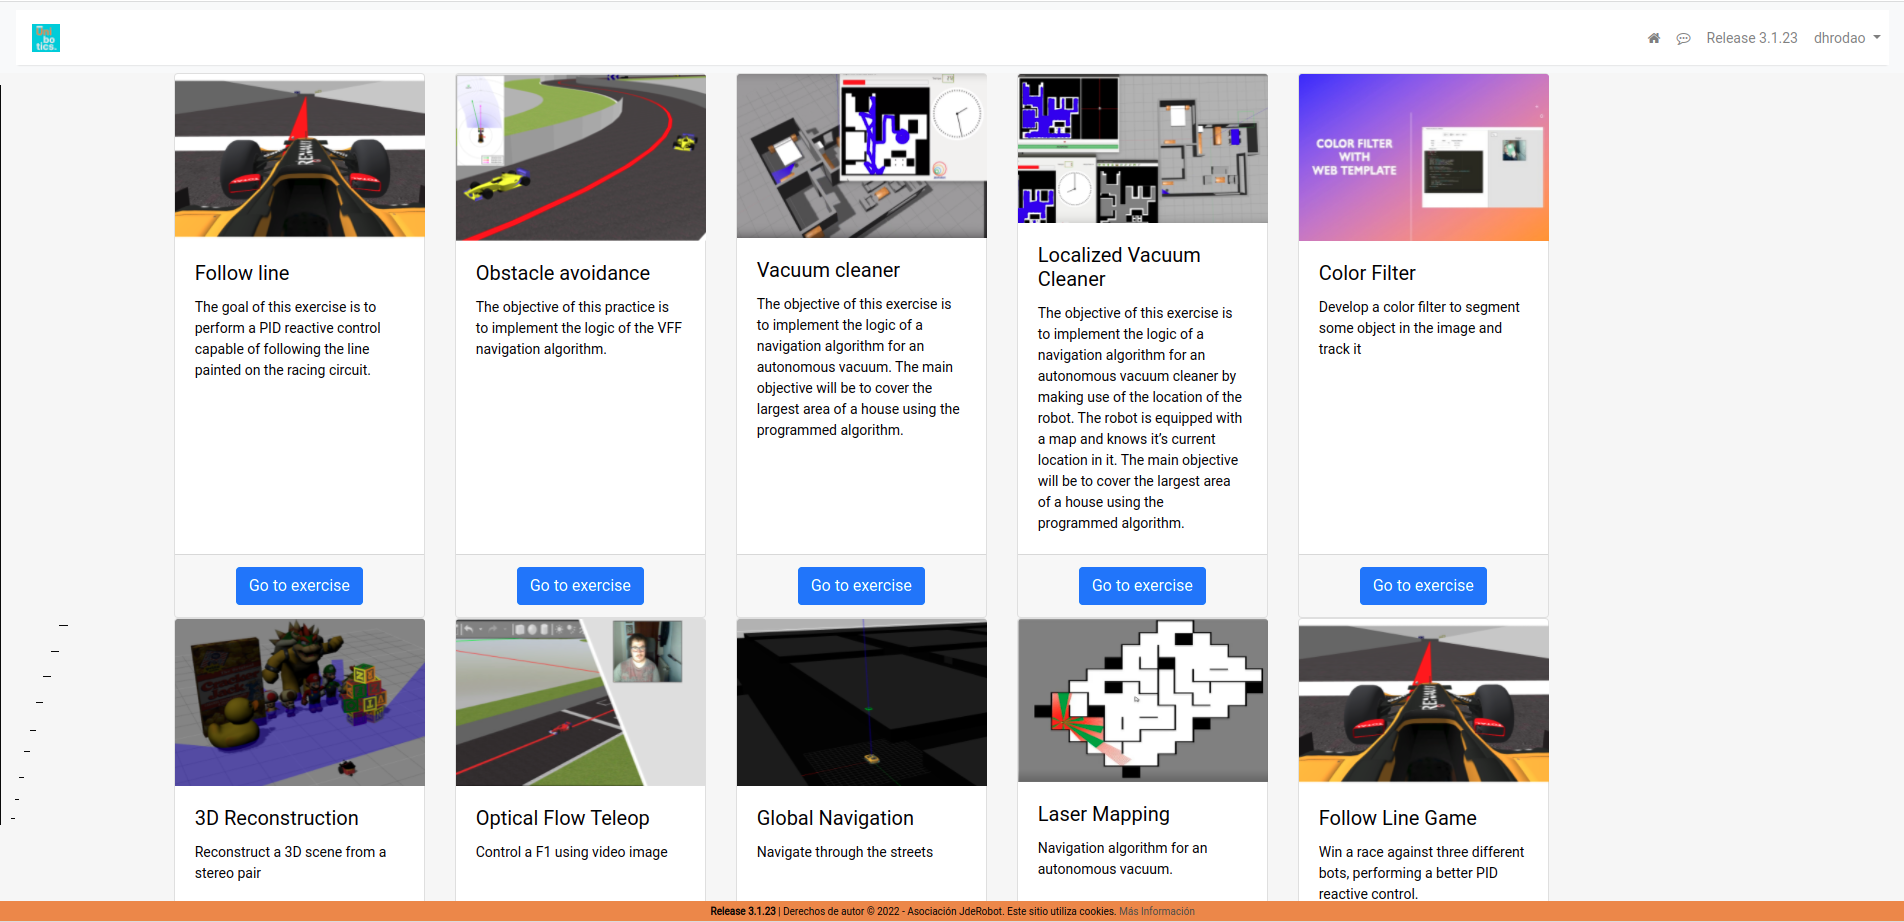
\includegraphics[width=\textwidth,height=45mm]{img/pagina_principal_unibotics.png}
    \caption{Página pricipal de Unibotics.}
    \label{figura:turn}
  \end{minipage}
\end{figure}

Esta plataforma permite el aprendizaje de la robótica mediante una serie de ejercicios que se muestran a través de una interfaz web. Ofrece un amplio rango de ejercicios con robots de todo tipo, como coches, drones y aspiradoras, con distintos tipos de sensores como sensores de proximidad láser, cámaras, diversos motores y sensores de navegación.

La gamificación de la educación tiene una gran importancia, pues potencia las capacidades de los estudiantes, además, aumenta la concentración y la motivación. De manera que hace que los estudiantes puedan alcanzar un nivel de conocimiento superior con la unión de actividades lúdicas y aprendizaje.


\section{Tecnologías Web}

Las diferentes tecnologías web permiten crear interfaces de usuario y establecer las comunicaciones con el servidor, además de implementar comportamientos de la web en el servidor. Se pueden distinguir en tecnologías \emph{backend} (del lado del servidor) y tecnologías \emph{frontend} (del lado del usuario).

Una gran ventaja de estas tecnologías es que ofrecen la ausencia de la necesidad de instalar componentes de software, configuración y dependencias adicionales. Únicamente es necesario disponer de un navegador de internet y una conexión a internet, pues todos los archivos necesarios se servirán desde el lado del servidor. Además, tambien permiten una compatibilidad multiusuario, es decir, no es necesaria la instalación de software adicional ni de ningún sistema operativo en específico, pues es únicamente necesario un navegador web y una conexión a internet para el uso de una aplicación web.

En la actualidad existen numerosas aplicaciones web de las que hacemos uso en el día a día, estas pueden ser, aplicaciones bancarias, la tienda de \emph{Amazon}, aplicaciones de videoconferencia como \emph{Google Hangouts}, tiendas online de productos de comida (\emph{Uber Eats}), e incluso aplicaciones de venta de productos de segunda mano (\emph{Wallapop}). A día de hoy un gran número de empresas proveen a sus usuarios de estas aplicaciones web, pues ofrecen una compatibilidad universal, y, además, del lado del usuario, este no tiene que instalar ninguna aplicación. 

Estas tecnologías facilitan el uso al cliente, pues evitan que el usuario tenga que intalar actualizaciones, pues las actualizaciones se realizan en el lado del servidor. Esta ventaja elimina posibles fallos debidos a incompatibilidades entre las versiones, pues el servidor distribuye una única version para todos. También ofrecen la ventaja de aplicaciones web multiplataforma, únicamente es necesario el desarrollo en un único entorno (\emph{Windows}, \emph{Ubuntu}, \emph{MacOS}, etc), pues estas tecnologías son comunes a los navegadores de todos los sistemas. Únicamente es necesario conocer \emph{HTML}, \emph{CSS} y \emph{JavaScript}, el navegador será el encargado de interpretar dichos lenguajes.

Las aplicaciones web dependen de una conexión entre el usuario y el servidor, por lo que, una de las desventajas que estas es la latencia que esta conexión pueda generar. Estas tecnologías siempre son algo más lentas que otros lenguajes compilados como \emph{C\#} puesto que el navegador no realiza ninguna compilación, si no que interpreta el código línea a línea.

En el lado del servidor, existen diversos \emph{frameworks} que facilitan la vida al desarrollador. Algunos ejemplos de ellos serían, \emph{Express} para el lenguaje \emph{JavaScript} y \emph{Django} escrito en \emph{Python}.

El desarrollo de tecnologías web está sujeto a un gran crecimiento. Cada vez las aplicaciones web son más potentes y eficientes, de manera que cada vez son más los desarrolladores que optan por este modelo de desarrollo.

Las tecnologías web ofrecen la posibilidad de que varios usuarios puedan programar robots y ejecutarlos en el mismo escenario, hacer competiciones tanto síncronas como asíncronas, algo que resultaría muy complejo si se realizase en local. \emph{WebRTC} nos ofrece esta posibilidad, pues es una herramienta de código abierto que proporciona conexiones en tiempo real entre \emph{peers} mediante un API.

\section{Estructura del documento}

En esta sección se va a hacer un breve resúmen de los contenidos de cada capítulo, también se mencionará como están estructurados.

En el capítulo 2, Objetivos, se explica cuál es el propósito o los propósitos de este trabajo. También se mencionará la planificación temporal que se ha llevado a cabo durante el trabajo. Y finalmente, se mencionará la heramienta empleada para realizar un control de versiones.

Posteriormente, en el capítulo 3, Herramientas, se habla exclusivamente sobre las herramientas y tecnologías utilizadas. Serán descritas indicando sus ventajas, inconvenientes y áreas de uso.

A continuación, en el capítulo 4, Juegos Asíncronos, se explicará cómo se ha realizado el diseño de los mismos, tanto para la IU como para la infraestructura interna.

Seguidamente, en el capítulo 5, Juegos Síncronos, de igual manera que en la sección anterior, se explicará como se ha desarrollado la infraestructura necesaria para elaborar el ejercicio.

Finalmente, en el capítulo 6, tenemos los experimentos realizados y sus resultados, además, en el capítulo 7, se encuentran las conclusiones obtenidas de haber realizado este trabajo, y, en último lugar la bibliografía que contiene todos los contenidos empleados para el desarrollo del trabajo.

%%%%%%%%%%%%%%%%%%%%%%%%%%%%%%%%%%%%%%%%%%%%%%%%%%%%%%%%%%%%%%%%%%%%%%%%%%%%%%%%
%%%%%%%%%%%%%%%%%%%%%%%%%%%%%%%%%%%%%%%%%%%%%%%%%%%%%%%%%%%%%%%%%%%%%%%%%%%%%%%%
% OBJETIVOS %
%%%%%%%%%%%%%%%%%%%%%%%%%%%%%%%%%%%%%%%%%%%%%%%%%%%%%%%%%%%%%%%%%%%%%%%%%%%%%%%%

\cleardoublepage % empezamos en página impar
\chapter{Objetivos} % título del capítulo (se muestra)
\label{chap:objetivos} % identificador del capítulo (no se muestra, es para poder referenciarlo)

En este capítulo se explicarán los objetivos concretos que se pretenden alcanzar en este TFG, los requisitos para los problemas que se van a plantear, la planificación y metodología seguida durante todo el desarrollo.

\section{Objetivos} % título de sección (se muestra)
\label{sec:objetivo-general} % identificador de sección (no se muestra, es para poder referenciarla)

El objetivo general de este trabajo es la introducción de juegos en la plataforma \emph{Unibotics}, en los que varios usuarios puedan competir síncrona y asíncronamente para fomentar su aprendizaje. Este objetivo principal se ha dividido en dos subobjetivos.

\begin{itemize}
\item La introducción de \textbf{juegos competitivos asíncronos} que permitan a los usuarios competir contra una serie de oponentes automśticos proporcionadas por la plataforma, en el mismo escenario y en tiempo real.
\item La introducción de \textbf{juegos competitivos síncronos} que proporcionan una visión más competitiva y social de la plataforma a los usuarios, que pueden conectarse simultáneamente con sus amigos para competir entre ellos. Este juego se basará en tecnologías WebRTC.
\end{itemize}

Las soluciones proporcionadas deben cumplir los objetivos previamente mencionados, además de los siguientes requisitos para una correcta implementación:

\begin{itemize}
\item El código del frontend del servidor debe ser desarrollado en \emph{HTML}, \emph{CSS3} y \emph{JavaScript}.
\item El código del backend se desarrollará en Python utilizando Django.
\item No debe requerir instalaciones de software adicionales en el uso regular de \emph{Unibotics}, el usuario unicamente ha de tener el contenedor docker instalado en la máquina local.
\end{itemize}

\section{Metodología}
\label{sec:metodologia}

Para llevar a cabo este trabajo, se ha empleado una metodología basada en \emph{sprints} \footnote{\url{https://www.bbva.com/es/metodologia-scrum-que-es-un-sprint/}}. Este modelo de desarrollo se corresponde con un modelo de desarrollo de software ágil, consiste en dividir un proyecto en tareas más sencillas y de menor duración, de forma que cada cierto período de tiempo (1-2 semanas) puedan presentarse resultados. Esta metodología es muy útil pues, es susceptible a cambios por parte del cliente.

Para la implantación de esta metodología se han establecido reuniones semanales. En dichas reuniones se ha comentado los cambios que se han introducido en el \emph{sprint} previo para proponer cambios, mejoras y fijar una serie de objetivos para la siguiente semana.

El proyecto de \emph{Unibotics} es amplio y se apoya en varios repositorios software en GitHub. Con el fin de incorporar cambios en el código del proyecto relacionados con este TFG, se ha empleado la herramienta \emph{GitHub}. La metodología que se ha seguido para incorporar nuevos cambios a los diferentes repositorios es la siguiente. En primer lugar se crea una incidencia (\emph{issue}) en el repositorio correspondiente que describa el problema que se va a resolver. A continuación, se crea una rama a partir de la rama \emph{master} con el nombre de \emph{issue-XXX} donde se incorporarán todos los cambios mencionados en la incidencia que se creó. Finalmente, una vez se han realizado todos los cambios y se ha verificado que funciona de manera correcta, se realiza un parche (\emph{Pull Request}), esto es, una solicitud de incorporación de los cambios a la rama principal. Los parches son revisados por otro compañero, que se encargará de hacer la pruebas pertinentes e incorporarla a la rama \emph{master}.

En este proyecto se ha trabajado con los siguientes repositorios:

\begin{itemize}
\item \textbf{unibotics-webserver:} aquí se encuentran los recursos del webserver Django.
\item \textbf{unibotics-exercises:} este repositorio contiene las plantillas de los ejercicios de la plataforma.
\item \textbf{RoboticsAcademy:} este repositorio es una colección \emph{open-source} de algunos retos, que se han empleado para diseñar ejercicios para la plataforma de \emph{Unibotics}.
\item \textbf{CustomRobots:} este repositorio contiene todos los robots empleados en las simulaciones.
\item \textbf{noVNC:} se ha realizado un \emph{fork} del repositorio oficial puesto que para la versión del ejercició síncrono se necesitaba hacer algunas modificaciones para enviar el flujo de vídeo al extremo remoto.
\end{itemize}

\section{Plan de trabajo}
\label{sec:plan-de-trabajo}

Para el seguimiento de los objetivos previamente mencionados, se ha seguido una serie de etapas que permiten el avance incremental en la implementación del trabajo.

\begin{itemize}
\item \textbf{Estudio de la plataforma Unibotics:} Como una primera toma de contacto es preciso el estudio de la infraestructura técnica que se está empleando en la plataforma. Además, se ha realizado la puesta en funcionamiento del \emph{despliegue local} \footnote{Despliegue de un clon de la plataforma en un entorno local con el fin de realizar cambios y probar nuevas funcionalidades, previo a incorporar los cambios a la plataforma oficial}, el contenedor docker (\emph{RADI}) y la comprobación de que todos los ejercicios funcionan de manera correcta. También, se ha estudiado el funcionamiento de las plantillas empleadas por los ejercicios y la conexión con el \emph{RADI}.

\item \textbf{Desarrollo de los juegos asíncronos:} Una vez entendidos los conceptos principales de la plataforma, se ha procedido al desarrollo de los juegos asíncronos. Se han diseñado nuevas plantillas web para los nuevos ejercicios asícronos, y, añadido nuevos aspectos, como evaluadores automáticos.

\item \textbf{Estudio de la tecnología WebRTC:} Una vez completada la parte de los juegos asíncronos, se procede al estudio de estas tecnologías de videoconferencia que permiten la retransmision de audio y vídeo entre dos navegadores web. Se han desarrollado algunos pequeños programas de prueba, como un chat de texto y vídeo, para asentar los conceptos.

\item \textbf{Desarrollo del juego síncrono:} Con los conceptos de WebRTC asentados, se ha procedido a diseñar en el webserver de \emph{Unibotics}, un sistema de señalización entre los usuarios, de manera que se pueda intercambiar la información necesaria para realizar la conexión WebRTC. Finalmente, en las plantillas del ejercicio, se incluye código \emph{JavaScript} que se encarga de establecer las conexiones RTC para cada extremo.
\end{itemize}

%%%%%%%%%%%%%%%%%%%%%%%%%%%%%%%%%%%%%%%%%%%%%%%%%%%%%%%%%%%%%%%%%%%%%%%%%%%%%%%%
%%%%%%%%%%%%%%%%%%%%%%%%%%%%%%%%%%%%%%%%%%%%%%%%%%%%%%%%%%%%%%%%%%%%%%%%%%%%%%%%
% HERRAMIENTAS %
%%%%%%%%%%%%%%%%%%%%%%%%%%%%%%%%%%%%%%%%%%%%%%%%%%%%%%%%%%%%%%%%%%%%%%%%%%%%%%%%

\cleardoublepage % empezamos en página impar
\chapter{Herramientas} 
\label{chap:herramientas}

En este capítulo se hará una breve presentación de todas las herramientas empleadas para el desarrollo del presente TFG. Estas tecnologías se pueden englobar en cuatro grupos, las tecnologías Front-End dedicadas a la presentación y a la interfaz de usuario (JavaScript, HTML y CSS), tecnologías Back-End dedicadas al servidor (Django), tecnologías WebRTC que serán las utilizadas en la retransmisión del vídeo en los juegos síncronos, y, por último, tecnologías dedicadas al control de versiones (GitHub). 

Estas herramientas son estandarizadas por medio de W3C \footnote{\url{https://www.w3.org}} (World Wide Web Consortium). Además, la versión de HTML empleada para realizar este trabajo es \emph{HTML5}, pues es la versión establecida por W3C como lenguaje de hipertexto de la World Wide Web.

\section{Lenguaje JavaScript}
\label{sec:javascript}

Su estándar se denomina \textit{ECMAScript}\footnote{\url{https://es.wikipedia.org/wiki/ECMAScript}}. Se trata de un lenguaje de programación interpretado, basado en \textit{Java} y \textit{C}. Fue creado para aplicaciones web del lado del cliente. Es interpretado en el navegador web y permite mejoras en la interfaz de usuario, además de páginas web dinámicas. También puede usarse en el lado del servidor utilizando \textit{Node.js}, un entorno de ejecucción de JavaScript construido con el motor \textit{JavaScript V8}.

En este proyecto se ha empleado JavaScript en el lado de la interfaz de usuario. La lógica de las plantillas que usan los ejercicios ha sido programada usando \textit{ECMAScript-6}, es decir, se ha empleado para los controladores de los botones de la interfaz, para comunicaciones entre la interfaz de usuario con determinados sevicios, y, además, para todos los extras añadidos a los ejercicios base de los que se parten. Sus principales características son:

%\subsection{Caractrerísticas del lenguaje}
%\label{subsec:javascript}

\begin{itemize}
	\item Originalmente se trata de un lenguaje del lado del cliente, es decir, típicamente ejecuta en la máquina del propio cliente a través de un navegador.
	
	\item Tipado débil, por lo que no es necesario especificar el tipo de dato al declarar una variable permitiendo que una misma variable pueda adquirir distintos tipos durante la ejecucción.
	
	\item De alto nivel, con lo que significa que su sintaxis es fácilmente comprensible para las personas. Esta sintaxis se encuentra alejada del lenguaje máquina.
	
	\item Es un lenguaje interpretado puesto que utiliza un intérprete que traduce las líneas de código a lenguaje máquina en tiempo de ejecución.

	\item Es un lenguaje orientado a objetos, ya que utiliza clases y objetos como estructuras.
\end{itemize}

Adicionalmente, en este Trabajo de Fin de Grado, junto con \textit{ES-6} se ha empleado una librería llamada \textit{jQuery} que permite agregar dinamismo a un sitio web permitiendo interactuar con los elementos HTML, manipular el DOM, manejar eventos, diseñar animaciones y agregar interacción con la técnica \textit{AJAX}\footnote{\url{https://developer.mozilla.org/es/docs/Web/Guide/AJAX}} (\textit{Asynchronous JavaScript and XML}).

\subsection{Librería jQuery}
\label{subsec:javascript}

\textit{jQuery} \footnote{\url{https://jquery.com/}} es una librería multiplataforma desarrollada en JavaScript, inicalmente desarrollada por John Resig. Esta librería permite simplificar en gran medida la interacción con los documentos HTML y sus estilos, manipular el DOM, manejar eventos, crear animaciones, y agregar la integración de la técnica \textit{AJAX} (\textit{Asynchronous JavaScript and XML}). La versión utilizada en este proyecto es \emph{jQuery 3.3.1}.

Gracias a esta librería, es posible diseñar una interfaz gráfica elaborada sin necesidad de tener amplios conocimientos de CSS.
\section{Lenguaje HTML}

\textit{HTML} \footnote{\url{https://developer.mozilla.org/es/docs/Web/HTML}} (\textit{HyperText Markup Languaje}) es un lenguaje de marcado que permite indicar la estructura un documento utilizando etiquetas. Es utilizado para la creación de documentos electrónicos que se envían a través de la red. Los documentos pueden tener conexiones con otros a través de \textit{hipervínculos}.

\begin{figure}[H]
	\centering
    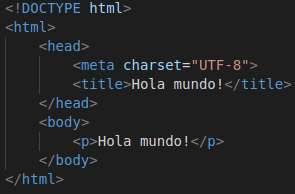
\includegraphics[width=8cm]{img/html}
    \caption{Documento básico de \textit{HTML}.}
    \label{figura:simulador_gazebo}
\end{figure}

Primeramente se debe declarar el tipo del documento \textit{HTML} mediante la línea \textit{DOCTYPE html} que indica que es un documento \textit{HTML-5}. El elemento \textit{html} engloba el documento \textit{HTML}, dentro de este elemento se encuentran dos etiquetas:

\begin{itemize}
	\item \textit{HEAD} es la cabecera del documento, que contiene la información general (metadatos) acerca del documento, incluyendo el título y los enlaces a scritps y hojas de estilos.
	
	\item \textit{BODY} es el cuerpo del documento \textit{HTML} donde se encuentran las etiquetas que dan formato al mismo. Puede contener imágenes, enlaces, vídeos, menús, formularios, botones, además de animaciones, que se pueden crear dentro de un elemento canvas.
\end{itemize}

Con la incorporación de \textit{HTML-5} se han introducido diversas novedades y mejoras que son de interés para este trabajo:

\begin{itemize}
\itemsep 0em
\item \textit{WebSockets} \footnote{\url{https://developer.mozilla.org/es/docs/Web/API/WebSockets_API}}, es una tecnología que hace posible abrir una comunicación de baja latencia entre el navegador y el servidor.
\item \textit{WebRTC} \footnote{\url{https://webrtc.org/}} (\textit{Web Real-Time Communications}) es una tecnología que permite a las aplicaciones web capturar y transmitir audio y vídeo entre navegadores sin necesidad de un intermediario.
\item Se añade un mejor soporte de contenido multimedia sin la necesidad de instalar plugins adicionales. Mediante el elemento \textit{video} en la página web del navegador reproducirá de manera nativa el contenido audiovisual.
\item Proporciona un elemento, \textit{canvas} que permite renderizar escenas gráficas en la web mediante el uso de \textit{JavaScript}.
\end{itemize}

\section{Hojas de estilo CSS}
\label{sec:css}

CSS \footnote{\url{https://developer.mozilla.org/es/docs/Web/CSS}} o \textit{Cascading StyleSheet} es un lenguaje empleado para dar formato y estilo a un documento de texto, comunmente, las instrucciones se agrupan en archivos con extensión \textbf{*.css}. Lo que permite que para una página web se puedan almacenar estilos por separado dependiendo del fin de cada uno. Además, la posibilidad de agrupar las instrucciones en varios archivos hace posible la importación en cada documento únicamente las instrucciones de las que se va a hacer uso.

Al poder almacenar las instrucciones ficheros separados, esto ofrece una gran ventaja, es decir, la separación de la estructura del documento (HTML) de su representación (CSS). También es posible añadir instrucciones CSS en la cabecera de un documento HTML mediante la etiqueta \textit{style}, pero  no se considera una buena práctica.

A continuación se muestra un ejemplo del uso de este lenguaje.

\begin{figure}[H]
	\centering
    
\includegraphics[width=15cm]{img/nocss_vs_css}
    \caption{Comparativa entre no usar CSS (izquierda) y usarlo (derecha).}
    \label{figura:nocss_vs_css}
\end{figure}

Como se puede apreciar en la imagen 3.2, hay un gran salto de no usar CSS a usarlo en los documentos HTML. Este lenguaje permite diseñar barras de navegación, menús desplegables, barras de búsqueda, botones, sub-apartados, etcétera, personalizados al estilo que se le quiera dar a la página, y con una apariencia muy diferente a los elementos que ofrece HTML por defecto.

CSS también permite la creación de páginas web responsivas, esto es, que los elementos se coloquen de una manera u otra para ofrecer una mejor disposición de los elementos dependiendo del tamaño la pantalla del usuario. Es decir, un teléfono móvil no tiene una pantalla de las mismas dimensiones que un ordenador, por lo que en el caso de una pantalla de un teléfono, con una web responsiva los elementos se colocarían de determinada manera para que sea más cómoda la experiencia del usuario, y, por ejemplo, que el usuario no tenga que hacer desplazamientos horizontales para ver el contenido, o que los botones y la fuente se adapten tomando un mayor tamaño de manera que sean legibles.

\section{Django para servidores web}
\label{sec:django}

Django \footnote{\url{https://es.wikipedia.org/wiki/Django_(framework)}} \cite{django} es un entorno de alto nivel basado en el lenguaje Python que facilita el desarrollo de sitios web seguros y sostenibles, en este proyecto en particular, se ha empleado \emph{Django 2.2}. Fue lanzado como un \emph{framework} web genérico en 2005, bajo una licencia de código abierto. Django se encarga de las complicaciones del desarrollo web (como puede ser la seguridad, la autenticación de usuarios, expresiones regulares predefinidas para validaciones de campos como correos´), para que el usuario pueda centrarse en escribir su aplicación.

El objetivo de Django es la creación sencilla de sitios web complejos, poniendo énfasis en la reutilización, la conectividad y la extensibilidad de componentes, el desarrollo rápido y el principio de no repetir código (\textit{Don't Repeat Yourself}).

Algunas de las carácterística de Django son:

\begin{itemize}
\item Un mapeador objeto-relacional, es capaz de convertir datos entre un sistema de tipos utilizado en un lenguaje de programación orientado a objetos y la utilización de una base de datos relacional. Permite realizar accesos a las bases de datos utilizando los filtros del lenguaje Python, no es necesario utilizar el lenguaje SQL de consultas a bases de datos. Django traduce automáticamente de Python a peticiones SQL.

\item Aplicaciones incorporables en cualquier página gestionada con Django.

\item Una API de base de datos robusta y genérica. Soporta MySQL, SQLite, Postgre, y demás sistemas de bases de datos y a las que el programador del sitio web accede con el uso de Python.

\item Un sistema incorporado de "vistas genéricas" que ahorra el tener que escribir la lógica de ciertas tareras comunes.

\item Un sistema extensible de plantillas con herencia, que simplifican la programación de páginas web dinámicas, que se autocompletan en tiempo de ejecución
dependiendo de las consultas del usuario.

\item Un despachador de URLs basado en expresiones regulares.

\item Un sistema \textit{middleware} para desarrollar caracteríscas adicionales.

\item Soporte de internacionalización, incluyendo traducciones de la interfaz de administración.

\item Documentación incorporada accesible a través de la aplicación administrativa.
\end{itemize}

\section{WebRTC}
\label{sec:webrtc}

WebRTC \footnote{\url{https://es.wikipedia.org/wiki/WebRTC}} \cite{webrtc} (Web Real-Time Communication) es un proyecto libre y de código abierto que proporciona una comunicación en tiempo real (RTC) a través de una serie de APIs. Permite que la transmisión de audio y vídeo funcione dentro de las páginas web al permitir la comunicación \textit{Peer to Peer}, sin necesidad de instalación de plugins y sin necesidad de la intervención del servidor. WebRTC tiene soporte en los navegadores Safari, Chrome, Firefox, Mozilla y Opera, está estandarizado por el World Wide Web Consortium \footnote{\url{https://es.wikipedia.org/wiki/World_Wide_Web_Consortium}} y por el Internet Engineering Task Force \footnote{\url{https://es.wikipedia.org/wiki/Grupo_de_Trabajo_de_Ingenier\%C3\%ADa_de_Internet}}.

El API de WebRTC tiene una serie de interfaces principales que son clave en el desarrollo del software para este proyecto:

\begin{itemize}
\item \textbf{RTCPeerConnection} \footnote{\url{https://developer.mozilla.org/es/docs/Web/API/RTCPeerConnection}} representa una conexión entre una máquina local y un par remoto. Esta interfaz provee métodos para: conectar un equipo remoto, mantener y monitorizar esa conexión y cerrar la conexión.

\item \textbf{RTCDataChannel} \footnote{\url{https://developer.mozilla.org/en-US/docs/Web/API/RTCDataChannel}} representa el canal que puede ser empleado para la transmisión de datos de baja lantencia (pues está basado en el protocolo UDP) entre pares (\textit{Peer to Peer}).

\item \textbf{MediaDevices} \footnote{\url{https://developer.mozilla.org/es/docs/Web/API/MediaDevices}} proporciona el acceso desde el navegador web a los dispositivos multimedia conectados, como webcams y micrófonos, y, también para compartir la pantalla. Ofrece un método \textit{getUserMedia()}, que, con el permiso del usuario, enciende la cámara, obtiene la imagen de la pantalla, el audio del micrófono, y, proporciona un \textit{MediaStream} que contiene pistas de vídeo y/o de audio del dispositivo.

\item \textbf{MediaStream} \footnote{\url{https://developer.mozilla.org/en-US/docs/Web/API/MediaStream}} representa el flujo de contenido multimedia. Un flujo consiste de varias pistas, ya sean de audio o de vídeo.
\end{itemize}

\subsection{Protocolos y mecanismos de comunicación}
\label{subsec:protocolos}

\begin{itemize}
\item \textbf{ICE} \footnote{\url{https://en.wikipedia.org/wiki/Interactive_Connectivity_Establishment}} (\textit{Interactive Connectivity Establishment}). Es una técnica empleada para permitir que un navegador web se conecte con otro/s navegador/es web mediante conexiones entre pares. Debe poder pasar por un \textit{firewall}, dirección IP pública, y, transmitir los datos a través de otro servidor, si el \textit{router} no permite las conexiones directas entre pares. Para lograr esta serie de casos, se emplean servidores STUN y TURN. Previo al establecimiento de una conexión ICE, es necesario realizar una señalización, que sirve para que ambos pares negocien un tipo de conexión. Para poder realizar una negociación satisfactoria, es necesario un servidor intermedio (servidor de señalización) que se encarge de comunicar ambos extremos durante el proceso de señalización.

\item \textbf{NAT} \footnote{\url{https://en.wikipedia.org/wiki/Nat}} (\textit{Network Address Translation}). Es empleado por el \textit{router} para asignar una dirección IP pública. El \textit{router} tiene acceso a la dirección pública de cada dispositivo y cada dispositivo conectado a este, tendrá una dirección IP privada. Las solucitudes se traducen de la IP privada a la IP pública con un puerto único. Desde el exterior de una red privada todos los dispositivos tienen la misma IP pública, de manera que el router se encarga de entregar el mensaje al dispositivo que corresponda, esto permite ahorrar direcciones IP, pero complica la comunicación directa entre dispositivos que se encuentren detras de sus respectivos NATs. Algunos \textit{enrutadores} tienen restricciones sobre quién puede conectarse a su red. Esto puede dar lugar a que aunque tengamos un única dirección IP pública encontrada por el servidor STUN, no se pueda establecer una conexión. Ante este caso, se debe recurrir a un servidor TURN.

\item \textbf{STUN} \footnote{\url{https://en.wikipedia.org/wiki/STUN}} (\textit{Session Transversal Utilities for NAT}). Es un protocolo de descubrimiento de IP pública, para determinar cualquier restricción en el \textit{enrutador} que impida una conexión directa con un par. El cliente enviará una solicitud STUN en Internet que responderá con la dirección pública del cliente y si el cliente esta accesible detrás del NAT del enrutador.

\item \textbf{TURN} \footnote{\url{https://en.wikipedia.org/wiki/Traversal_Using_Relays_around_NAT}} (\textit{Transversal Using Relays around NAT}). Algunos router emplean una técnica llamada \textit{NAT simétrica}. Esto es, el \textit{enrutador} sólo acepta conexiones de pares a los que se haya conectado previamente. TURN está destinado a aludir esta resticción de NAT simétrica. Consiste en establecer una conexión con un servidor TURN que retransmite todo el tráfico que se le envía, de una máquina a otra. Este intercambio es gestionado usando ICE.

El proceso de \textit{Offer}/\textit{Answer} es realizado cuando se establece una nueva conexión, o bien, cuando debe cambiar un aspecto de una conexión ya establecida. A continuación se enumeran los pasos que ocurren durante el intercambio de la oferta y la respuesta:


\begin{figure}[H]
  \centering
  \begin{minipage}[b]{0.4\textwidth}
    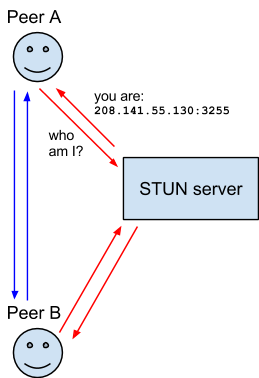
\includegraphics[width=\textwidth,height=60mm]{img/stun.png}
    \caption{Protocolo STUN.}
    \label{figura:stun}
  \end{minipage}
  \hfill
  \begin{minipage}[b]{0.4\textwidth}
    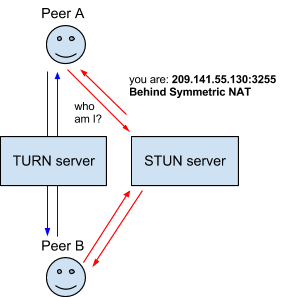
\includegraphics[width=\textwidth,height=60mm]{img/turn.png}
    \caption{Protocolo TURN.}
    \label{figura:turn}
  \end{minipage}
\end{figure}

\item \textbf{SDP} (\textit{Session Description Protocol}) \footnote{\url{https://en.wikipedia.org/wiki/Session_Description_Protocol}}. Es un protocolo empleado para describir una sesión de comunicación multimedia con el fin de anuncio o ode invitación. Su uso predominante se encuentra en el soporte de aplicaciones que utilizan retransmisiones multimedia, como voice over IP (VoIP) y vídeo conferencias.

\end{itemize}

\subsection{Establecimiento de la conexión en WebRTC}
\label{subsec:establecimiento_conexion}

El protocolo WebRTC se encarga de establecer conexiones entre pares, pero desafortunadamente, una conexión WebRTC no se puede establecer sin un servidor intermedio. Este servidor podríamos llamarlo \textbf{servidor de señalización}, empleado en el intercambio de información previo al establecimiento de la conexión WebRTC.

La información que necesitamos intercambiar es una oferta (\textit{Offer}) y una respuesta (\textit{Answer}) que contienen el \textit{Session Description Protocol} mencionado anteriormente en \ref{subsec:protocolos}.

El \textit{Peer A} que inicia la conexión va a crear una oferta. Esta oferta será enviada al par B mediante el servidor intermedio seleccionado. El par B recibirá esta oferta desde el servidor de señalización y creará una respuesta que enviará haciendo uso del mismo intermediario al par A.

\begin{enumerate}
\item Extremo A captura los medios locales mediante \textit{MediaDevices.getUserMedia}

\item Extremo A crea una conexión \textit{RTCPeerConnection} y emplea el método \textit{RTCPeerConnection.addTrack()} para añadir el flujo de datos a la comunicación.

\item Extremo A crea la oferta mediante el método \textit{RTCPeerConnection.createOffer()}.

\item Extremo A establece el SDP de su oferta llamando al método \textit{RTCPeerConnection.setLocalDescription()}.

\item Extremo A solicita al servidor STUN que genere los candidatos ICE.

\item Extremo A usa el servidor de señalización para transmitir su oferta.

\item Extremo B recibe la oferta y emplea \textit{RTCPeerConnection.setRemoteDescription()} para almacenar el SDP del par A.

\item Extremo B hace la configuración necesaria relativa a su conexión, como obtener su flujo de datos multimedia.

\item Extremo B crea una respuesta haciendo uso del método \textit{RTCPeerConnection.createAnswer()}.

\item Extremo B establece su descripción local llamando a \textit{RTCPeerConnection.setLocalDescription()} y pasando la respuesta por parámetro.

\item Extremo B envía la respuesta usando el servidor de señalización.

\item Extremo A recibe la respuesta.

\item Extremo A almacena el SDP del par B llamando al método \textit{RTCPeerConnection.setRemoteDescription()}. Ahora el par A y el par B tienen la configuración de ambos y el flujo de medios comienza a transmitirse.
\end{enumerate}

\subsection{Candidatos ICE}
\label{subsec:candidatos_ice}

Además de intercambiarse la información sobre los elementos multimedia, los pares deben intercambiar información sobre la conexión. Esto es conocido como \textit{candidatos ICE}, que detallan los métodos disponibles con los que un extremo puede comunicarse (directamente o indirectamente mediante un servidor TURN). Cada \textit{peer} propondrá una lista con sus mejores candidatos primero, estos candidatos son UDP (puesto que es más rápido, pues no hay retransmisiones, ni recuperación frente a pérdidas), aunque también permite emplear candidatos TCP. Esta comunicación es transparente para el usuario.

\begin{figure}[H]
	\centering
    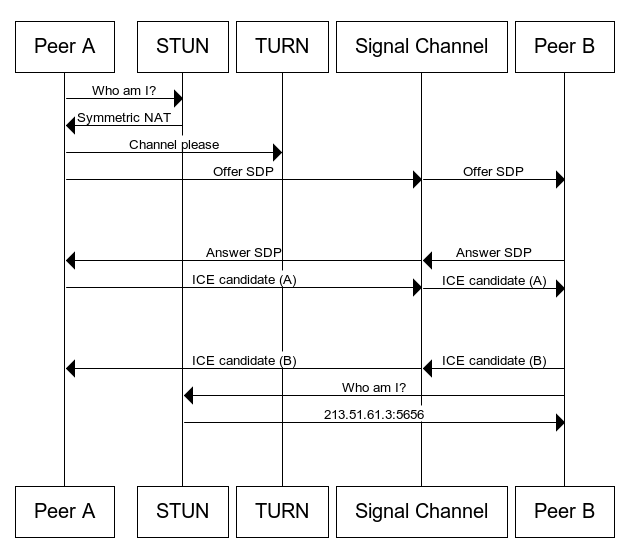
\includegraphics[width=10cm]{img/ice_diagram.png}
    \caption{Diagrama de intercambio de candidatos ICE.}
    \label{figura:nocss_vs_css}
\end{figure}

\section{Control de versiones}
\label{sec:control-de-versiones}

En todo desarrollo de aplicaciones software es necesaria una herramienta de control de versiones que facilite la gestión del código fuente. Estas herramientas realizan un control de todas las modificaciones, de manera que si se comete un error en un determinado instante, se puede volver a una versión anterior del código fuente de la aplicación. La herramienta empleada para el control de versiones en este proyecto es \emph{GitHub}.

Esta herramienta permite clonar cualquier repositorio en nuestra máquina local y mantenerlo actualizado frente a cambios que se hagan en el extremo remoto, además simplifica el ciclo de desarrollo en proyectos grandes, con varios colaboradores, pues se mantiene un código común (que los desarrolladores pueden sincronizar) con la incorporación de modificaciones por parte de los distintos colaboradores. También podemos contribuir en este código realizando parches (\emph{Pull Requests}). Es una herramienta muy potente, lo que le hace ser una de las herramientas de control de versiones más utilizadas internacionalmente por la comunidad de desarrolladores.

\emph{GitHub} proporciona un interfaz gráfico que permite, de manera gráfica, ver la actividad de un repositorio, lo que permite saber si un proyecto tiene una gran cantidad de desarrolladores.

\begin{figure}[H]
	\centering
    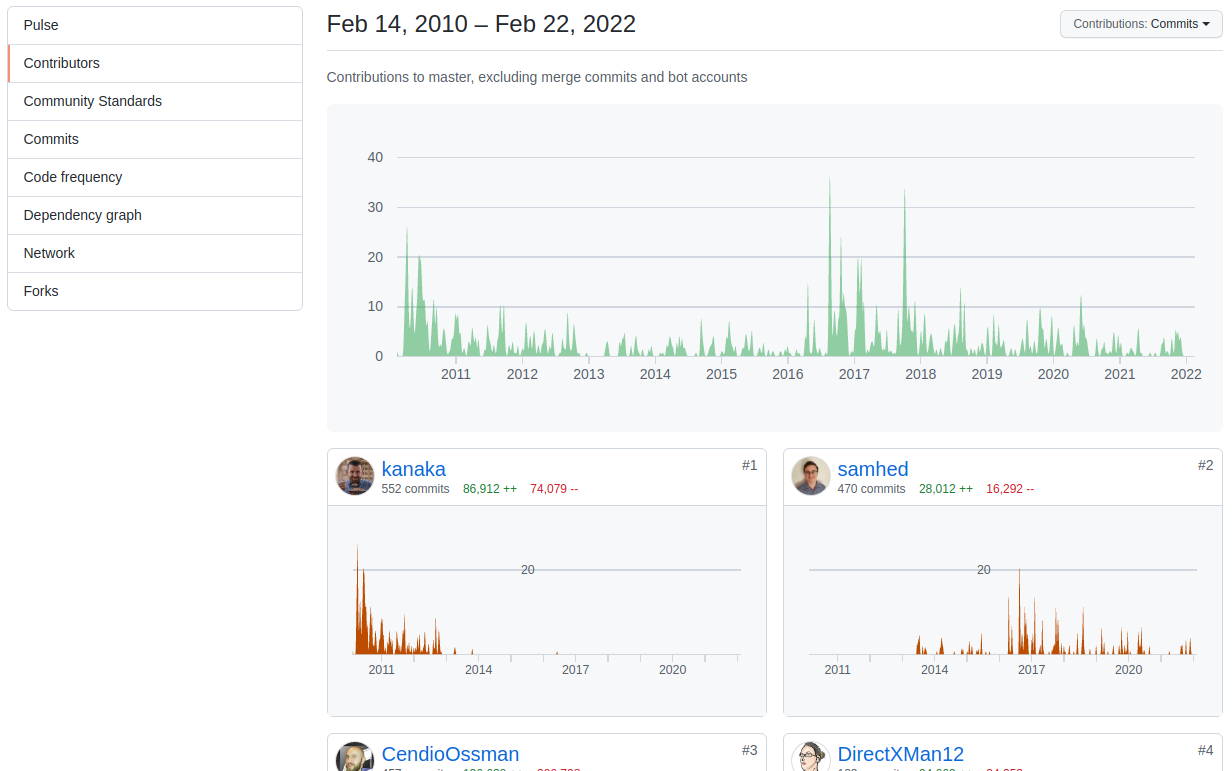
\includegraphics[width=15cm]{img/github_contributors.png}
    \caption{Gráfico de.actividad del repositorio \emph{noVNC} de GitHub.}
    \label{figura:simulador_gazebo}
\end{figure}

\subsection{noVNC}
\label{subsection:novnc}

La herramienta \emph{noVNC} \footnote{https://novnc.com/info.html} es un proyecto de código abierto con un gran número de usuarios, desarrolladores y contribuidores. Esta herramienta ofrece un cliente web VNC construido sobre \emph{JavaScript} y empleando \emph{HTML5}, \emph{WebSockets} y \emph{Canvas}, que funciona en la gran mayoría de navegadores modernos de manera fluida. Incluye un servidor VNC que debe de ejecutarse en la máquina desde la que se quiere compartir el contenido multimedia, y, finalmente desde el cliente web VNC conectarse a este servidor que proporciona el contenido multimedia que será mostrado en el cliente web mediante un elemento \emph{canvas}.

%%%%%%%%%%%%%%%%%%%%%%%%%%%%%%%%%%%%%%%%%%%%%%%%%%%%%%%%%%%%%%%%%%%%%%%%%%%%%%%%
%%%%%%%%%%%%%%%%%%%%%%%%%%%%%%%%%%%%%%%%%%%%%%%%%%%%%%%%%%%%%%%%%%%%%%%%%%%%%%%%
% Robotics Academy %
%%%%%%%%%%%%%%%%%%%%%%%%%%%%%%%%%%%%%%%%%%%%%%%%%%%%%%%%%%%%%%%%%%%%%%%%%%%%%%%%
\section{RoboticsAcademy}
\label{section:roboticsacademy}

RoboticsAcademy \footnote{\url{https://github.com/jderobot/RoboticsAcademy}} es una plataforma de código abierto proporcionada por JdeRobot \footnote{\url{https://github.com/jderobot}}. Esta plataforma ofrece una colección de ejercicios para aprender robótica de una manera práctica. La herramienta principal empleada es un simulador \emph{Gazebo}, el entorno que nos permite visualizar la ejecución de los ejercicios.

\subsection{Arquitectura}

Esta plataforma emplea un servidor \emph{Django} para servir los contenidos, este servidor está contenido dentro del contenedor docker RADI que proporciona. Cada ejercicio se comunica con diferentes componentes del contenedor vía \emph{WebSockets}.

El contenedor docker RADI (Robotics Academy Docker Image) incluye un conjunto de ejercicios que hacen uso de \emph{Gazebo} en su simulación. Para comunicarse con este contenedor desde el lado del navegador web, se accede mediante un \emph{WebSocket} en el puerto 8765, empleando un protocolo de comunicación específico RAMP (Robotics Academy Manager Protocol), mediante esta conexión se mandan las órdenes relativas a la ejecución de los ejercicios. Cada ejercicio abrirá una serie de \emph{WebSockets} adicionales necesarios para que los complementos del ejercicio puedan intercambiar información.

Cada ejercicio está compuesto por una plantilla que muestra el navegador web llamada \emph{exercise.html} y un archivo Python llamado \emph{exercise.py}. El \emph{exercise.py} se ejecuta dentro del contenedor docker RADI, mientras que el \emph{exercise.html} lo muestra el navegador. Ambos se comunican vía \emph{WebSockets} de manera bidireccional.

%%%%%%%%%%%%%%%%%%%%%%%%%%%%%%%%%%%%%%%%%%%%%%%%%%%%%%%%%%%%%%%%%%%%%%%%%%%%%%%%
%%%%%%%%%%%%%%%%%%%%%%%%%%%%%%%%%%%%%%%%%%%%%%%%%%%%%%%%%%%%%%%%%%%%%%%%%%%%%%%%
% UNIBOTICS %
%%%%%%%%%%%%%%%%%%%%%%%%%%%%%%%%%%%%%%%%%%%%%%%%%%%%%%%%%%%%%%%%%%%%%%%%%%%%%%%%
\section{Unibotics}
\label{section:unibotics}

\emph{Unibotics} \footnote{\url{https://unibotics.org/}} es una plataforma que, al igual que RoboticsAcademy, se centra en el aprendizaje de la robótica de manera práctica. Esta plataforma hace uso del RADI de RoboticsAcademy para la ejecucción de los ejercicios, pero no hace uso del servidor local \emph{Django} que contiene el mismo, sino, que ofrece una web en a la que los usuarios pueden acceder desde su navegador, esta plataforma no es de código abierto.

%% IMAGEN DEL RETO FOLLOW LINE
\begin{figure}[H]
	\centering
    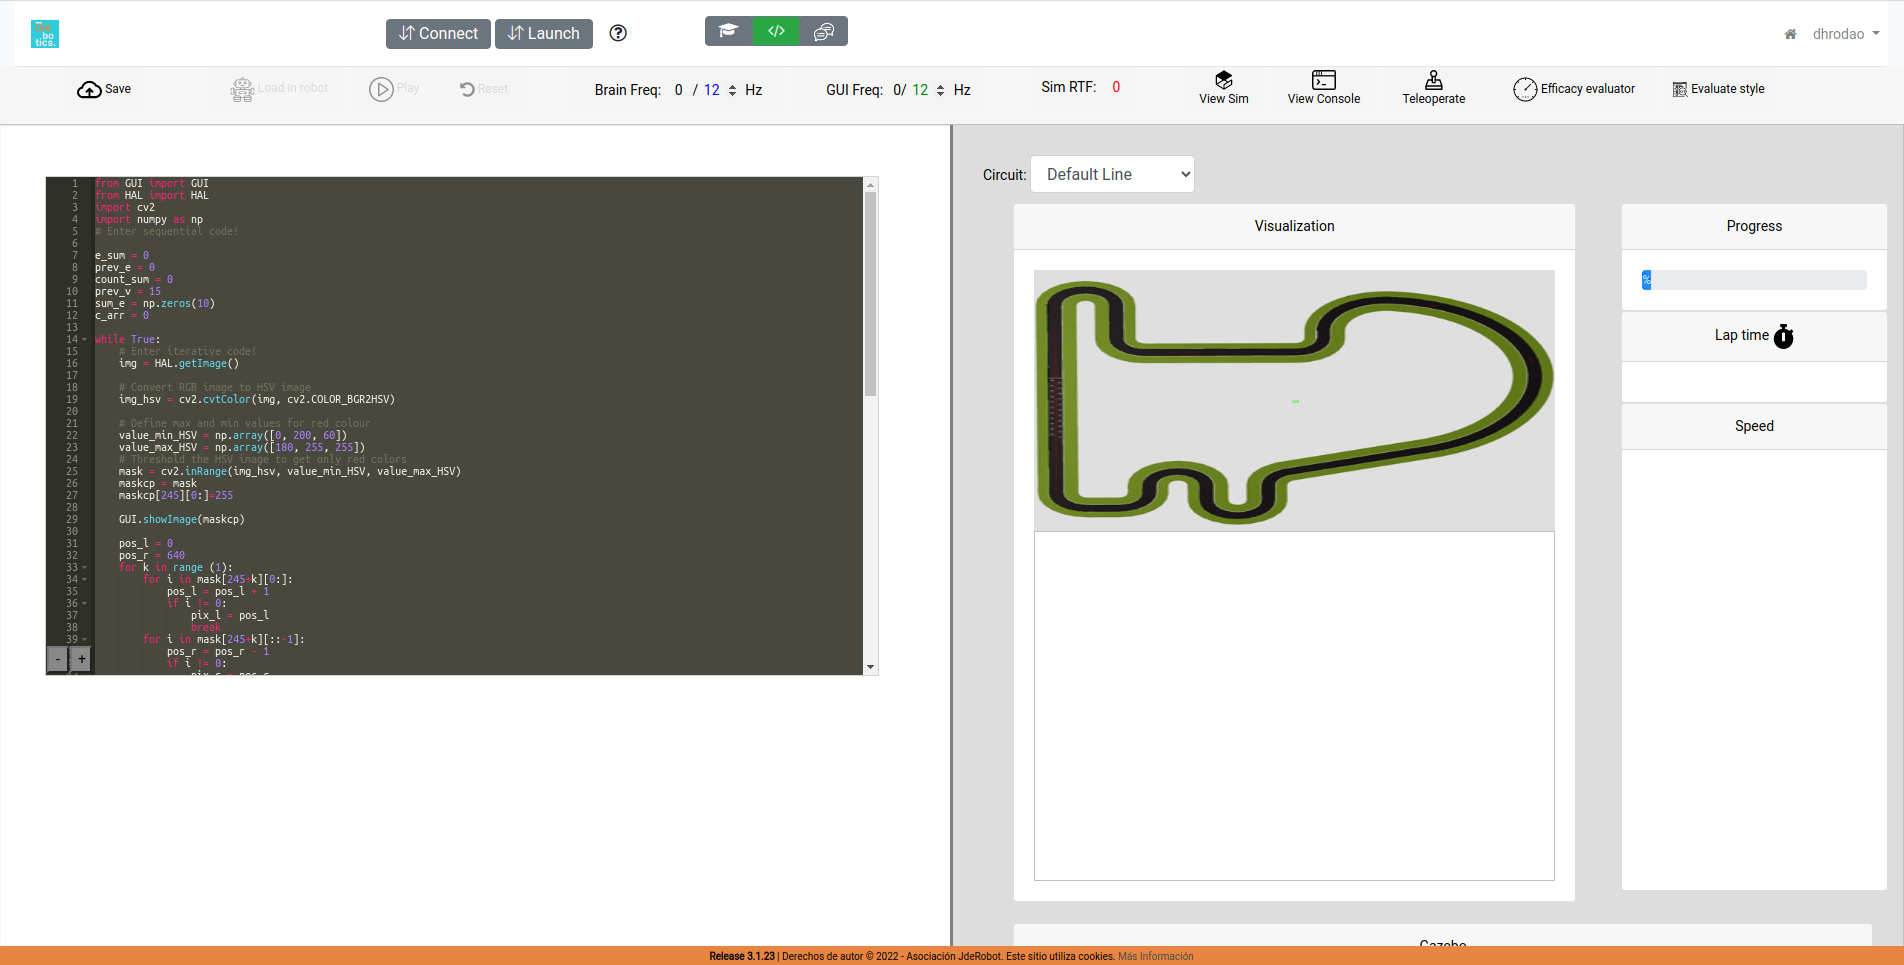
\includegraphics[width=15cm]{img/follow_line.png}
    \caption{Captura del reto Follow Line de Unibotics.}
    \label{figura:unibotics_architecture}
\end{figure}

La arquitectura de la plataforma es muy similar a la de RoboticsAcademy, está formada por tres componentes, un \emph{Webserver}, el \emph{navegador} del usuario y el \emph{RADI} (contenedor Docker donde se ejecutan los ejercicios). A continuación, una descripción del trabajo que realiza cada componente:

\begin{itemize}
\item \textbf{Webserver:} este componente se encarga de proporcionar al navegador del usuario, los componentes del \emph{Front End} que van a ser  necesarios para llevar a cabo la ejecución del ejercicio en cuestión. Proporciona las plantillas \textbf{HTML} y el código \textbf{JavaScript}. También se encarga de almacenar y traer el código del usuario desde \textbf{AWS} (\emph{Amazon Web Services} \footnote{\url{https://es.wikipedia.org/wiki/Amazon_Web_Services}}), con el fin de tener una persistencia del código del mismo.

\item \textbf{Navegador:} ejecuta en la máquina del usuario, es el encargado de comunicarse con el RADI y mostrar toda la información relacionada con la simulación al usuario. Este componente muestra las plantillas de los ejercicios recibidas desde el Webserver al usuario. Mediante \emph{listeners} (escritos en \textbf{JavaScript}) sobre distintos elementos de la plantilla proporciona los controles sobre la ejecución del ejercicio (Play, Reset, Load Code, Gazebo, etc.). Además de proporcionar los controles sobre el ejercicio, también debe de transmitir estas órdenes al contenedor donde se aloja el ejercicio, de manera que durante el establecimiento de la conexión con este, en el caso de los juegos con dos vehículos, se establecen cinco WebSockets. Estos son, un máster, por el que se envían los comandos relacionados con el lanzamiento del ejercicio y Gazebo, y un dos WebSockets por cada vehículo, el primero \emph{ws\_code}, empleado para el envío del código al contenedor, se encarga de interactuar con el cerebro del robot, y, por útlimo, \emph{ws\_gui} cuya función es mostrar toda la información relativa a la interfaz de usuario (mapa al estilo f1, autoevaluador, imágenes de las cámaras), es decir, recibe toda la información del robot.

\item \textbf{RADI:} es uno de los componentes con más peso, pues es donde se ejecuta la simulación. Este ofrece una serie de elementos,  \emph{ws\_manager}, \emph{ws\_code} y \emph{ws\_gui} mencionados anteriormentes, y adicionalmente, ofrece la visualización de Gazebo mediante \emph{GZClient \footnote{\url{http://manpages.ubuntu.com/manpages/bionic/man1/gzclient.1.html}}} y de la consola del contenedor, ambos por medio de un servidor \emph{noVNC \footnote{\url{https://novnc.com/info.html}}} alojado localmente en el contenedor, al cual se conectará el navegador para mostrar dichos elementos.
\end{itemize}

\begin{figure}[H]
	\centering
    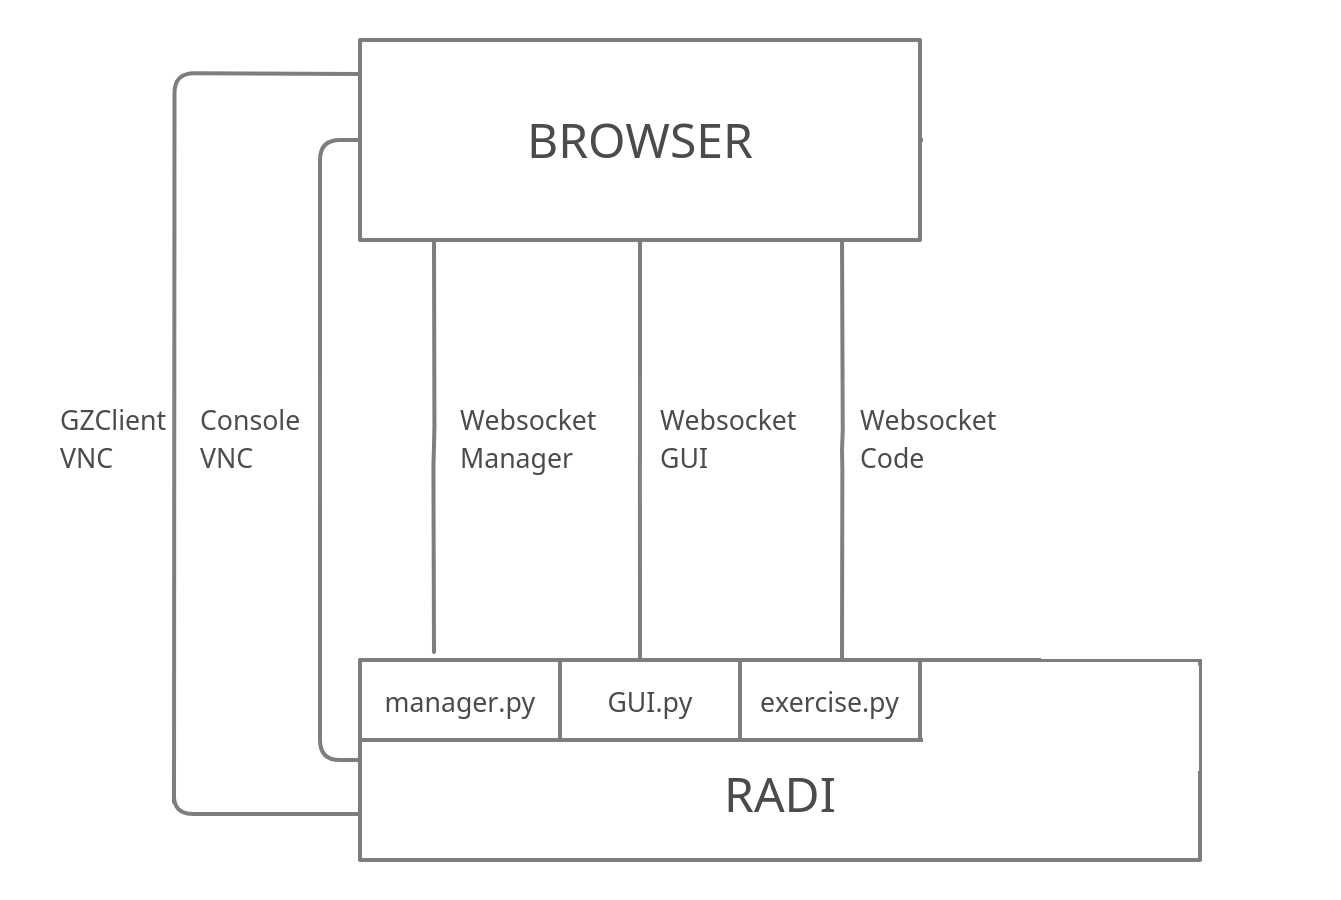
\includegraphics[width=10cm]{img/robotics_academy_architecture.png}
    \caption{Arquitectura de RoboticsAcademy y Unibotics.}
    \label{figura:unibotics_architecture}
\end{figure}


%%%%%%%%%%%%%%%%%%%%%%%%%%%%%%%%%%%%%%%%%%%%%%%%%%%%%%%%%%%%%%%%%%%%%%%%%%%%%%%%
%%%%%%%%%%%%%%%%%%%%%%%%%%%%%%%%%%%%%%%%%%%%%%%%%%%%%%%%%%%%%%%%%%%%%%%%%%%%%%%%
% JUEGOS ASÍNCRONOS %
%%%%%%%%%%%%%%%%%%%%%%%%%%%%%%%%%%%%%%%%%%%%%%%%%%%%%%%%%%%%%%%%%%%%%%%%%%%%%%%%

\cleardoublepage
\chapter{Juegos Asíncronos}

En este capítulo se expondrán los \emph{juegos asícronos} desarrollados para la plataforma de \textit{Unibotics}. Se han desarrollado dos juegos asíncronos, de los que se hablará desde el diseño de las plantillas de la interfaz de usuario, hasta la comunicación con el servidor y el contenedor docker donde es ejecutado el juego, para llevar a cabo el desarrollo de estos juegos, se ha partido de las versiones ya existentes de dos ejercicios individuales dentro de la plataforma.

\section{Diseño de los juegos asíncronos}
\label{sec:async_infraestructura}

Para la realización de los siguientes ejercicios, se ha trabajado sobre la infraestructura inicial en la que opera Unibotics. Ha sido necesario realizar algunas modificaciones de cara a la implementación de los ejercicios, además de añadir nuevas partes. 

Se han desarrollado las siguientes funcionalidades:

\begin{itemize}
\item Interfaz de usuario modificado
\item Evaluadores automáticos
\item Escenarios con dos robots
\item Carga en caliente de código fuente del cerebro de los dos robots
\item Oponentes automáticos: modelos 3D y cerebros
\item \emph{WebSockets} adicionales empleados en la comunicación
\end{itemize}

%\subsection{Interfaz de usuario}

Ha sido necesario hacer una remodelación de las interfaces de usuario en la página web para incorporar el selector de oponentes automáticos, el evaluador automático y de algunos botones y selectores específicos de cada ejercicio.

%\subsection{Evaluadores automáticos}

Para cada ejercicio se ha implementado un evaluador automático haciendo uso de \emph{JavaScript}, con el objetivo de que el usuario que está ejecutando la simulación pueda obtener retroalimentación de cómo está funcionando su robot.

\begin{figure}[H]
	\centering
    \includegraphics[width=18cm]{img/diseño_juegos_asincronos.png}
    \caption{Diseño de arquitectura de los juegos asíncronos.}
    \label{figura:arquitectura_async}
\end{figure}

%\subsection{Escenarios con dos robots}

Para poder implementar los juegos, ha sido necesario realizar primero un estudio sobre aquellos retos en los que tendría sentido implementar una competición.  Para implementar dicha competición es necesario que dos robots puedan actuar simultáneamente en el mismo escenario, y además, que estos puedan realizar algún tipo de duelo. Con este motivo, han sido seleccionados los juegos Follow Line y Drone Cat Mouse para la implementación de un escenario competitivo. En este escenario el usuario tendrá el objetivo de programar un robot para que compita tratando de alcanzar a otro robot dentro de un circuito, o, retar al usuario a que un drone programado por él o ella siga de manera fructuosa a otro drone objetivo.

%\subsection{Carga de código en los robots}

Con la incorporación de un segundo robot al escenario simulado es necesario hacer una modificación en la arquitectura existente del RADI, pues, en un primer lugar, solo había un robot. Ahora, habiendo un segundo, ha sido necesario añadir un controlador para este, que se carga en caliente con el código fuente del cerebro de ese robot. Por este motivo, los \emph{WebSockets} del escenario serán duplicados, puesto que cada robot ha de comunicarse con el navegador web y viceversa. Además, ha sido necesaria la implementación de una nueva interfaz en el servidor web, que escucha peticiones de códigos fuente. Por medio de esta interfaz, el navegador se encargará de hacer las consultas para pedir el código fuente correspondiente. En el lado del servidor web, al recibir una petición en esta interfaz, este se encargará de pedir el código al almacenamiento persistente en S3 (AWS) y enviárselo al navegador web para que se cargue en el robot simulado adecuado.

%\subsection{Oponentes automáticos}

En los juegos asíncronos, el usuario tiene la posibilidad de escoger el oponente automático con el nivel de dificultad a la que quiera enfrentarse. Para que esto sea posible, ha sido necesario implementar una serie de códigos fuente correspondientes a cada nivel de dificultad. Se han creado tres usuarios en la base de datos de \emph{Unibotics} (bot1, bot2, bot3) a los que se asocian los respectivos códigos para cada ejercicio. Una vez un usuario selecciona una dificultad, al cargar el código en los robots, este código se pedirá al servidor web, que este a su vez lo pedirá a AWS (Amazon Web Services), y lo devolverá al navegador. Finalmente, desde el navegador, será enviado al robot correspondiente por medio de su \emph{WebSocket} de código como se muestra en la figura \ref{figura:arquitectura_async}.

%\subsection{WebSockets empleados en la comunicación}

Cada uno de los ejercicios que se han desarrollado emplea una serie de conexiones con el contenedor docker (RADI) con el fin de intercambiar información entre la interfaz de usuario y el contenedor docker (RADI) donde se ejecuta la simulación. Estos WebSockets son:

\begin{itemize}
\item \emph{WebSocket} maestro: entre el navegador web y el manager. Empleado para el control de la ejecución del ejercicio, utiliza un protocolo de mensajes propio de RADI, sirve para lanzar los ejercicios, reanudar la simulación, parar la simulación, etc.
\item \emph{WebSockets} de código: se emplea uno para cada robot del escenario, este canal es empleado para el envío del código fuente Python a los robots que están dentro del simulador desde el lado del navegador.
\item \emph{WebSockets} de interfaz: se emplea uno para cada robot del escenario, este canal es usado para la recepción de datos sensoriales, utilizados para mostrar los datos en la interfaz del usuario, como por ejemplo la posición de los robots, y para la frecuencia de simulación, etc.
\end{itemize}

\section{Juego del Sigue Líneas} 
\label{sec:follow_line_game}

En esta sección se expondrán las distintas partes de la implementación del juego Follow Line describiendo cada uno de los puntos del diseño e incluyendo su validación experimental.

\subsection{Interfaz de usuario}

Se ha diseñado un interfaz de usuario que radica en la simplicidad, sin proporcionar un exceso de controles. La plantilla es común a la mayoría de los ejercicios de la plataforma, y en ella se integran las funcionalidades particulares a cada ejercicio mediante Javascript y HTML5. Todos los ejercicios tienen en común una barra en la parte superior que contiene una serie de botones para realizar la conexión con el contenedor Docker, que es donde se ejecutará todo lo relativo a la simulación del ejercicio. Esta barra horizontal muestra en la Figura \ref{figura:conexion_radi}.

\begin{figure}[H]
	\centering
    
\includegraphics[width=15cm]{img/barra_radi.png}
    \caption{Barra conexión con RADI.}
    \label{figura:conexion_radi}
\end{figure}

Volviendo a la parte específica para este ejercicio, encontramos una segunda barra horizontal donde se encuentran los controles relativos al control de la simulación, visualización, carga de código e información adicional sobre la simulación.

\begin{figure}[H]
	\centering
    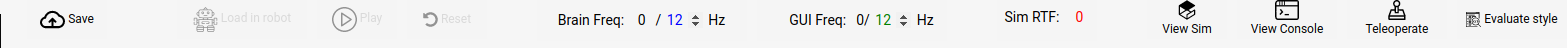
\includegraphics[width=15cm]{img/barra_control.png}
    \caption{Barra de control de la simulación.}
\end{figure}

Bajo las barras de control del ejercicio, se tiene una pantalla que está dividida en dos secciones. La sección izquierda contiene el selector de circuito, el selector de oponente y el editor de código. En la sección derecha se encuentra toda la información que se recibe del escenario, esto es, las localizaciones de los coches y sus cámaras, el evaluador automático, el simulador Gazebo y la consola del contenedor.


\begin{figure}[H]
	\centering
    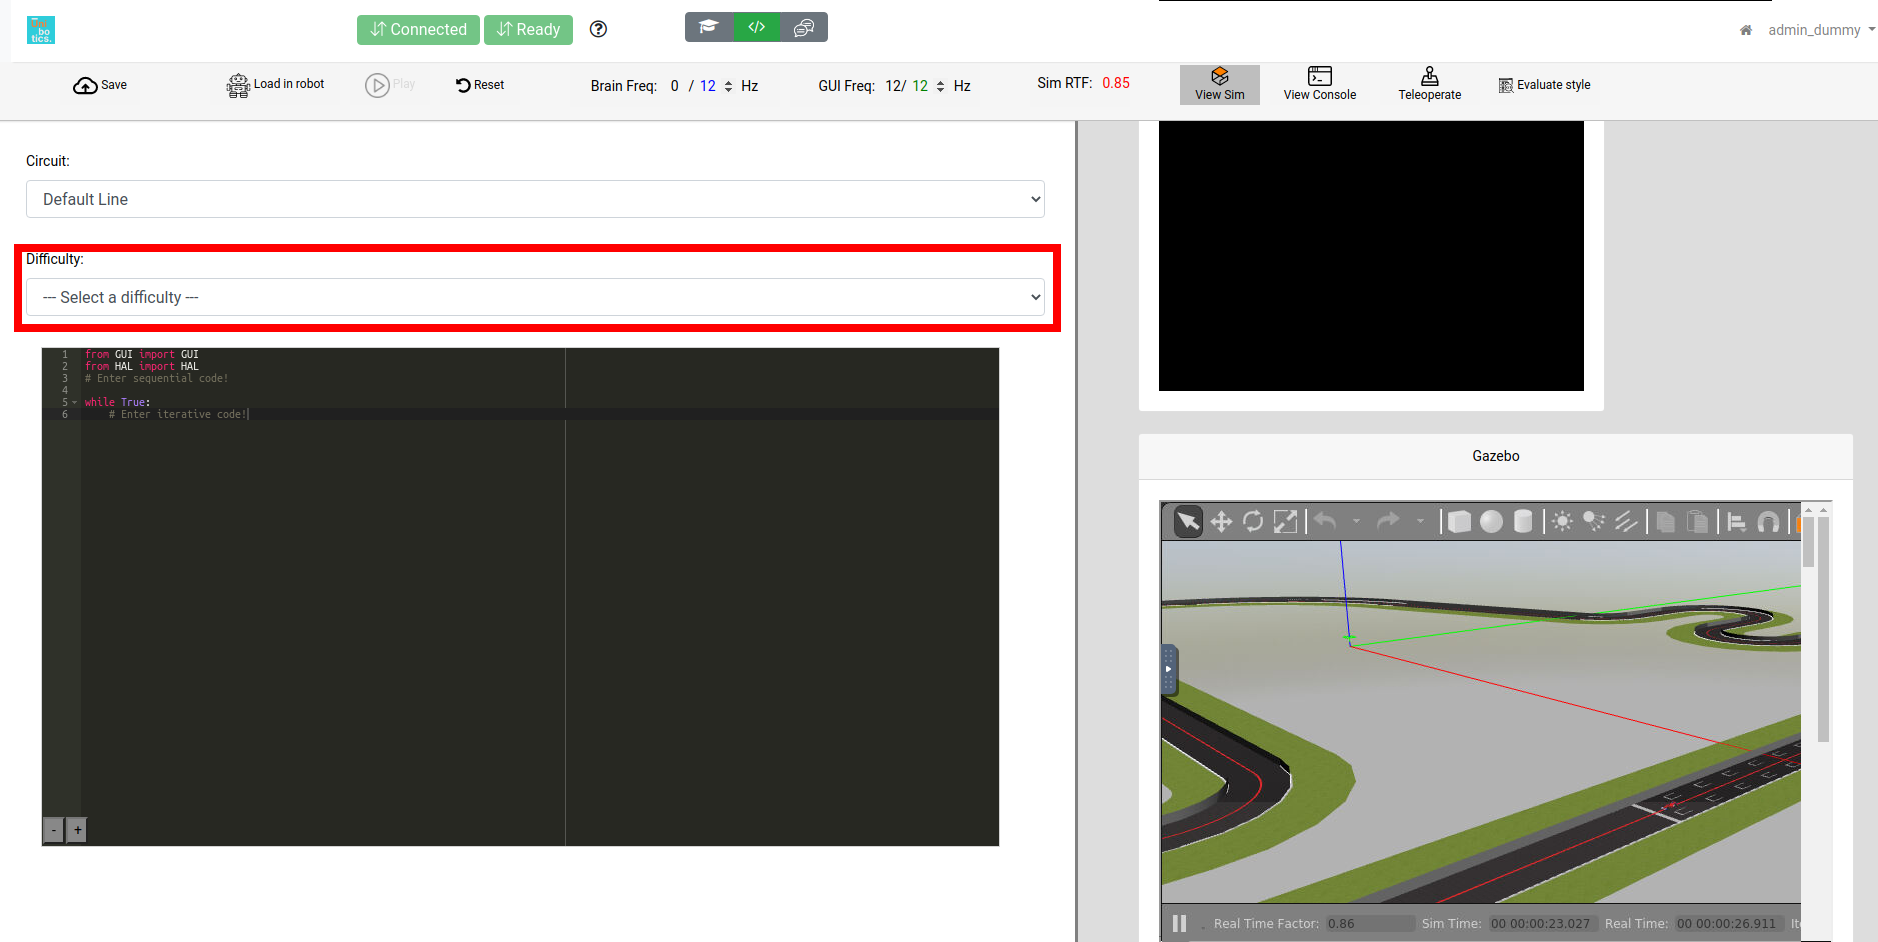
\includegraphics[width=15cm]{img/follow_line_game.png}
    \caption{Plantilla del juego Follow Line. Selector de dificultad explicado con más detalle en \ref{subsec:follow_line_game_difficulty_selector}}
\end{figure}

\subsection{Evaluador automático}
\label{follow_line_game_evaluator}

Este evaluador consiste en mostrar en tiempo real las distancias que hay entre los dos coches, con el fin de que el usuario pueda competir contra el bot automático. A lo largo de cada circuito se han establecido una serie de puntos de control, que sirven para saber en qué lugar se encuentran los robots, y, con esta información calcular la distancia que le queda a cada robot para alcanzar al adversario. Estos \emph{checkpoionts} son almacenados en una serie de \emph{arrays}, y, en función del circuito que haya seleccionado el usuario se emplerá el correspondiente.

La información de posición de los robots se está recibiendo con una determinada frecuencia en el tiempo a través del WebSocket \emph{ws\_gui}, este se encarga de actualizar las variables en la página web que contienen las posiciones de los robots. Se ha desarrollado código JavaScript que se encarga de utilizar los valores que contienen estas variables de posición y calcula el checkpoint más cercano a la posición de cada robot y construye los caminos (\emph{paths}) desde un robot hasta el otro. Una vez se obtienen los paths, se calcula la distancia total de estos y se muestra en la interfaz del usuario.

\begin{figure}[H]
	\centering
    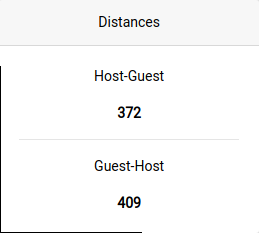
\includegraphics[width=5cm]{img/evaluator_follow_line.png}
    \caption{Interfaz gráfico del evaluador automático.}
    \label{figura:keyhandler}
\end{figure}

\subsection{Robots adversarios: modelo 3D y cerebros}
\label{follow_line_game_adversarios}

Ha sido necesario añadir un nuevo modelo de robot para que el usuario pueda diferenciar entre su robot y el adversario. Para ello simplemente se ha integrado un coche con el mismo modelo que el coche del usuario pero modificando el color. De esta forma, el coche del usuario rojo y el del adversario verde. Esta modificación se ha llevado a cabo usando \emph{Blender} \footnote{\url{https://www.blender.org/}} para modificar el color de las texturas, se ha llamado \emph{f1\_guest}, y ha sido  incluido en el repositorio de la organización \emph{CustomRobots}.

Una vez creado el nuevo modelo, se ha añadido a los ficheros de declaración de los escenarios de Gazebo, incluyendo el nuevo modelo en una posición inicial del circuito en la que ambos coches se encuentran a la misma distancia entre sí. Los ficheros empleados para la configuración del escenario tienen la siguiente forma:

\begin{lstlisting}[basicstyle=\ttfamily\scriptsize]
<?xml version="1.0" ?>
<sdf version="1.5">
  <world name="default">
    <gui fullscreen=1></gui>
    <scene>
      <grid>false</grid>
      <sky>
        <clouds>
          <speed>12</speed>
        </clouds>
      </sky>
    </scene>
    <!-- A global light source -->
    <include>
      <uri>model://sun</uri>
      <name>sun_1</name>
      <pose>0 0 1 0 0 0</pose>
    </include>
    <include>
	    <uri>model://simple_circuit</uri>
	    <pose>0 0 0 0 0 0</pose>
    </include>
    <include>
      <uri>model://f1</uri>
      <pose>53.462 -10.734 0.004 0 0 -1.57</pose>
    </include>
    <include>
      <uri>model://f1_guest</uri>
      <pose>-53.2 -6.8 0.004 0 0 -4.85</pose>
    </include>
  </world>
</sdf>
\end{lstlisting}

Para este juego, han sido implementados tres códigos diferentes que se corresponden con las tres dificultades proporcionadas por la plataforma, finalmente han sido cargados en el juego Follow Line de los correspondientes perfiles creados para la gestión de las dificultades. La dificultad se corresponde con la velocidad que alcanzará el robot adversario, a mayor dificultad, mayor velocidad.

\begin{lstlisting}[basicstyle=\ttfamily\scriptsize]
from GUI import GUI
from HAL import HAL
import cv2
import numpy as np
# Enter sequential code!

e_sum = 0
prev_e = 0
count_sum = 0
prev_v = 15
sum_e = np.zeros(10)
c_arr = 0

while True:
    # Enter iterative code!
    img = HAL.getImage()
    
    # Convert RGB image to HSV image
    img_hsv = cv2.cvtColor(img, cv2.COLOR_BGR2HSV)
    
    # Define max and min values for red colour
    value_min_HSV = np.array([0, 200, 60])
    value_max_HSV = np.array([180, 255, 255])
    # Threshold the HSV image to get only red colors
    mask = cv2.inRange(img_hsv, value_min_HSV, value_max_HSV)

    GUI.showImage(img)
    
    pix_r = None
    pix_l = None
    pos_l = 0
    pos_r = 640
    for k in range (1):
        for i in mask[256+k][0:]:
            pos_l = pos_l + 1
            if i != 0:
                pix_l = pos_l
                break
        for i in mask[256+k][::-1]:
            pos_r = pos_r - 1
            if i != 0:
                pix_r = pos_r
                break
    
    center = 320
    if (pix_r != None) and (pix_l != None):
        red_center = (pix_r + pix_l)/2
    else:
        red_center = (pos_r + pos_l)/2
    

    e = red_center - center
    
    ### ARRAY SUMA DE ERRORES ANTERIORES ###
    if c_arr<10:
        sum_e[c_arr] = e
    else:
        c_arr = 0;
        sum_e[c_arr] = e
    c_arr += 1
    mean = 0
    for i in range(0,9):
        mean += sum_e[i]
    ########################################
        
    ### CONTROLADOR PID GIRO ###
    kps = -0.003
    kis = -0.00017
    kds = -0.006
    steerSpeed = kps*e+kds*(e-prev_e)+kis*mean
    ############################
    
    ### DETECTOR DE CURVA ###
    count = 0
    for k in range (6):
        for i in mask[256+k][0:300]:
            if i != 0:
                count += 1
        for i in mask[256+k][340:]:
            if i != 0:
                count += 1
    #########################
    
    ### CONTROLADOR VELOCIDAD ###
    kdv = 0.046
    kiv = 0.0022
    forwardSpeed = 5 - kdv*count - kiv*abs(mean)
    #print(forwardSpeed, steerSpeed, count)
    #################################
    
    HAL.setV(forwardSpeed)
    HAL.setW(steerSpeed)
    
    count_sum = count_sum + 1
    prev_e = e
\end{lstlisting}

\subsection{Carga de código del cerebro del robot}
\label{follow_line_game_code_load}

Una vez se ha establecido la conexión de \emph{RADI} con el navegador, se puede proceder a la carga del código. Esta carga se realiza mediante un botón \emph{Load in robot}, que una vez pulsado, se encarga de habilitar el botón \emph{Play} después de haber realizado una comprobación exitosa del código del usuario.

Cuando el usuario procede a realizar la carga del código en los respectivos robots, el código que ha desarrollado el usuario
se obtiene del editor de código situado en la parte izquierda de la pantalla. Para realizar la carga de código de uno de los bots, se ha desarrollado un script en \emph{JavaScript} que se encarga de realizar una solicitud al servidor web, pidiendo el código correspondiente con la dificultad seleccionada.

Para que el servidor web pueda proporcionar el código de cada dificultad al navegador web solicitante, se han creado una serie de usuarios instrumentales con el prefijo de \emph{bot}, que contienen el código correspondiente a cada dificultad. También ha sido necesaria la creación de una nueva ruta (\emph{endpoint}) en el servidor web. Desde el lado del servidor web, cuando se recibe una solicitud en dicha interfaz, este se encarga de determinar cuál es la dificultad y el ejercicio del que se está solicitando por medio de los datos aportados en la propia cadena de búsqueda.

Finalmente, una vez se tienen ambos códigos fuente, estos se envían cada uno por el \emph{WebSocket} de código que se corresponde con cada robot del escenario, de manera que el código será recibido en el contenedor docker (RADI), procesado, e insertado en el cerebro de cada robot dentro del simulador. 

\subsubsection{Inicio del juego}
\label{subsec:follow_line_game_inicio}

Para iniciar el juego es necesario realizar previamente la conexión con el contenedor Docker (\emph{RADI}) donde se va a llevar a cabo toda la ejecución del ejercicio. Una vez realizada esta conexión, se deberá seleccionar el circuito concreto en el que el usuario quiere jugar, seleccionar la dificultad del oponente, y, pulsar el botón \emph{Load in robot}, una vez se hayan cargado los respectivos códigos, se podrá proceder pulsando el botón \emph{Play} para comenzar la ejecución.

Con respecto a las versiones iniciales del reto \emph{Follow Line} de Unibotics, ha sido necesaria la programación dentro del contenedor RADI, de la infraestructura que lanza la simulación del ejercicio con el circuito seleccionado por el usuario.

Para implementar esta característica, dentro del fichero \emph{manager.py} (encargado del lanzamiento de los ejercicios, comprobar el código mediante PyLint, noVNC, etc), se ha añadido una variable con ámbito global dentro del fichero \emph{manager.py} que contiene una lista con todos los ejercicios que implementan la funcionalidad de cambio de circuito. De manera que, cuando el contenedor docker recibe una orden de lanzar un ejercicio, previamente al lanzamiento se comprueba si el ejercicio a lanzar implementa dicha funcionalidad, y, si es así, se obtiene el nombre del circuito seleccionado de los datos que se han recibido por este canal de comunicación (el \emph{WebSocket maestro entre el RADI y el navegador}). Una vez obtenido el nombre del circuito que desea lanzar el usuario, se procede a arrancar la simulación Gazebo con el escenario correspondiente al circuito seleccionado.

Finalmente, se lanzará este proceso (además de algunos otros como noVNC para mostrar GZClient y la consola), y se avisará al \emph{Front End} que la conexión está lista.

\subsubsection{Selección de circuito}
\label{subsec:follow_line_game_circuito}

El usuario podrá elegir mediante un desplegable en la página web uno de los circuitos disponibles para realizar la ejecución del juego, estos circuitos son \emph{Default}, \emph{Montmelo}, \emph{Montreal} y \emph{Nürbugring}. 

\begin{figure}[H]
	\centering
    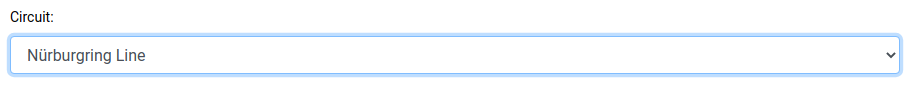
\includegraphics[width=15cm]{img/circuit_selector.png}
    \caption{Selector de circuitos.}
    \label{figura:circuit_selector}
\end{figure}

%\begin{figure}[H]
%	\centering
%    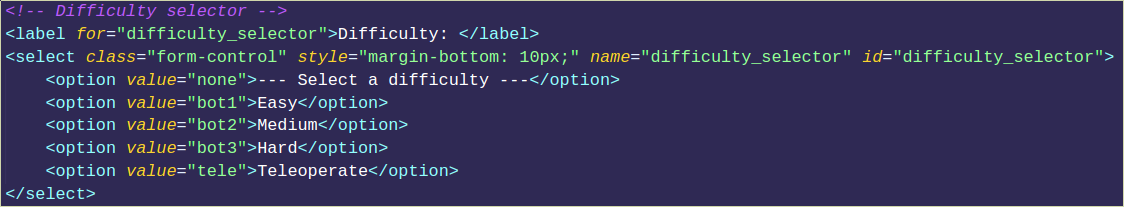
\includegraphics[width=15cm]{img/difficulty_selector_html.png}
%    \caption{Código HTML para la implementación del selector de dificultad.}
%    \label{figura:circuit_selector}
%\end{figure}

\begin{lstlisting}[basicstyle=\scriptsize\ttfamily]
<label for="difficulty_selector">Difficulty: </label>
<select class="form-control" style="margin-bottom: 10px;" name="difficulty_selector" id="difficulty_selector">
	<option value="none">--- Select a difficulty ---</option>
	<option value="bot1">Easy</option>
	<option value="bot2">Medium</option>
	<option value="bot3">Hard</option>
	<option value="tele">Teleoperate</option>
</select>
\end{lstlisting}


El circuito \emph{Default} será el escenario por defecto en el que comenzará la simulación, si el usuario selecciona otro, se le comunicará al contenedor Docker, y este se encargará de volver a lanzar la simulación con el escenario seleccionado. Esta comunicación se realiza por medio de WebSockets.

%\begin{figure}[H]
%	\centering
%    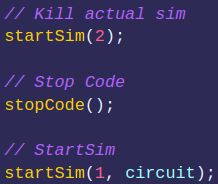
\includegraphics[width=5cm]{img/select_circuit_code.png}
%    \caption{Cambio de circuito.}
%    \label{figura:circuit_change_code}
%\end{figure}

\begin{lstlisting}[basicstyle=\ttfamily\scriptsize]
// Set variable to toggle gazebo
gazeboToggle = true;
// Kill actual sim
startSim(2)
// StartSim
swapping = true;
startSim(1, circuit, "{{websocket_address}}","{{server}}", "{{user.username}}");
connectionUpdate({connection: 'exercise', command: 'swap'}, '*');
firstCodeSent = false;
\end{lstlisting}

Como se puede apreciar en la Figura \ref{figura:circuit_change_code}, el código del selector de circuitos se encarga de matar la simulación en curso e iniciar la nueva simulación con el circuito que se obtiene del selector.

\subsection{Selección de oponente automático}
\label{subsec:follow_line_game_difficulty_selector}

El selector de circuitos brinda al usuario un total de tres oponentes automáticos de dificultades diferentes, \emph{Easy}, \emph{Medium} y \emph{Hard}. Adicionalmente, el usuario también podrá seleccionar una cuarta opción, llamada \emph{Teleoperate} que consiste en que podrá teleoperar el coche del oponente con las teclas de dirección.

\begin{figure}[H]
	\centering
    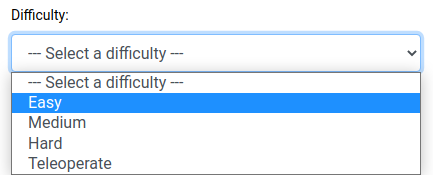
\includegraphics[width=10cm]{img/difficulty_selector.png}
    \caption{Selector de dificultad.}
    \label{figura:difficulty_selector}
\end{figure}

\subsubsection{Modo teleoperado}
\label{follow_line_game_mode_teleoperado}

En este juego se ha considerado el extra de implementar un modo de teleoperación manual para ambos vehículos, para brindar al usuario la posibilidad de probar su código ante diversas situaciones y pueda desarrollar un código más robusto, también con el objetivo de que pueda controlar alguno de los dos vehículos en el caso de que se haya quedado atascado. El usuario podrá controlar su vehículo, mediante el botón de teleoperación situado en la barra superior, y el coche oponente seleccionando la dificultar \emph{Teleoperate}, como se ha mencionado antes.

\begin{figure}[H]
  \centering
  \begin{minipage}[b]{0.4\textwidth}
    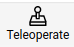
\includegraphics[width=\textwidth,height=\textwidth]{img/teleoperate_off.png}
    \caption{Teleoperación apagada.}
    \label{figura:stun}
  \end{minipage}
  \hfill
  \begin{minipage}[b]{0.4\textwidth}
    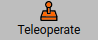
\includegraphics[width=\textwidth,height=\textwidth]{img/teleoperate_on.png}
    \caption{Teleoperación encendida.}
    \label{figura:turn}
  \end{minipage}
\end{figure}

Como se puede apreciar en las Figuras \ref{figura:stun} y \ref{figura:turn}, el botón de teleoperación del vehículo del usuario, cambiará de color en función de si la teleoperación está encendida o apagada.

\subsubsection{Implementación del botón de teleoperación}
\label{follow_line_game_mode_teleoperado_impl}

La teleoperación se ha implementado mediante código JavaScript, con un \emph{listener} para el botón de teleoperación, que se encarga de comprobar si se puede activar el modo, es decir, no se está teleoperando el otro vehículo, cambiar la imagen del botón de teleoperación y añadir el \emph{handler} correspondiente a los eventos \emph{keyup} y \emph{keydown}. A continuación se adjunta un fragmento del código empleado para desarrollar el \emph{listener} del botón de teleoperación:

%\begin{figure}[H]
%	\centering
%    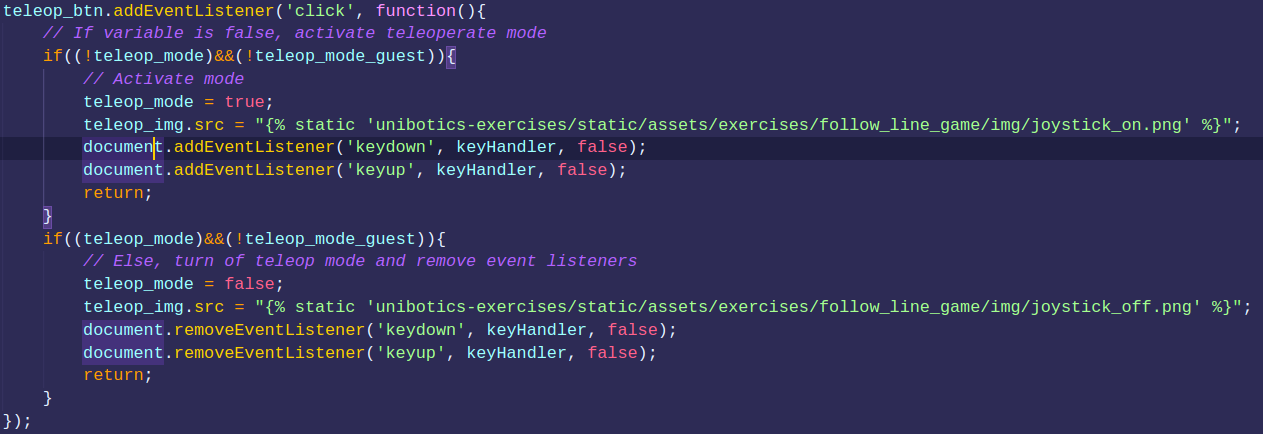
\includegraphics[width=17cm]{img/teleop_mode_code.png}
%    \caption{Listener del botón de teleoperación.}
%    \label{figura:difficulty_selector}
%\end{figure}

\begin{lstlisting}[basicstyle=\ttfamily\scriptsize]
teleop_btn.addEventListener('click', function(){
			// If variable is false, activate teleoperate mode
			if(!teleop_mode){
				if (running == false) {
					resumeSimulation();
					running == true;
				}
				// Activate mode
				teleop_mode = true;
				teleop_btn.style.background = '#BEBEBE';
				teleop_img.src = "";
				document.addEventListener('keydown', keyHandler, false);
				document.addEventListener('keyup', keyHandler, false);
				return;
			}

			// Else, turn of teleop mode and remove event listeners
			teleop_mode = false;
			submitCode();
			teleop_btn.style.background = 'transparent';
			teleop_img.src = "";
			document.removeEventListener('keydown', keyHandler, false);
			document.removeEventListener('keyup', keyHandler, false);
			return;
		});
\end{lstlisting}

El \emph{handler} que se le asigna a los eventos \emph{keyup} y \emph{keydown} se encarga de determinar cual es la tecla que se ha soltado o pulsado, y, si es una de las flechas de dirección establece un valor constante a la variable de velocidad o giro.

\begin{lstlisting}[basicstyle=\ttfamily\scriptsize]
function keyHandler(event) { // Right (39), Left (37), Down (40), Up (38)
		if((typeof(websocket_gui) !== 'undefined' && (typeof(websocket_code) !== 'undefined'))){
			let cmd = "#tele";

			// Prevent using arrow keys to scroll page
			if([32, 37, 38, 39, 40].indexOf(event.keyCode) > -1) {
				event.preventDefault();
			}

			if(event.keyCode == 39) {
				//console.log('Right');
				w = (event.type == 'keydown')?-1:0;
			}else if(event.keyCode == 37) {
				//console.log('Left');
				w = (event.type == 'keydown')?1:0;
			}else if(event.keyCode == 40) {
				//console.log('Down');
				v = (event.type == 'keydown')?-2:0;
			}else if(event.keyCode == 38) {
				//console.log('Up');
				v = (event.type == 'keydown')?2:0;
			}
			console.log('v: ', v, 'w: ', w);
		}
}
\end{lstlisting}

%\begin{figure}[H]
%	\centering
%    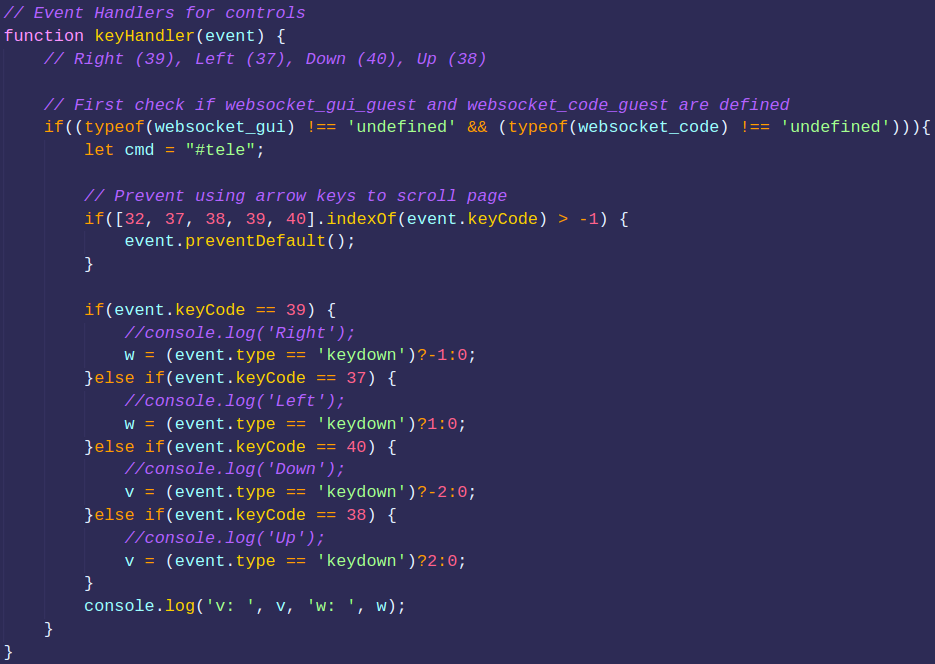
\includegraphics[width=10cm]{img/keyhandler.png}
%    \caption{Key Handler.}
%    \label{figura:keyhandler}
%\end{figure}

Como se puede apreciar en la Figura \ref{figura:difficulty_selector}, los valores de velocidad son asignados a las correspondientes variables de velocidad o de giro. Los valores de estas variables son enviados al contenedor Docker mediante el websocket por el que viaja el código desde el navegador al contenedor.

\subsection{Validación experimental}

En esta sección se describen detalles sobre la ejecución típica del ejercicio, entrando en detalle en todos los pasos que el usuario debe realizar previamente detallados en las secciones anteriores. Con esto se valida el buen funcionamiento del software desarrollado.

En primer lugar, el usuario ha de conectar el navegador con el contenedor docker RADI.

\begin{figure}[H]
	\centering
    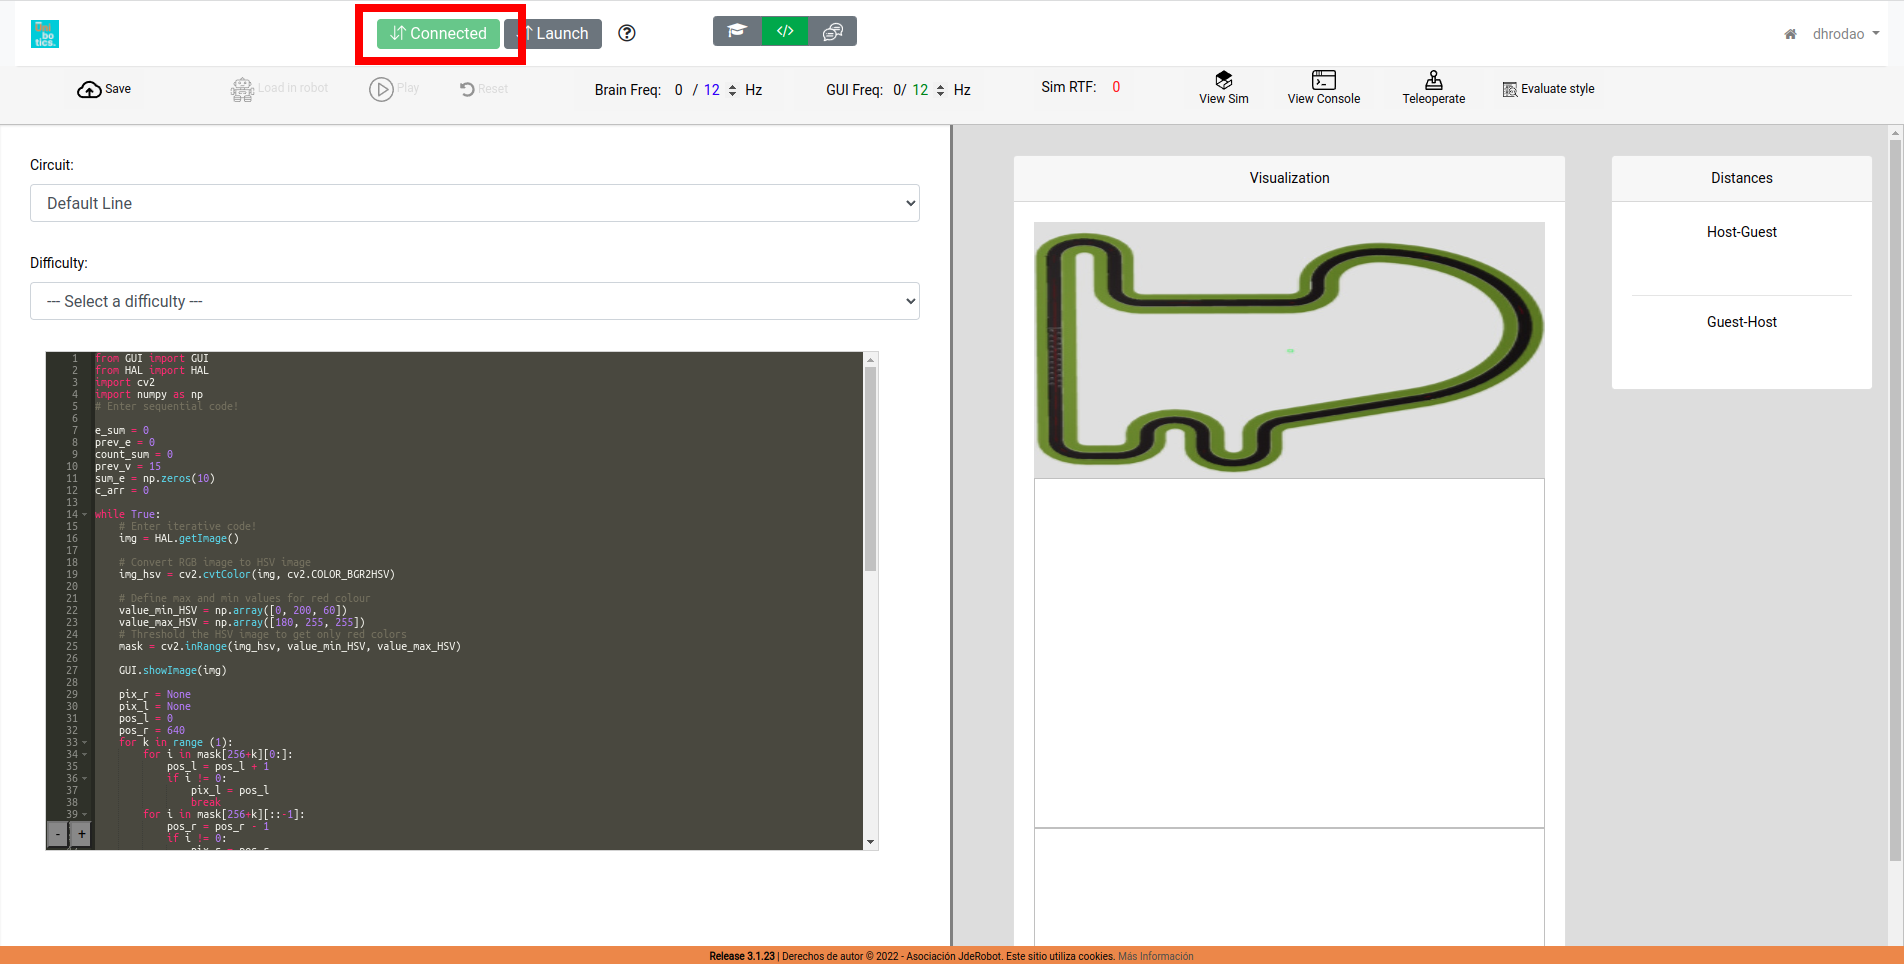
\includegraphics[width=\textwidth]{img/fl_radi_connected_rect.png}
    \caption{Juego Follow Line conectado con RADI.}
    \label{figura:evaluator_drone}
\end{figure}

A continuación, una vez se ha conectado el navegador con RADI, se debe lanzar el ejercicio mediante el botón Launch de la parte superior izquierda de la pantalla.

\begin{figure}[H]
	\centering
    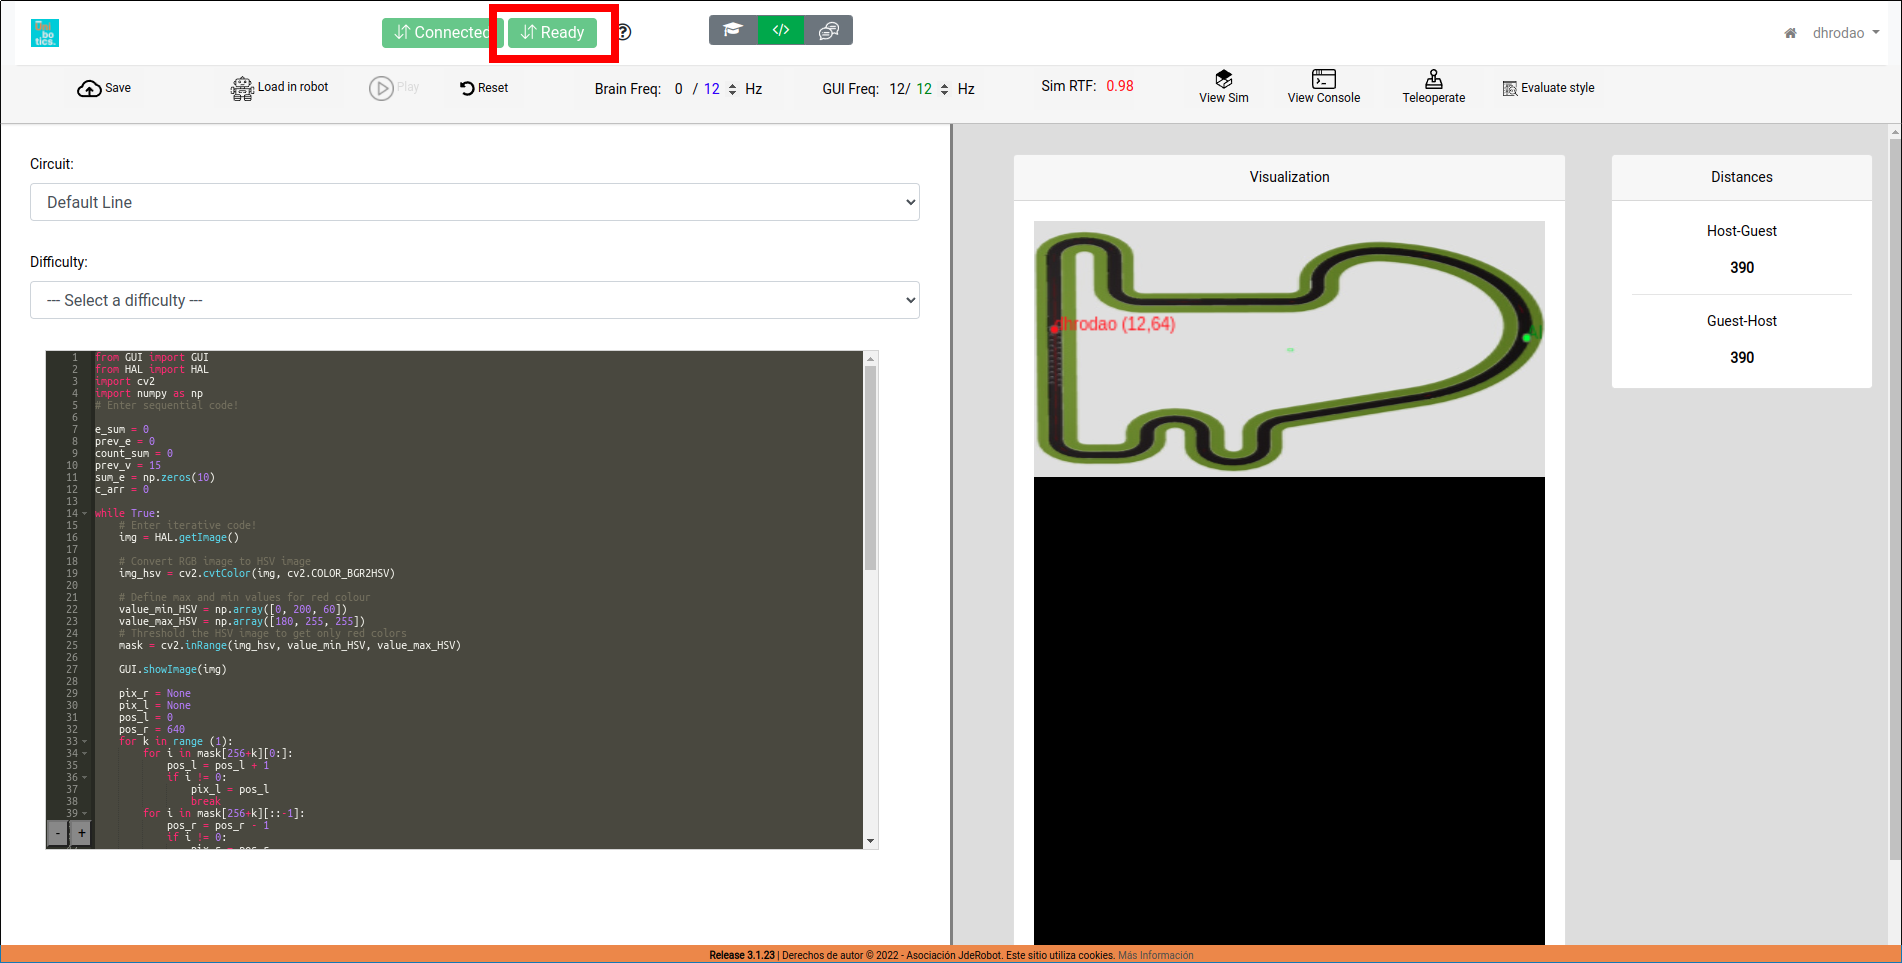
\includegraphics[width=\textwidth]{img/fl_connection_established_rect.png}
    \caption{Juego Follow Line lanzado.}
\end{figure}

Una vez lanzado el ejercicio, se puede proceder a seleccionar un circuito y un oponente automático, para luego cargar el código fuente del robot propio e iniciar la simulación. También se abre \emph{Gazebo} para visualizar el escenario de simulación y la consola. Y finalmente, iniciar la ejecución del juego.

\begin{figure}[H]
	\centering
    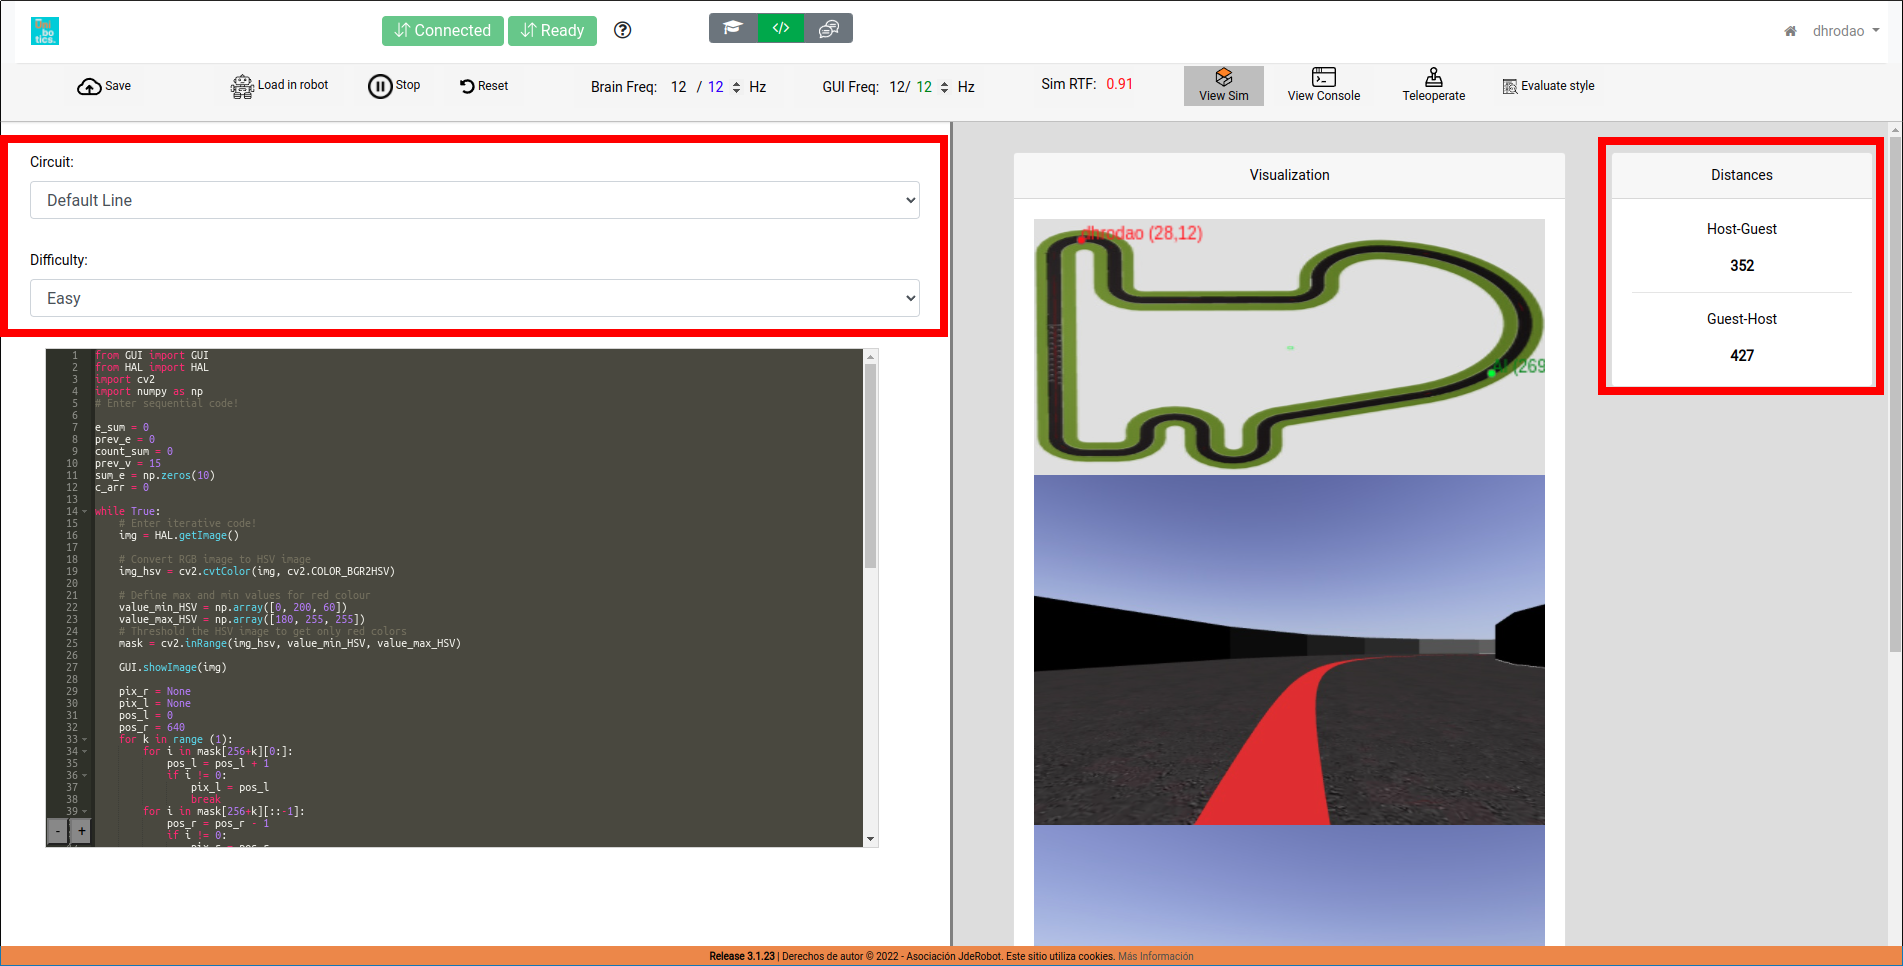
\includegraphics[width=\textwidth]{img/fl_sim_1_rect.png}
    \caption{Evaluadores en la ejecución del juego Follow Line.}
\end{figure}

\begin{figure}[H]
	\centering
    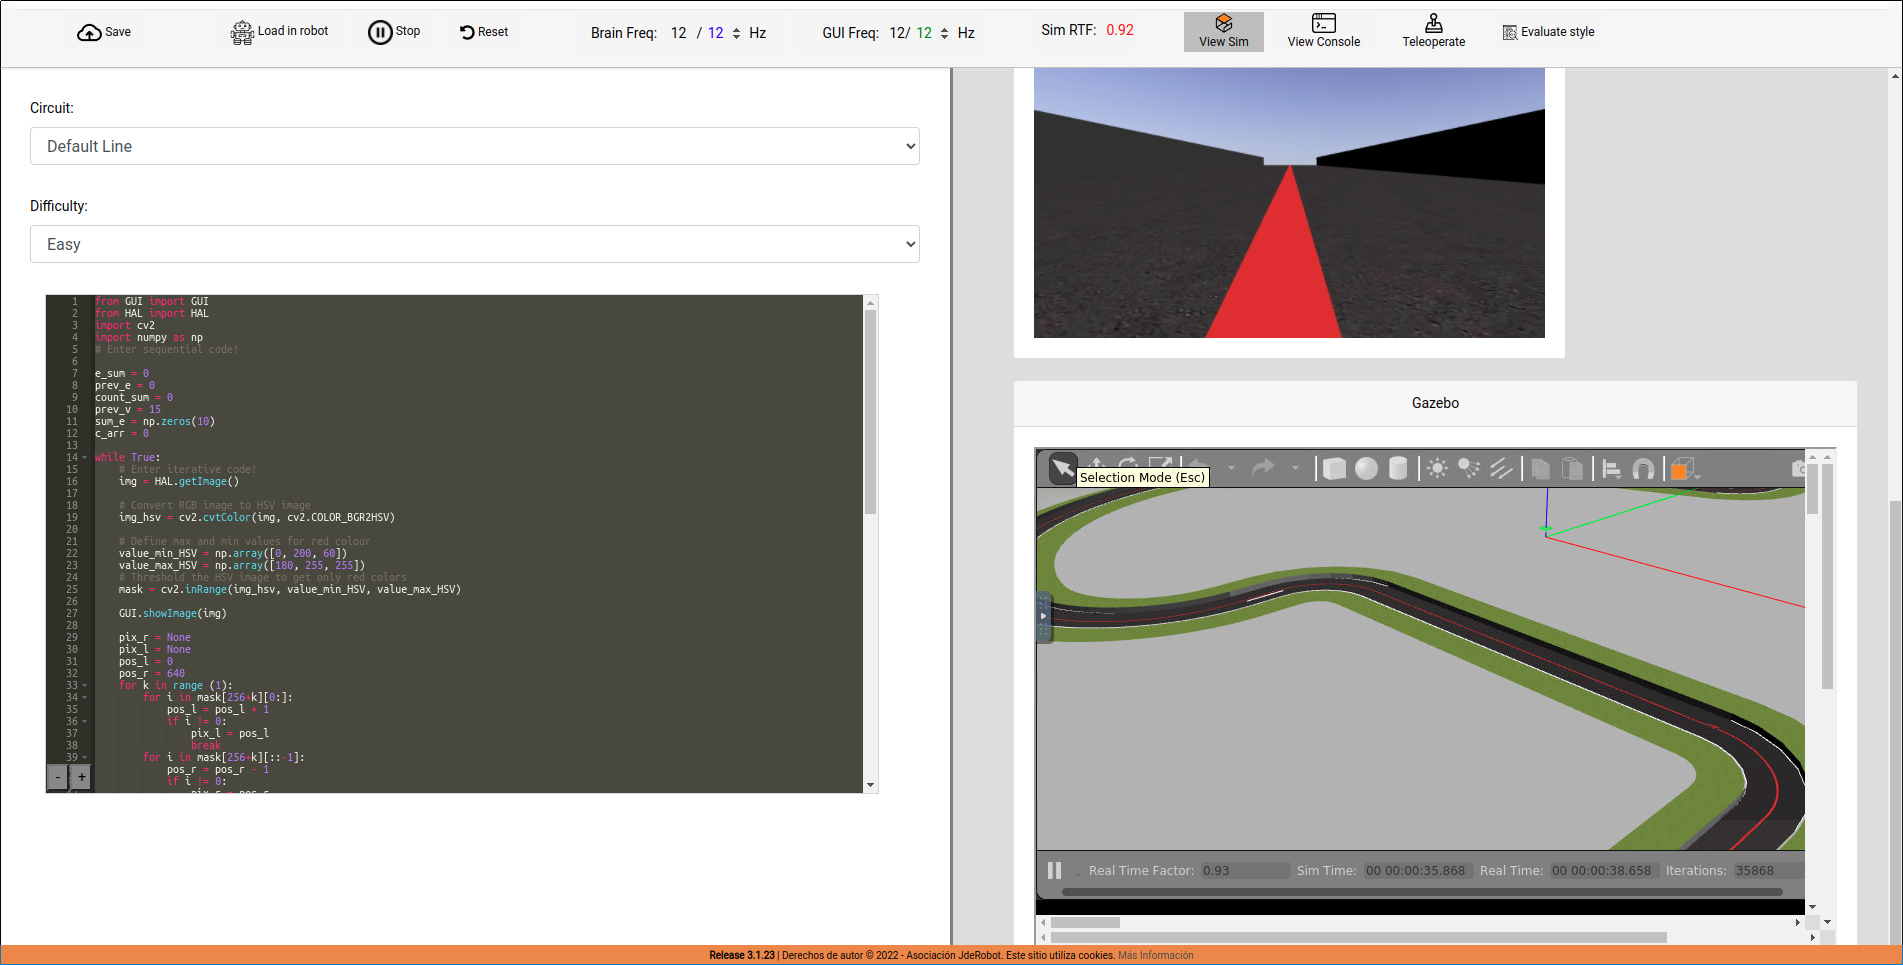
\includegraphics[width=\textwidth]{img/fl_sim_2.png}
    \caption{Simulador en la ejecución del juego Follow Line.}
\end{figure}

Con el objetivo de una mejor comprensión del funcionamiento del juego se ha elaborado un vídeo con un ejemplo más ilustrativo. Está accesible en YouTube en el enlace \textbf{\url{https://www.youtube.com/watch?v=3nWpbP-5lRc}}.

\section{Juego del Gato Ratón con Drones} 
\label{sec:drone_cat_mouse_game}

En esta sección se expondrán las distintas partes de la implementación del juego Drone Cat Mouse describiendo cada uno de los puntos del diseño e incluyendo su validación experimental.

\subsection{Interfaz de usuario}
\label{drone_cat_mouse_interface}

Al igual que todos los juegos de la plataforma, estos comparten una plantilla \emph{HTML} con los componentes básicos de un ejercicio, por lo que para el caso de este ejercicio, cabe mencionar que las barras superiores de conexión con \emph{RADI} y de control de la simulacón son similares a las de Follow Line Game.

Bajo el navbar, a mano izquierda se encuentra el editor de código, y a mano derecha, los botones para el control de la ejecución del ratón, el evaluador automático, el simulador \emph{Gazebo} y la consola del contenedor Docker.


\begin{figure}[H]
	\centering
    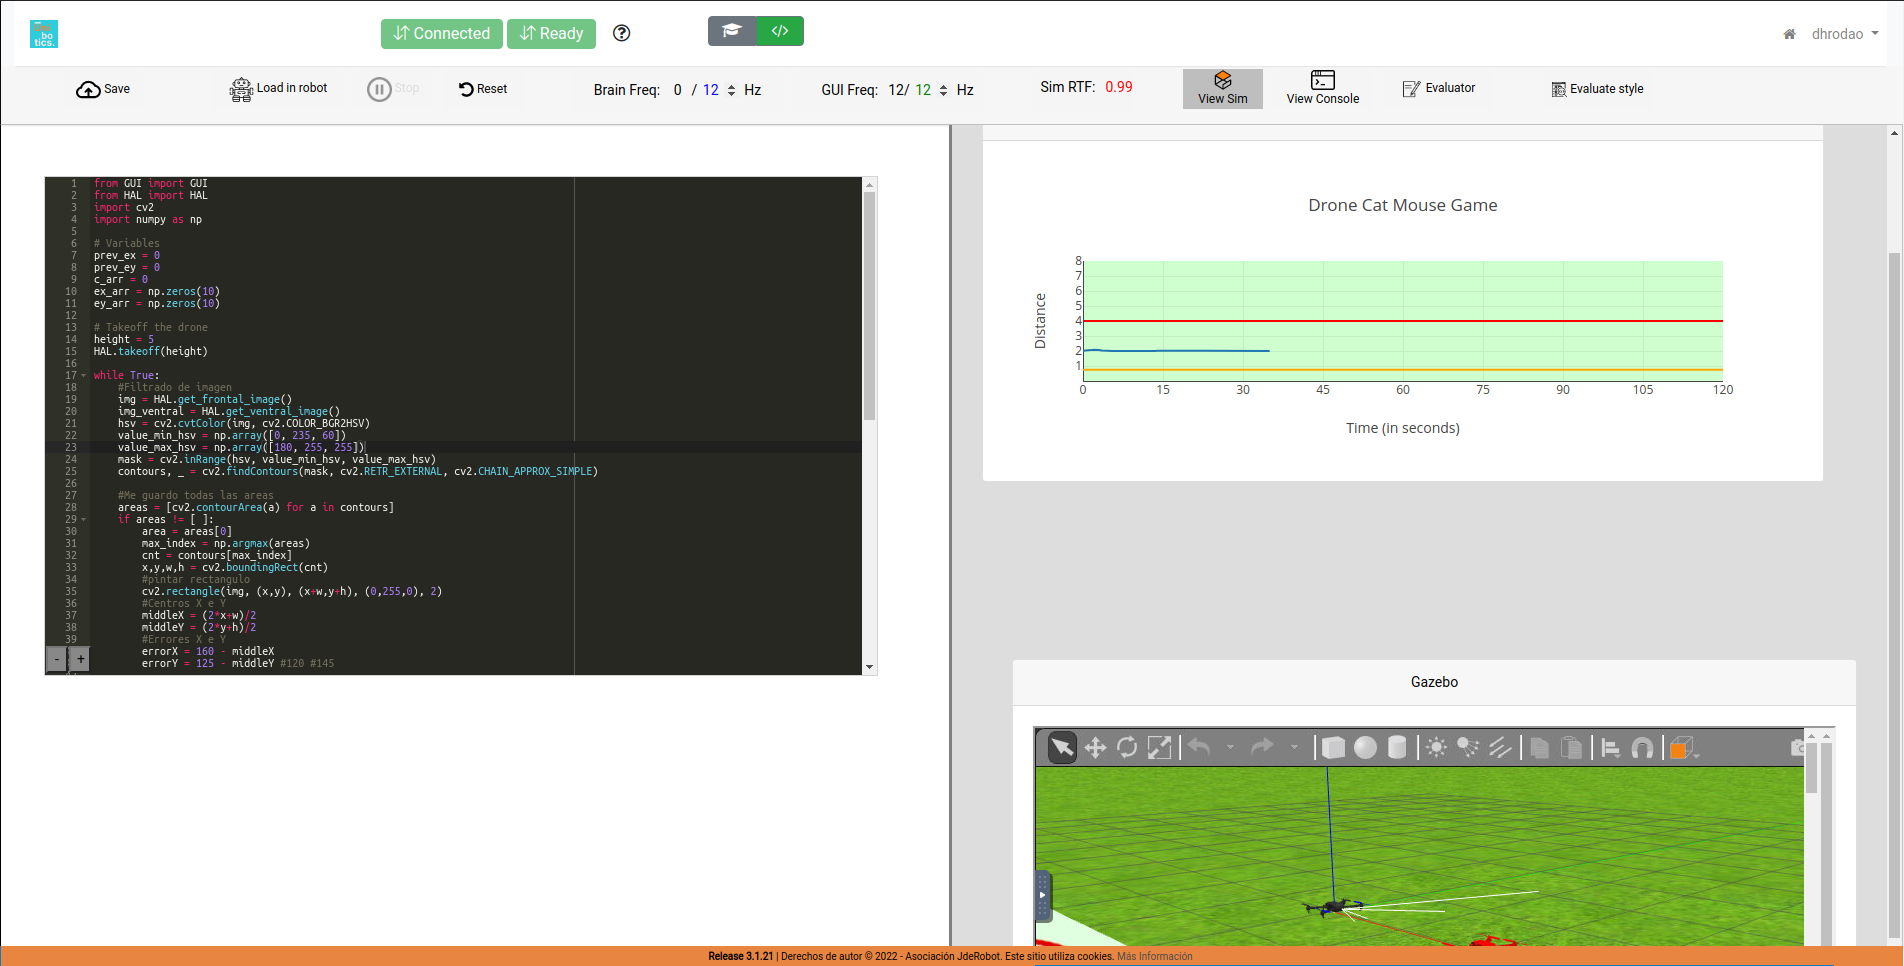
\includegraphics[width=\textwidth]{img/drone_cat_mouse.png}
    \caption{Plantilla Drone Cat Mouse.}
    \label{figura:keyhandler}
\end{figure}

Por otro lado, la plataforma Unibotics contaba con una versión del reto \emph{Drone Cat Mouse} con una arquitectura en la que, internamente, el \emph{ratón} era instanciado dentro del controlador del robot que se correspondía con el \emph{gato}, y éste se controlaba desde el propio objeto del \emph{gato}.

En la versión desarrollada para este trabajo se han introducido algunos cambios. En primer lugar, se han desacoplado los controladores para los robots, de manera que ahora cada uno es independiente del otro. Esto da lugar a la necesidad de tener dos \emph{WebSockets para cada robot}. Inicialmente se tenían únicamente dos \emph{WebSockets} para comunicarse con el \emph{gato}, y este, se encargaba de trasladar la información al \emph{ratón}. Ahora hay dos \emph{ws\_code} y \emph{ws\_gui} para el \emph{gato} y el \emph{ratón} respectivamente.

En la versión inicial del ejercicio, el código del ratón se encontraba almacenado dentro del \emph{RADI}. Actualmente esto se ha cambiado, de manera que el código del \emph{ratón} se pide al \emph{webserver} especificando el ejercicio y la dificultad seleccionada. De esta manera, en la versión actual del ejercicio, el ratón recibirá el código que debe ejecutar vía su \emph{WebSocket} de código, mientras que en la versión inicial, el ratón recibía una orden con la dificultad a ejecutar, y, finalmente, éste buscaba el código a ejecutar dentro del contenedor RADI. Este cambio se ha realizado con el fin de seguir el mismo paradigma que con los usuarios, el código fuente de los bots y ratones se recibe desde el \emph{webserver}. Una vez recibido el código, éste es enviado al \emph{ratón} por medio del \emph{WebSocket} correspondiente.

\subsection{Evaluador automático}
\label{drone_cat_mouse_evaluator}

En una versión inicial, la plataforma no disponía del \emph{Juego Drone Cat Mouse}, sino, del \emph{Reto Drone Cat Mouse}, es decir, este ejercicio inicialmente no incorporaba un evaluador automático que proporcionase un desafío para el usuario, por lo que se decidió incluir este evaluador para dar lugar al \emph{Juego Drone Cat Mouse}. 

Este evaluador automático consiste en una gráfica que muestra la distancia 3D medida entre el gato y el ratón en el tiempo. La gráfica se genera con una librería de \emph{JavaScript} llamada \emph{Plotly} \footnote{\url{https://plotly.com/javascript/}}, en la cual se muestra la distancia en el eje vertical y el tiempo en el eje horizontal.

\begin{figure}[H]
	\centering
    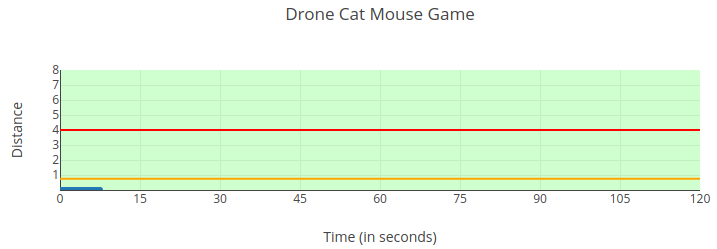
\includegraphics[width=16cm]{img/evaluator_drone_cat_mouse.png}
    \caption{Evaluador Drone Cat Mouse.}
    \label{figura:evaluator_drone}
\end{figure}

A continuación, se adjunta la parte principal del código fuente diseñado para la implementación de este evaluador automático.

\begin{lstlisting}[basicstyle=\ttfamily\scriptsize]
function startevaluate() {
    // reset score and dist
    score = 0.0;
    dist = 0.0;

    // submit code
    if (running == false) {
            start();
    }

    // stop existing plot if any
    var eval = undefined;
    clearInterval(eval);

    data = {
        data : [{ y: [dist_value] }],
        layout : {
            title : "Drone Cat Mouse Game",
            width : 800, 
            height : 300, 
            plot_bgcolor : "#cfffcf",
            xaxis : {
                range : [0, 240], 
                title : "Time (in seconds)", 
                tickvals : [0,30,60,90,120,150,180,210,240],
                ticktext : [0,15,30,45,60,75,90,105,120]
            }, 
            yaxis : {
                range : [0, 8], 
                title : "Distance", 
                tickvals : [1,2,3,4,5,6,7,8]
            },
            shapes:[
                // Puntuation Threshold Line 
                {
                    type:"line",
                    x0:0,
                    y0:4,
                    x1:240,
                    y1:4,
                    name:"Puntuation Threshold",
                    line:{
                        color:"red",
                        width: 2,
                    }
                },
                // Distance Warning Line (too close) 
                {
                    type:"line",
                    x0:0,
                    y0:0.75,
                    x1:240,
                    y1:0.75,
                    name:"Dangerous Distance",
                    line:{
                        color:"orange",
                        width: 2,
                    }
                }
            ]
        }
    };

    Plotly.newPlot("eval", data)
    var cnt = 0;

    eval = setInterval(function() {
        Plotly.extendTraces("eval", { y:[[dist_value]]}, [0]);
        cnt++;
        /*
        if (cnt >= 240) {
            clearInterval(eval);
            eval_button.disabled = false;
            eval_button.style.opacity = "1.0";
            eval_button.style.cursor = "default";
        }
        */
        // change background color of the plot to red when distance > 4
        if(dist_value > 4) {
            Plotly.relayout("eval", {plot_bgcolor: "#ffcccb"});
            relayout_plot = true;
        } else if (dist_value <= 4 && relayout_plot == true ) {
            if(dist_value >= 0.75){
                Plotly.relayout("eval", {plot_bgcolor: "#cfffcf"});
            }else{
                Plotly.relayout("eval", {plot_bgcolor: "#f4b786"});
            }
            relayout_plot = false;
        }

        // calculate and display score
        calculate_score();
    },500);
}
\end{lstlisting}

\subsection{Robots adversarios: modelo 3D y cerebros}

El modelo 3D empleado para el robot \emph{ratón} se corresponde con el mismo modelo que el del \emph{gato}. Adicionalmente, para diferenciarlos, el color del modelo del \emph{ratón} se establece al rojo. Siendo los colores de los modelos negro (\emph{gato}) y rojo (\emph{ratón})

Para este juego, han sido implementados tres códigos diferentes que se corresponden con los tres oponentes automáticos con sendas dificultades crecientes proporcionadas por la plataforma. Han sido cargados en el juego Gato-Ratón de los correspondientes perfiles creados para la gestión de los oponentes. La dificultad se corresponderá con el patrón de movimiento que realiza el dron \emph{ratón}, es decir, a mayor dificultad, el \emph{ratón} realizará un patrón de movimiento más complejo.

\begin{lstlisting}
def path1(t):
	"""
	Start and stop path
	"""
	if round(t / 2) % 2 == 0:
		vx = 3
	else:
		vx = 0

	vy = 0
	vz = 0
	az = 0

	return vx, vy, vz, az
	
# Takeoff the drone
height = 5
HAL.takeoff(height)

while True:
    # Enter iterative code!
    t = time.time()
    vx, vy, vz, yaw = path1(t)
    HAL.set_cmd_vel(vx, vy, vz, yaw)
\end{lstlisting}

El código anterior se corresponde con la dificultad más sencilla de los bots proporcionados para el ejercicio Gato-Ratón. En este código se puede apreciar cómo en cada una de las iteraciones, se está generando una velocidad aleatoria en el \emph{eje x} de la simulación. En esta dificultad, el \emph{ratón} únicamente se desplazará a lo largo del \emph{eje x} con distintas velocidades.

\subsection{Carga del código del cerebro del robot}
\label{drone_cat_mouse_code_load}

La versión del juego de la que se parte contenía únicamente un controlador para el robot en el que se cargaba el código del usuario (\emph{gato}), y éste era el encargado de dar las órdenes al otro robot (\emph{ratón}) para cargar el código, pararse, etc.

Puesto que los ejercicios asíncronos han sido pensados desde el punto de vista de tener dos robots bien diferenciados en el escenario, los controladores de los robots se han reimplementado. De manera que, el robot \emph{gato} tiene su propio controlador y ya no da órdenes al \emph{ratón}. Se ha desacoplado la dependencia entre ambos robots. Para llevar a cabo esto, ha sido necesario replicar el controlador del \emph{gato} para hacerlo funcionar también con el \emph{ratón}. Al hacer este desacoplamiento han aparecido dos \emph{WebSockets} adicionales, que se corresponden el robot \emph{ratón}. 

De esta manera, cada robot tendrá sus \emph{WebSockets} separados, y actuará independientemente del otro robot. Además, las cargas de código se harán para cada robot por medio de su \emph{WebSocket} de código.

La carga de código se realiza de manera similar al ejercicio anterior. Una vez realizada la comprobación de código y su carga, se habilita el botón \emph{Play}.

\subsubsection{Inicio del juego}
\label{drone_cat_mouse_inicio}

De igual manera que en el juego \emph{Follow Line}, primeramente hay que realizar la conexión con \emph{RADI}, que se encargará de lanzar el proceso del juego, y, una vez se haya establecido la conexión con los \emph{WebSockets}, se avisa al \emph{Front End} de manera que el usuario quede notificado. Posteriormente, puede elegirse la dificultad del ratón, cargar el código del usuario, mostrar \emph{Gazebo} y la consola,  y reanudar la simulación.

\subsection{Selección de dificultad}
\label{drone_cat_mouse_difficulty}

El selector de dificultad del \emph{ratón} al que se va a enfrentar el drone gato está situado en la mitad superior derecha de la interfaz del usuario junto a los botones de control del mismo. El usuario debe seleccionar primeramente la dificultad deseada mediante el desplegable situado en la mitad derecha de la pantalla. Y, a continuación, pulsar el botón \emph{Load in robot} para proceder a la carga de los códigos.

Para realizar la carga de códigos, primero se obtiene el código del editor de texto situado en la mitad izquierda de la plantilla y se envía por el \emph{WebSocket} empleado para comunicarse con el \emph{gato}. A continuación, mediante una peticón HTTP al \emph{WebServer}, se solicita el código del ratón (en función de la dificultad), y finalmente se envía por el \emph{WebSocket} definido para la comunicación  \emph{RADI}-\emph{Ratón}.

\begin{figure}[H]
	\centering
    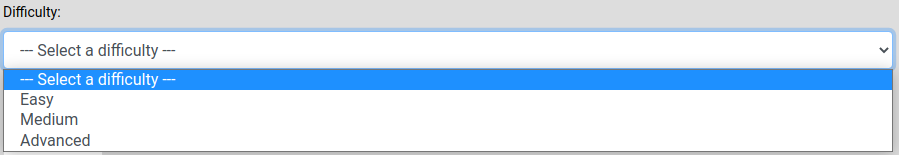
\includegraphics[width=\textwidth]{img/drone_cat_mouse_difficulty.png}
    \caption{Selector de dificultad Drone Cat Mouse.}
    \label{figura:evaluator_drone}
\end{figure}

\subsection{Validación experimental}
En este ejercicio el proceso para iniciar la conexión con RADI es similar al del juego Follow Line. 

\begin{figure}[H]
	\centering
    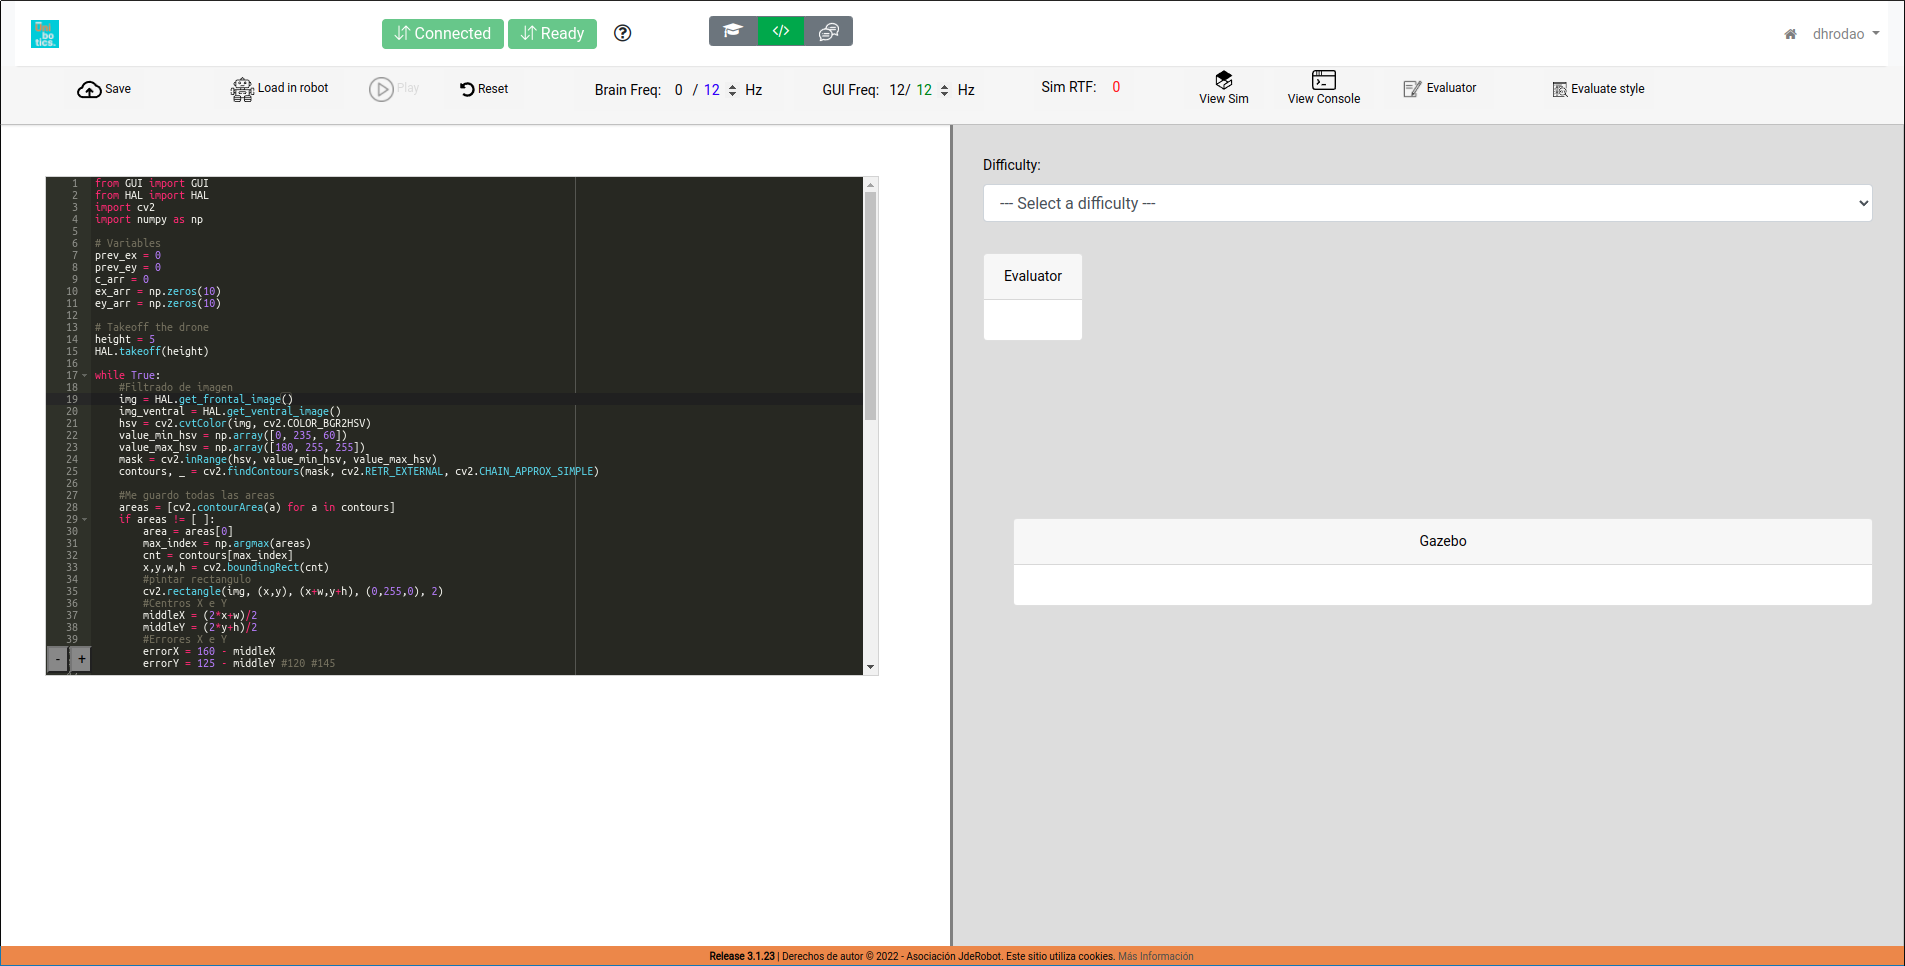
\includegraphics[width=\textwidth]{img/dcm_conectado.png}
    \caption{Drone Cat Mouse lanzado.}
    \label{figura:evaluator_drone}
\end{figure}

Una vez lanzado el ejercicio, el usuario debe proceder a la selección de la dificultad del dron ratón. A continuación, cargar el código en los robots. Y finalmente, abrir el visor Gazebo, el evaluador automático e iniciar la simulación pulsando el botón \emph{Play}.

\begin{figure}[H]
	\centering
    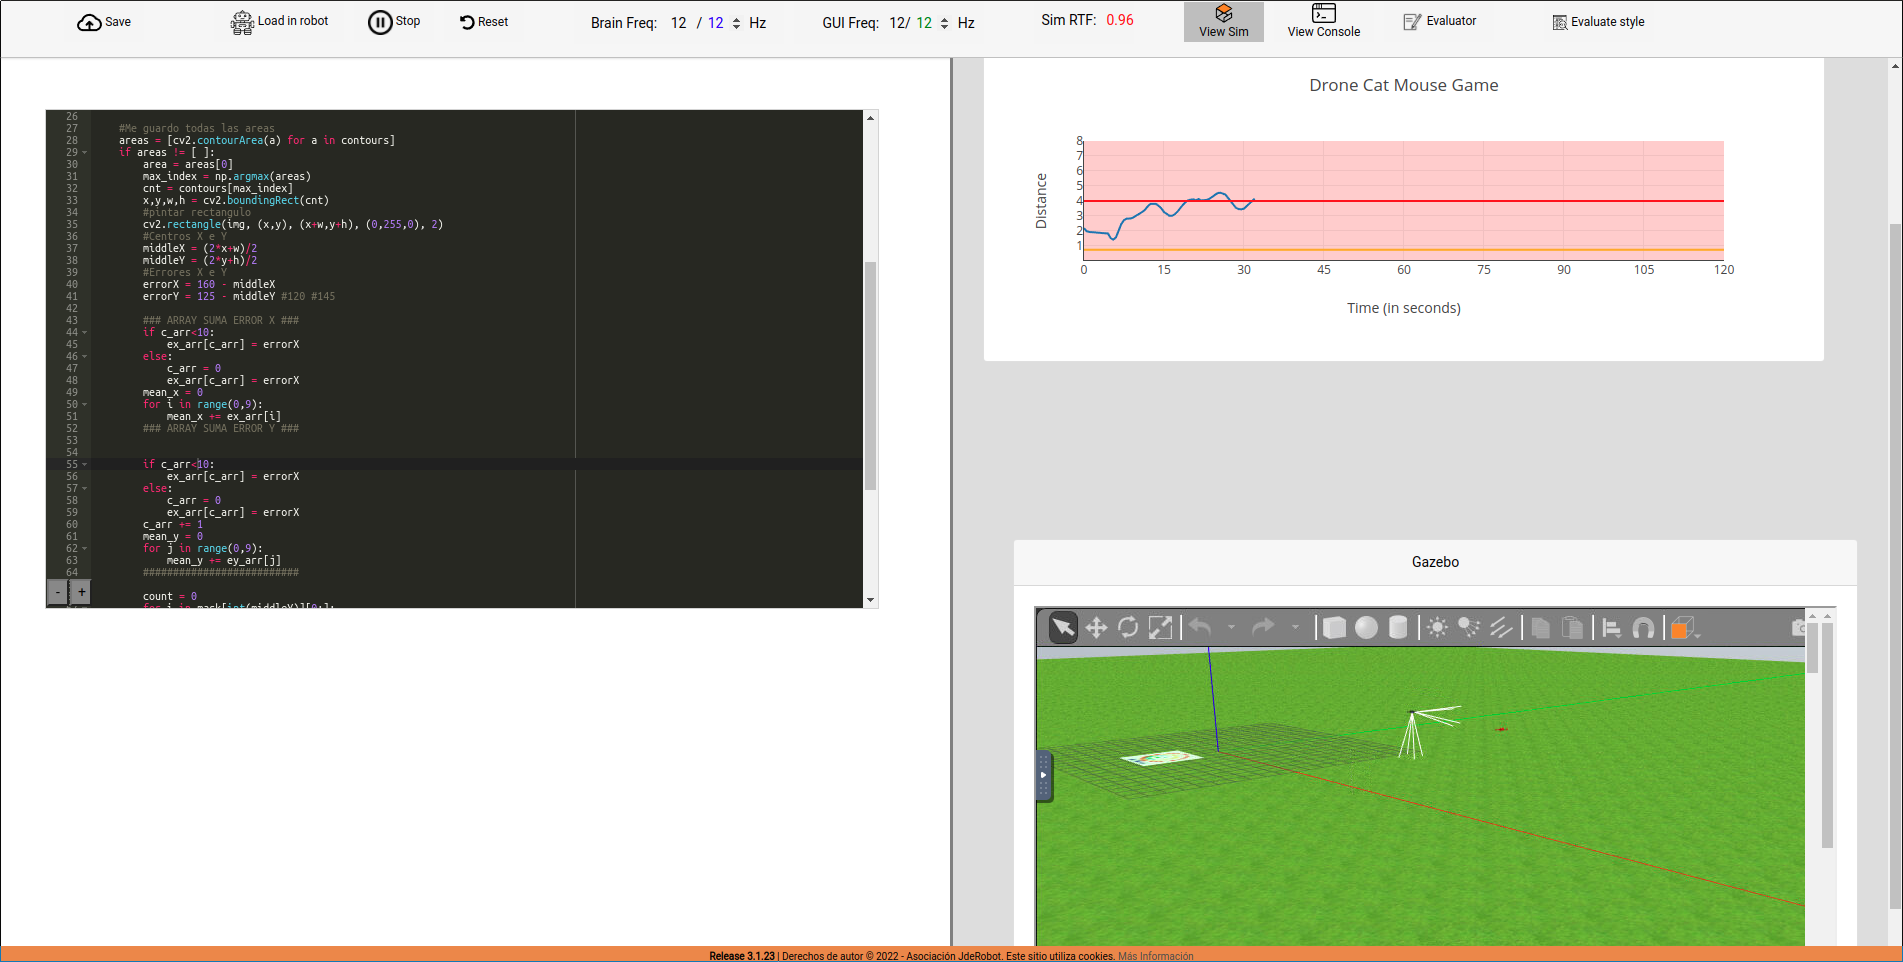
\includegraphics[width=\textwidth]{img/dcm_sim.png}
    \caption{Simulación y evaluador automático en Drone Cat Mouse.}
\end{figure}

Con el objetivo de una mejor comprensión del funcionamiento del ejercicio se ha elaborado un vídeo de manera que se tenga un ejemplo más ilustrativo. Está disponible en YouTube en el enlace \textbf{\url{https://www.youtube.com/watch?v=sXqZvsV5lzc}}.

%%%%%%%%%%%%%%%%%%%%%%%%%%%%%%%%%%%%%%%%%%%%%%%%%%%%%%%%%%%%%%%%%%%%%%%%%%%%%%%%
%%%%%%%%%%%%%%%%%%%%%%%%%%%%%%%%%%%%%%%%%%%%%%%%%%%%%%%%%%%%%%%%%%%%%%%%%%%%%%%%
% JUEGOS SÍNCRONOS %
%%%%%%%%%%%%%%%%%%%%%%%%%%%%%%%%%%%%%%%%%%%%%%%%%%%%%%%%%%%%%%%%%%%%%%%%%%%%%%%%

\cleardoublepage
\chapter{Juegos Compartidos Síncronos}

En \emph{Unibotics} se han desarrollado juegos asíncronos en los que se elige competir con uno de los advesarios automáticos, bots, proporcionados por la plataforma, sin embargo, en estos juegos no se explota la posibilidad de que dos usuarios reales puedan contrastar sus códigos con el de otros usuarios. Con el desarrollo los \emph{ejercicios síncronos} se han querido orientar los juegos hacia un modo más directo y dinámico, de manera que el usuario pueda conectarse con otros usuarios y competir entre ellos poniendo en ejecución sus mejores códigos.

En este capítulo se abordan todos los detalles de los \emph{juegos síncronos}. En una primera parte se detalla el diseño e implementación de las plantillas del usuario, para posteriormente, dirigirnos a los aspectos relacionados con las comunicaciones \emph{WebRTC} y el servidor web de \emph{Unibotics} como servidor de señalización entre los usuarios. En esta modalidad síncrona se ha desarrollado el juego del \emph{Sigue-Líneas}.

\section{Diseño de los juegos síncronos}
\label{sync_design}

Se trata de un juego síncrono en el que participan dos usuarios de manera simultánea en un ejercicio. A continuación, se hablará del rol de cada uno de los usuarios, el anfitrión y el invitado.

En función del rol, cada usuario tendrá una interfaz del ejercicio diferente, adaptada a sus funciones. El usuario anfitrión es el usuario que se encarga de la ejecución del ejercicio en su máquina local mediante el contenedor Docker (RADI), y se encarga de compartir el simulador Gazebo al usuario invitado vía \emph{WebSockets} mediante un flujo multimedia. 

La simulación también genera otros datos adicionales además de la visualización de Gazebo, estos son, los datos del evaluador automático y la vista de pájaro, que son compartidos via \emph{WebSockets} a través de un canal (\emph{DataChannel}) junto a los mensajes del chat. 

Con objeto de finalizar la ejecución del ejercicio, se ha desarrollado una funcionalidad con la que ambos usuarios pueden terminar a la conexión mediante un botón de finalización de conexión. Este botón hará que ambos navegadores vuelvan a cargar la página del ejercicio, quedando los dos usuarios listos para realizar otra conexión síncrona.

Con respecto a la transmisión de los datos (flujo multimedia, mensajes de chat, datos de la IU, botones Play/Reset pulsados por el invitado, botón reset pulsado por el anfitrión, finalización de la conexión por uno de los pares), las conexiones entre los dos pares se realizan sin intermediarios en el caso de que exista una conexión favorable (como una red local, en la que no intervienen NATs que dificulten la conexión entre los pares) entre ambos. En los casos en los que se dificulta la conexión, se emplea un servidor TURN que se encarga de retransmitir el tráfico que genera cada unos de los extremos y enviarlo hacia el par opuesto. A continuación se incluye una imagen (figura \ref{figure:disenio_juego_sincrono}) que ilustra el diseño del juego síncrono al completo:

\begin{figure}[H]
	\centering
    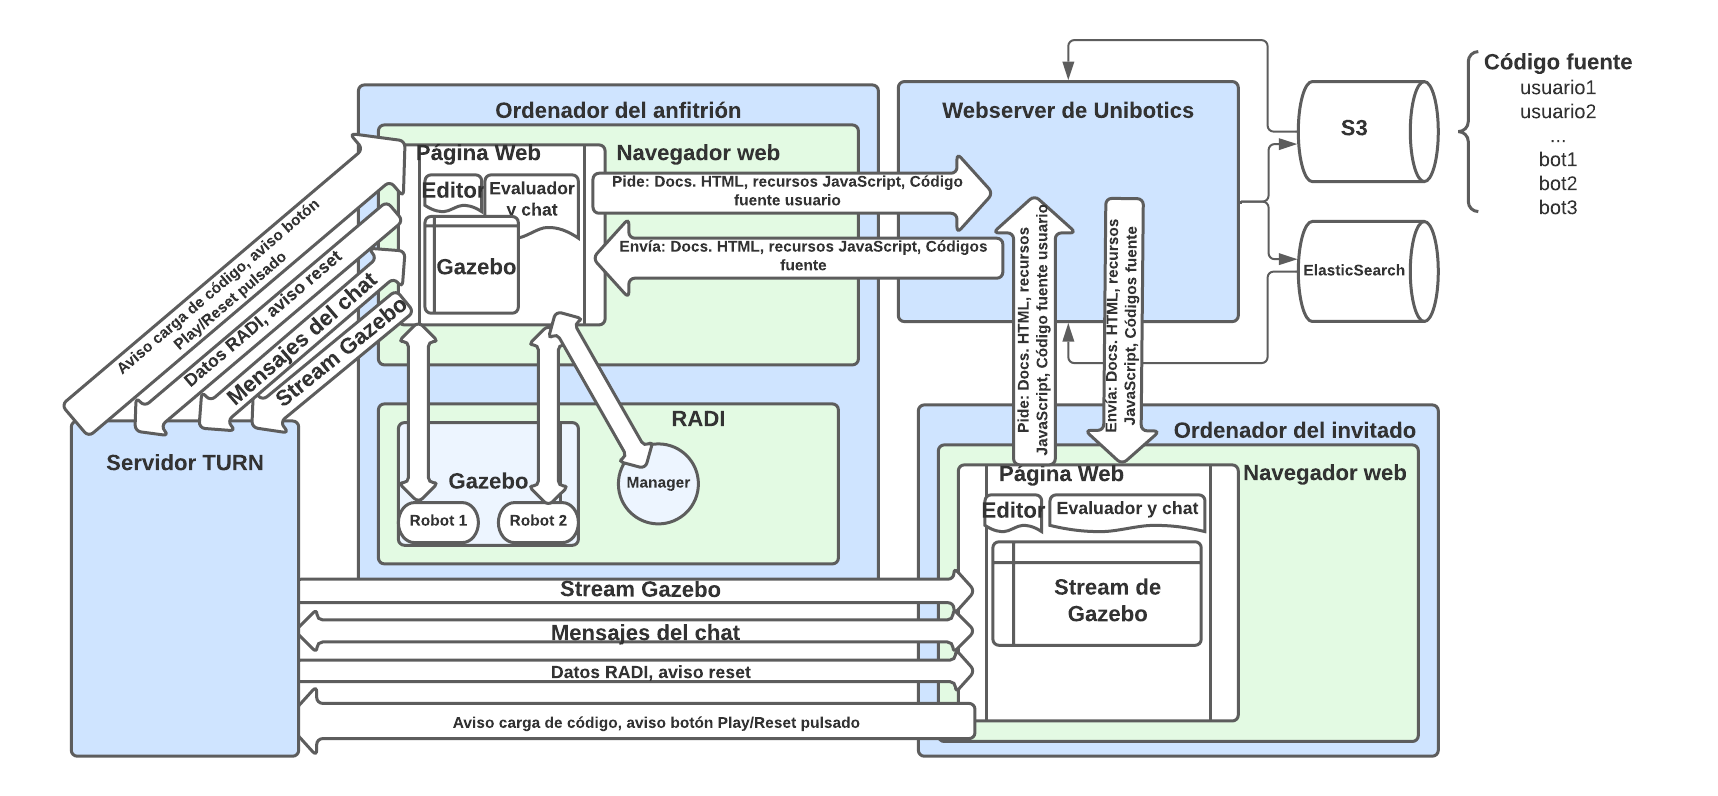
\includegraphics[width=18.5cm]{img/diagrama_sincrono.png}
    \caption{Diseño de juego síncrono.}
    \label{figure:disenio_juego_sincrono}
\end{figure}

\section{Follow Line Game Síncrono} 
\label{sec:follow_line_game_sync}

\subsection{Interfaz de usuario}

El juego \emph{Follow Line Síncrono} parte de la plantilla básica que comparten todos los ejercicios "monorrobot" de \emph{Unibotics}. A esta plantilla se le han añadido una serie de extras, como el chat de texto, la barra de búsqueda de usuarios oponentes y los botones de carga de código fuente, del anfitrión y del invitado. Adicionalmente, se ha añadido un botón para ocultar el editor de código con el fin del que el usuario tenga únicamente la vista del chat de texto.

Con respecto a la interfaz del usuario invitado, esta interfaz se autoajusta cuando el usuario acepta la invitación proveniente de un anfitrión. Este ajuste se realiza mediante el lenguaje \emph{JavaScript}, en el que se ha implementado código que se encarga de ocultar los elementos de la interfaz que no se quieren visualizar en el extremo del invitado.
%% AÑADIR CAPTURA DE LA PLANTILLA
\begin{figure}[H]
	\centering
    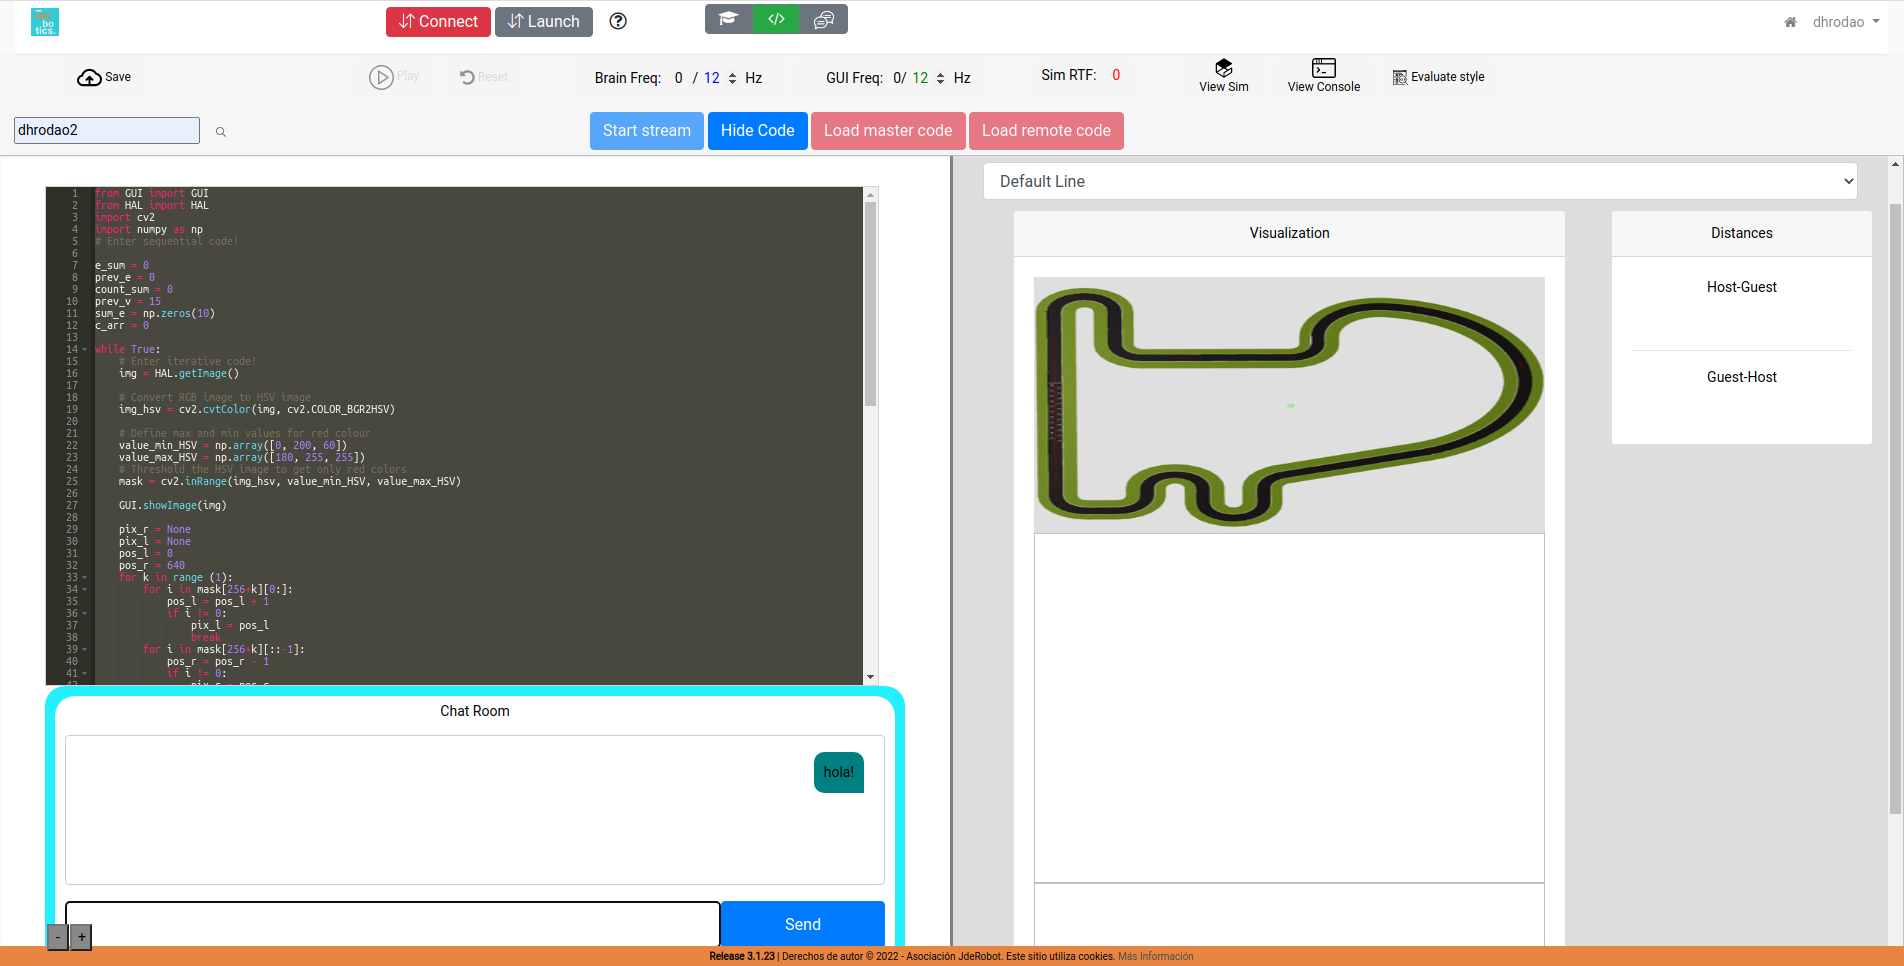
\includegraphics[width=15cm]{img/follow_line_game_sync.png}
    \caption{Plantilla del juego Follow Line en Unibotics.}
    \label{figura:diagrama_conexion_webrtc}
\end{figure}

\subsection{Sistema de salas de juego}

Para desarrollar este ejercicio, ha sido necesario implementar \emph{software} tanto del lado del cliente como del lado del servidor. Los usuarios participantes deben usar el servidor web de \emph{Unibotics} como servidor de señalización para el protocolo \emph{WebRTC}. Una vez ambos extremos se conocen entre sí, se inicia el tráfico \emph{WebRTC} entre ellos.

Una vez el usuario entra en el ejercicio, automáticamente el navegador se conecta a una ruta del servidor web por medio de \emph{WebSockets} generando una sala de juego. Esta ruta será el medio a través del cual se van a comunicar los dos extremos con el servidor de señalización.

Debido a la complejidad de las subredes, ha sido necesaria la incorporación de un servidor \emph{TURN} (\emph{Transversal Using Relay NAT}) que se encargue de hacer de retransmisor entre los dos extremos si no es posible establecer la conexión directa una vez se inicia la comunicación \emph{WebRTC}. En la mayoría de casos no es posible realizar una conexión \emph{WebRTC} directa entre los dos extremos (a menos que residan en una red local). Esto es debido a que \emph{WebRTC} no es capaz de atravesar un NAT (\emph{Network Address Translation}). Este servidor TURN se encarga de retransmitir el tráfico de la conexión WebRTC en caso de que falle la conexión directa entre ambos extremos. TURN se encarga de resolver estas incompatibilidades y permite que cualquier dispositivo pueda establecer una conexión WebRTC. Este servicio implica un mayor consumo de ancho de banda y un aumento de la latencia, pero en algunas ocasiones es la única solución eficaz para garantizar conexiones fructuosas entre cualquier dispositivo.
%% AÑADIR CAPTURA DE ARQUITECTURA

\subsection{Elección de oponente}
\label{sec:follow_line_game_sync_oponente_chat}

Para proporcionar al usuario la elección de un contrincante, se ha implementado una barra de búsqueda de usuarios que permite al anfitrión escribir el nombre del usuario que desea invitar.

Una vez el usuario realiza la selección del contrincante, una petición es enviada al servidor web por medio del \emph{WebSocket} de la sala de juego, y este la reenviará al usuario invitado en caso de que se encuentre en línea y dentro del mismo ejercicio. Por otra parte, en el caso de que el usuario al que se invita no esté disponible, ya sea porque no existe, o porque no se encuentra disponible dentro del mismo ejercicio, el servidor web responderá al navegador anfitrión con un mensaje de error, y se mostrará un cuadro de diálogo en la interfaz avisándole.

En el caso de que el invitado acepte la solicitud, el anfitrión comenzará con la negociación \emph{WebRTC}. 

\subsubsection{Barra de búsqueda}

Para realizar la conexión entre dos usuarios, el anfitrión debe escribir el login del usuario que quiere invitar en la barra de búsqueda de usuario, de manera que se pueda hacer la consulta al servidor web. Se ha desarrollado código \emph{JavaScript} que se encarga de esperar a que se inserte el nombre de usuario y se pulse el botón "\emph{Enter}", y además, que se encargue de enviar lo insertado al servidor web vía el \emph{WebSocket} establecido para la sala del juego.

Una vez el servidor recibe este mensaje por el \emph{WebSocket}, se encarga de extraer el nombre del usuario, y mediante el uso de un paquete instalado en el servidor \emph{Django}, llamado \emph{"Django-online-users"}, obtiene los usuarios que hay conectados actualmente, y comprueba si el usuario recibido se encuentra en línea y dentro del juego Follow Line esperando la invitación. En el caso en que la búsqueda no sea satisfactoria, se envía un mensaje al usuario anfitrión indicando la imposibilidad de realizar la invitación. Si la búsqueda se realiza con éxito, se envía la invitación a dicho usuario por \emph{WebSocket}.

En el lado del usuario receptor, el navegador recibirá la petición y la mostrará al usuario por medio de un menú de diálogo que le da la posibilidad de aceptar o rechazar la invitación.
%% AÑADIR CAPTURA DE LA INVITACIÓN
\begin{figure}[H]
	\centering
    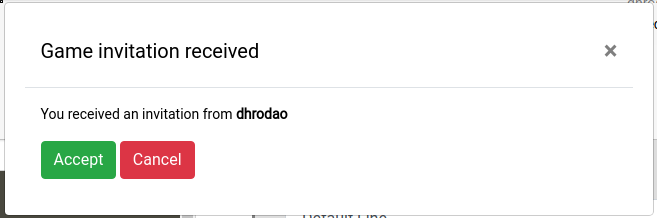
\includegraphics[width=10cm]{img/invitation.png}
    \caption{Diálogo de invitación recibida.}
    \label{figura:diagrama_conexion_webrtc}
\end{figure}


Una vez aceptada, se iniciará la conexión \emph{WebRTC}. Y el usuario anfitrión será el encargado de iniciar la simulación y compartir la retransmisión.

\subsubsection{Sección de chat}

Como se ha mencionado antes, la plantilla del juego contiene un chat que permite la comunicación vía texto entre ambos usuarios. Este chat se ha implementando usando una conexión \emph{WebRTC} y \emph{DataChannels} entre los navegadores, de manera que se reduce la carga de tráfico que atraviesa el servidor web, pues estos mensajes son enviados por medio del canal de datos \emph{peer-to-peer}.

Este sistema se ha desarrollado en el lado del cliente, mediante un \emph{script} en \emph{JavaScript} que contiene toda la configuración para realizar la creación de los \emph{DataChannels}. Además, se ha implementado una función de \emph{callback} (\emph{onDataChannelMessage}) que es ejecutada cuando se recibe un mensaje por el \emph{DataChannel} y que se encarga de añadir el mensaje al chat.

\subsubsection{Transmisión de datos entre plantillas}

El \emph{DataChannel} es aprovechado para el paso de más información además de para el envío de los mensajes del chat. Una vez el anfitrión conecta el \emph{RADI} en su máquina local, por este \emph{DataChannel} son enviados todos los datos recibidos desde el contenedor docker RADI para que el navegador del usuario invitado también los muestre en su interfaz gráfica. Es decir, la vista de pájaro, y el evaluador automático. Adicionalmente, cuando el usuario invitado presione el botón \emph{Play} o el botón de carga de su código, estas órdenes serán enviadas al anfitrión por medio del canal de datos, que será quien las complete.

\begin{figure}[H]
	\centering
    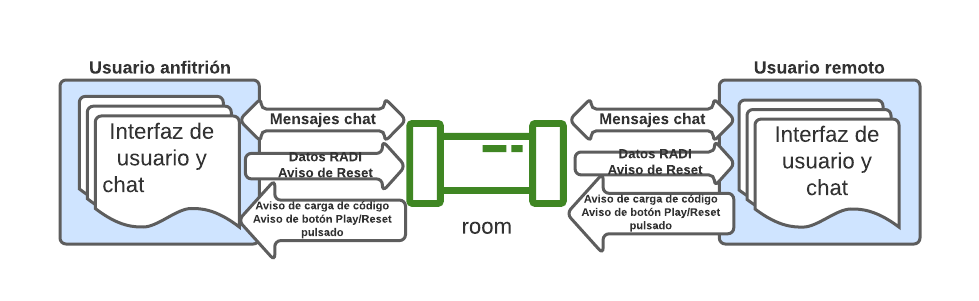
\includegraphics[width=15cm]{img/transmision_datos.png}
    \caption{Diagrama de transmisión de datos entre plantillas.}
    \label{figura:diagrama_conexion_webrtc}
\end{figure}

\subsection{Transmisión de vídeo y datos vía WebRTC}

Una vez elegido el oponente y aceptada la invitación, ha sido necesario el desarrollo de las fases descritas en la sección \ref{subsec:establecimiento_conexion} de manera que se pueda negociar una conexión entre los dos extremos.

Dependiendo del extremo de la conexión que sea el usuario (\emph{caller} o \emph{callee}), necesita realizar unos pasos u otros, por lo que para cada extremo se necesita un código diferente, este código se ha recogido en un fichero llamado \emph{"rtc\_stream.js"}.

En primer lugar, se ha creado una función llamada \emph{startLocalStream}, que se encarga de realizar la conexión desde el lado del anfitrión. Estos son los primeros 6 pasos detallados en la sección \ref{subsec:establecimiento_conexion}.

Desde el lado del usuario invitado, se ejecutará una función llamada \emph{startRemoteStream}, que una vez se reciba desde el servidor web la oferta enviada por el anfitrión mediante \emph{WebSockets}, se encargará de realizar los pasos 7-11 descritos en la sección \ref{subsec:establecimiento_conexion}.

Finalmente, en el lado del anfitrión se recibirá desde el servidor web la respuesta del otro extremo. Una vez recibida la respuesta, se almacena el \emph{SDP} \footnote{\url{https://es.wikipedia.org/wiki/Session_Description_Protocol}} (\emph{Session Decription Protocol}) del extremo remoto. Una vez establecida la descripción del otro extremo, ambos pares tienen la identificación del otro, por lo que puede iniciarse una comunicación \emph{WebRTC}.

Para realizar el envío de sus candidatos, cada par debe enviarlos al servidor de señalización (haciendo uso de la función \emph{onIceCandidate}, como respuesta al \emph{callback} \emph{icecandidate}) para que este los reenvíe al otro par. En primer lugar, en el extremo remoto se reciben los candidatos. Este debe almacenar los candidatos (la función \emph{remotePeer.setRemoteDescription(offer)} establece la descripción de los candidatos remotos recibidos por parámetro en la función \emph{startRemoteStream}), y responder con su oferta. Finalmente, en el extremo local, se reciben los candidatos del par remoto y se establece el SDP del usuario invitado. Una vez realizado este paso, ambos extremos tienen el SDP del extremo remoto, por lo que pueden iniciar la elección del mejor candidato ICE, y, posteriormente el establecimiento de la conexión \emph{WebRTC} entre ellos dos.

Gracias a este sistema, se permite que los usuarios tengan una conexión directa entre ellos, y únicamente un usuario ejecute el simulador, puesto que el elemento \emph{HTML} que contiene el vídeo del simulador es retransmitido al otro extremo haciendo uso de la conexión entre pares.

Para soportar el intercambio de cantidatos ICE entre los extremos, se ha implementado en el servidor web \emph{Django} un sistema de señalización entre usuarios basado en salas usando \emph{Django-channels} \footnote{\url{https://channels.readthedocs.io/en/stable/}}. Ha sido necesario implementar un objeto (\emph{StreamConsumer}) en el fichero \emph{consumers.py} que contiene la funcionalidad necesaria para el soporte de grupos, y el reenvío de mensajes al extremo remoto.

De igual manera, en el lado del \emph{DataChannel}, la implementación del establecimiento de los candidatos ICE es similar al sistema implementado para la tranmisión de vídeo, únicamente ha sido necesario cambiar la parte del \emph{streaming} por una parte con el establecimiento de un canal de datos, por el que viaja todo lo relativo a la IU y a los mensajes del chat entre los dos pares, y en conexiones complicadas atravesando un servidor TURN. En el lado del servidor, también ha sido necesario implementar un consumidor específico para la sala en el fichero "\emph{consumers.py}".

Este consumidor se encuentra en el lado del servidor web, y se encarga de establecer en una sala a cada usuario que entra en el ejercicio. Estas salas se crean con el objetivo de poder comunicar ambos extremos una vez se emparejan en una misma partida. Cuando el anfitrión invita a otro usuario, y este acepta la invitación, el consumidor procede a mover de sala al usuario invitado, colocándolo en la sala del anfitrión. Esto facilita en gran medida la señalización al servidor web, pues cuando este recibe un mensaje de un extremo, únicamente tiene que reenviarlo hacia el otro extremo.

Además, en ambos casos, en el lado del navegador ha sido necesaria la implementación de código para la gestión de los mensajes ente sockets, tanto para el \emph{WebSocket} de vídeo, como para el de datos. Este sistema se encarga de ejecutar la distintas fases del establecimiento de candidatos, como iniciar la conexión, añadir la descripción SDP remota una vez recibida, y señalizar al extremo remoto. Esta lógica se agrupa en dos ficheros, \emph{"ws\_stream.js"} para el vídeo y \emph{"ws\_room.js"} para el canal de datos.

\begin{figure}[H]
	\centering
    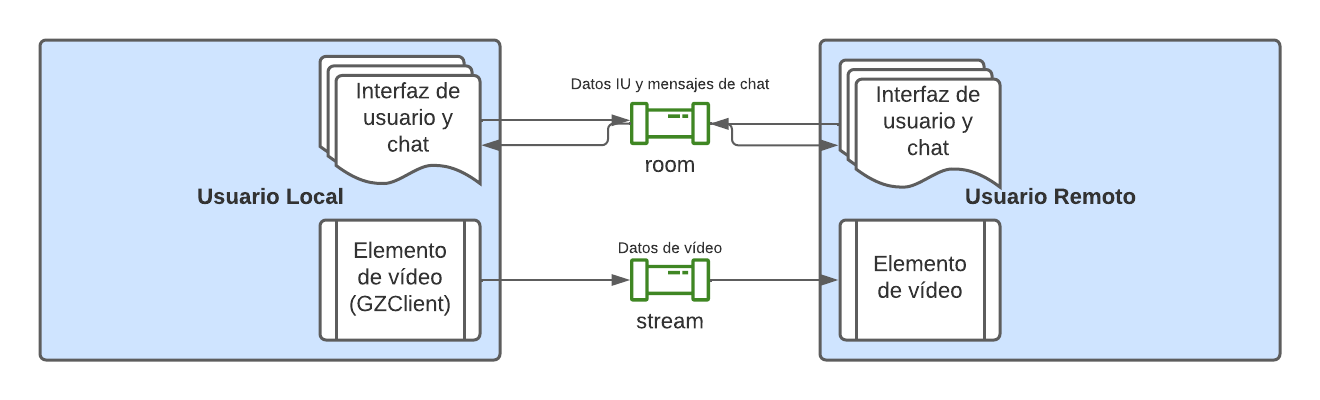
\includegraphics[width=16cm]{img/diagrama_conexion_webrtc.png}
    \caption{Diagrama de conexión WebRTC establecida con una conexión multimedia y un \emph{DataChannel}.}
    \label{figura:diagrama_conexion_webrtc}
\end{figure}

\subsection{Servidor TURN}

En los casos en los que la conexión entre los pares no es posible porque la topología de la red no lo permite, se emplea un servidor de retransmisión TURN. El cometido de este servidor es retransmitir el tráfico de un par al otro y viceversa.

Para el despliegue de este servidor, se ha empleado una herramienta de código abierto ya existente, llamada \emph{Coturn} \footnote{\url{https://github.com/coturn/coturn}}. Los desarrolladores de esta herramienta proveen una imagen Docker para desplegar el servidor de una manera sencilla.

Para desplegar este servidor se ha descargado la imagen Docker de \emph{Coturn} en una máquina de \emph{testing} de la universidad. A continuación, se ha utilizado el siguiente comando para el despliegue de contenedor: 

\begin{lstlisting}[basicstyle=\ttfamily\scriptsize]
sudo docker run -d --network=host coturn/coturn -n --log-file=stdout --listening-port=puerto --listening-ip=ip_maquina --relay-ip=ip_maquina --user=usuario:contrasenia --lt-cred-mech --verbose --realm=dominio_web
\end{lstlisting}

Mediante este comando se establece la IP del servidor, el puerto, las credenciales de acceso y el dominio (realm) para el que está sirviendo este servidor.

\subsection{Carga flexible de código}

Para proporcionar la libertad de la carga (es decir, que cada usuario pueda cargar su código cuando desee) del código fuente de uno y otro participante en sendos robots en el simulador, se ha desarrollado un módulo \emph{software} en \emph{JavaScript} que se encarga de soportar la carga flexible del código.

De esta manera, el código fuente de cada usuario debe cargarse en su robot respectivo antes de iniciar la simulación compartida. Con respecto al usuario invitado, se ha desarrollado un sistema que se encarga de avisar al usuario \emph{anfitrión} de que quiere cargar su código, mediante el \emph{DataChannel} establecido entre ambos. Una vez el \emph{anfitrión} recibe este mensaje, se encarga de pedir el código al \emph{WebServer} de \emph{Unibotics} y cargarlo en el coche correspondiente. En el lado de la carga de código del \emph{anfitrión}, simplemente, al pulsar el botón de carga de código, se pedirá el código al servidor web y se cargará en el robot correspondiente de modo similar a como se explicó en el capítulo anterior.

Una vez se carga un código, el botón de carga correspondiente se colorea de verde, de manera que para el usuario es más intuitivo a la hora de comprobar la situación de su código fuente.

Ambos navegadores sincronizan sus interfaces gráficas por medio del canal de datos establecido entre los navegadores enviando mensajes de control, que una vez son interpretados se aplican los cambios a la IU.

\subsection{Ejecución compartida}

Una vez se ha establecido la conexión \emph{WebRTC} entre los usuarios, y se ha cargado el código fuente en los robots, es necesario mostrar el estado de carga de los códigos y proporcionar una serie de controles de la ejecución de la simulación a los usuarios.

\subsubsection{Botones de control de la ejecución}

Existen varios elementos en la interfaz gráfica que son comunes a ambos usuarios. Estos son:

\begin{itemize}
\item \textbf{Botón \emph{Play}:} ambos usuarios tendrán la posibilidad de iniciar la ejecución del ejercicio una vez se han cargado los códigos en los robots.

\item \textbf{Botón \emph{Reset}:} botón que permite a ambos extremos realizar un reseteo del escenario compartido.
\end{itemize}

%% AÑADIR IMAGEN DE LOS BOTONES
  \begin{figure}[H]
  	\centering
    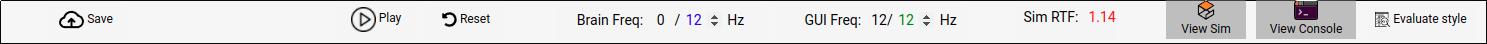
\includegraphics[width=10cm]{img/host_sync_control_bar.png}
    \caption{Barra de control del usuario anfitrión.}
    \label{figura:host_sync_control_bar}
  \end{figure}
  \begin{figure}[H]
  	\centering
    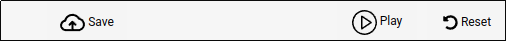
\includegraphics[width=10cm]{img/guest_sync_control_bar.png}
    \caption{Barra de control del usuario invitado.}
    \label{figura:guest_sync_control_bar}
  \end{figure}

Una vez cargados ambos códigos, se habilitará el botón \emph{Play} en ambos extremos. Desde el lado del usuario \emph{invitado}, se ha elaborado un sistema que se encarga de enviar las órdenes al usuario \emph{anfitrión} cuando algún botón es pulsado. Una vez el anfitrión recibe una órden, este se encarga de procesarla y ejecutar las órdenes. De esta manera, ambos usuarios pueden controlar de manera individual la ejecución de la simulación compartida.

\subsubsection{Botones de carga de código}

Para que los usuarios puedan conocer el estado de carga de sus códigos, se ha implementado un sistema que guarda el estado de carga y realiza una serie de ajustes visuales. Los indicadores de carga son los siguientes:

\begin{itemize}
\item \textbf{Botón de carga de código del anfitrión:} se encuentra únicamente en la plantilla del usuario anfitrión, este elemento es un botón que inicialmente tiene un color rojo, mostrando un estado que representa que no hay ningún código cargado. Una vez se carga el código, este botón cambia a un color verde.
\item \textbf{Botón de carga de código del invitado:} se encuentra ambas interfaces, este elemento es un botón que inicialmente tiene un color rojo, mostrando un estado que representa que no hay ningún código cargado. Una vez se carga el código, este botón cambia a un color verde en ambos extremos. Este botón no puede ser pulsado en el lado del anfitrión.
\end{itemize}

El establecimiento de los estados se realiza mediante mensajes vía \emph{WebSockets} entre ambos usuarios. En la plantilla del \emph{anfitrión} es donde se almacenan todas las variables relativas al estado de los códigos, el extremo \emph{invitado} únicamente recibe órdenes vía \emph{WebSockets} para actualizar su interfaz gráfica.

%% AÑADIR IMAGEN DE LOS BOTONES EN EL HOST Y EL GUEST
\begin{figure}[H]
  \centering
  \begin{minipage}[b]{0.3\textwidth}
  	\centering
    
\includegraphics[width=\textwidth]{img/host_code_buttons.png}
    \caption{Botones de control de código del anfitrión.}
    \label{figura:robot_davinci}
  \end{minipage}
  \hfill
  \begin{minipage}[b]{0.3\textwidth}
  	\centering
    
\includegraphics[width=\textwidth]{img/guest_code_buttons.png}
    \caption{Botones de control de código del invitado.}
    \label{figura:robot_atrias}
  \end{minipage}
\end{figure}


\subsection{Validación experimental}
La ejecución del ejercicio síncrono es similar a la de los ejercicios asíncronos. Para iniciar la conexión entre dos usuarios, uno de ellos ha de invitar al otro extremo. En el momento en que el extremo invitado acepta la invitación, se configura su interfaz y se establece la conexión WebRTC de datos entre ambos extremos. 

A continuación, el usuario anfitrión ha de lanzar la simulación pulsando el botón \emph{Launch} situado en la esquina superior izquierda de la pantalla, de manera que el RADI quede completamente preparado para la ejecución del ejercicio. Una vez se ha lanzado la simulación, el usuario anfitrión debe abrir el simulador Gazebo mediante el botón situado en la barra de control del ejercicio, de esta manera se habilitará el botón para iniciar el flujo de vídeo (botón \emph{Start stream}). 

Una vez pulsado este botón, se inicia la conexión WebRTC correspondiente con el flujo de vídeo (conexión llamada \emph{stream} en la Figura \ref{figura:diagrama_conexion_webrtc}). El resultado de una conexión fructuosa habilitará un elemento de vídeo en la plantilla del usuario invitado, donde será mostrada la ventana del simulador \emph{Gazebo} que está siendo ejecutado en la máquina del anfitrión.

  \begin{figure}[H]
  	\centering
    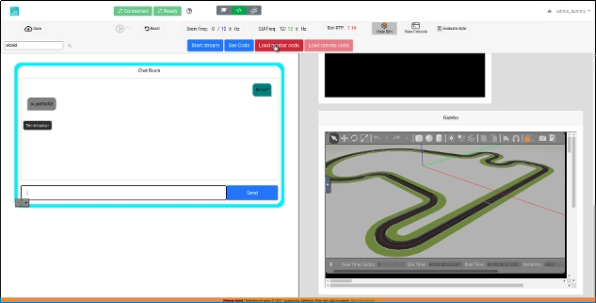
\includegraphics[width=\textwidth]{img/host_gazebo.png}
    \caption{Follow Line Game en usuario anfitrión.}
  \end{figure}
  \begin{figure}[H]
  	\centering
    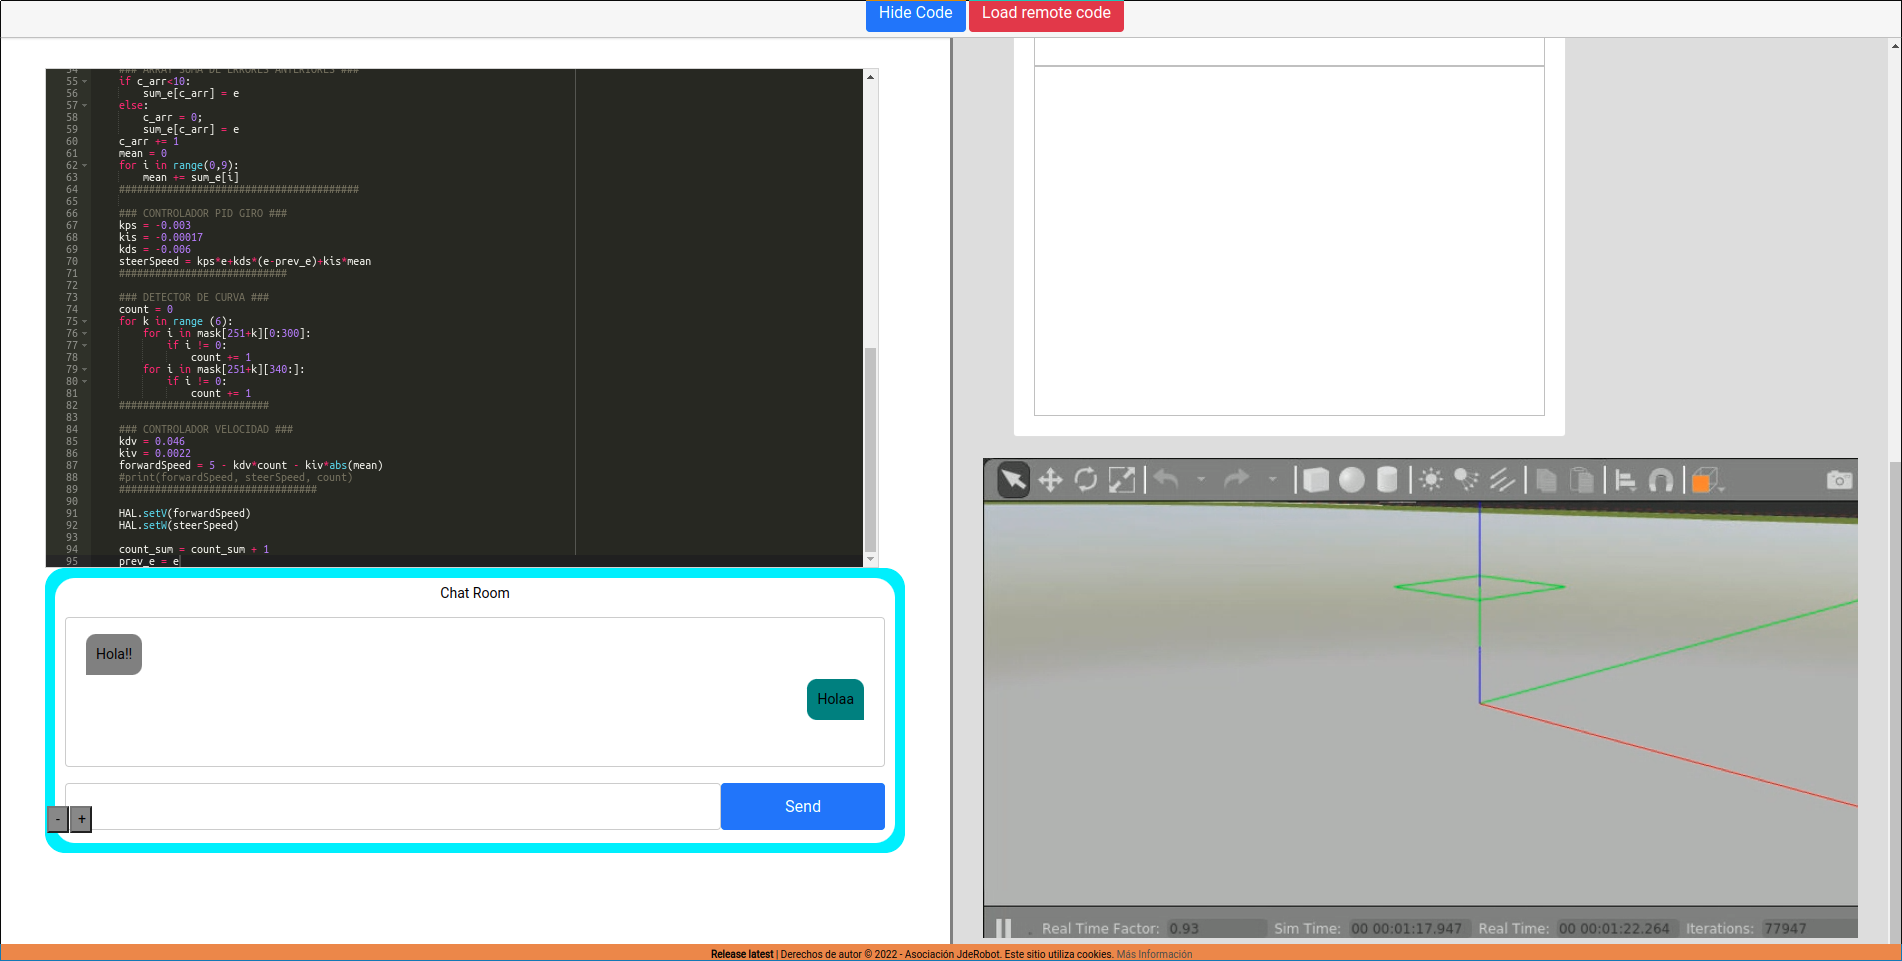
\includegraphics[width=\textwidth]{img/inv_gazebo.png}
    \caption{Follow Line Game en usuario invitado.}
  \end{figure}

Finalmente, uno de los dos usuarios podrá iniciar la simulación, mediante el botón \emph{Play} situado en su barra de control del ejercicio.

Con el objetivo de una mejor comprensión del funcionamiento del ejercicio se ha elaborado un vídeo ilustrativo que está disponible en YouTube (\textbf{\url{https://youtu.be/TC1fUieU1wI}}).

%%%%%%%%%%%%%%%%%%%%%%%%%%%%%%%%%%%%%%%%%%%%%%%%%%%%%%%%%%%%%%%%%%%%%%%%%%%%%%%%
%%%%%%%%%%%%%%%%%%%%%%%%%%%%%%%%%%%%%%%%%%%%%%%%%%%%%%%%%%%%%%%%%%%%%%%%%%%%%%%%
% EXPERIMENTOS Y VALIDACIÓN %
%%%%%%%%%%%%%%%%%%%%%%%%%%%%%%%%%%%%%%%%%%%%%%%%%%%%%%%%%%%%%%%%%%%%%%%%%%%%%%%%

%\cleardoublepage
%\chapter{Experimentos y validación}

%Este capítulo se introdujo como requisito en 2019. 
%Describe los experimentos y casos de test que tuviste que implementar para validar tus resultados. 
%Incluye también los resultados de validación que permiten afirmar que tus resultados son correctos. 


%%%%%%%%%%%%%%%%%%%%%%%%%%%%%%%%%%%%%%%%%%%%%%%%%%%%%%%%%%%%%%%%%%%%%%%%%%%%%%%%
%%%%%%%%%%%%%%%%%%%%%%%%%%%%%%%%%%%%%%%%%%%%%%%%%%%%%%%%%%%%%%%%%%%%%%%%%%%%%%%%
% RESULTADOS %
%%%%%%%%%%%%%%%%%%%%%%%%%%%%%%%%%%%%%%%%%%%%%%%%%%%%%%%%%%%%%%%%%%%%%%%%%%%%%%%%

%\cleardoublepage
%\chapter{Resultados}

%En este capítulo se incluyen los resultados de tu trabajo fin de grado.

%Si es una herramienta de análisis lo que has realizado, aquí puedes poner ejemplos de haberla utilizado para que se vea su utilidad.


%%%%%%%%%%%%%%%%%%%%%%%%%%%%%%%%%%%%%%%%%%%%%%%%%%%%%%%%%%%%%%%%%%%%%%%%%%%%%%%%
%%%%%%%%%%%%%%%%%%%%%%%%%%%%%%%%%%%%%%%%%%%%%%%%%%%%%%%%%%%%%%%%%%%%%%%%%%%%%%%%
% CONCLUSIONES %
%%%%%%%%%%%%%%%%%%%%%%%%%%%%%%%%%%%%%%%%%%%%%%%%%%%%%%%%%%%%%%%%%%%%%%%%%%%%%%%%

\cleardoublepage
\chapter{Conclusiones}
\label{chap:conclusiones}


\section{Conclusiones finales}
\label{sec:consecucion-objetivos}

El objetivo propuesto para este Trabajo de Fin de Grado era la gamificación de la plataforma de \emph{Unibotics} mediante la incorporación de una serie de juegos competitivos donde se involucran dos robots en el escenario cada uno con su propio cerebro. Este objetivo general se ha subdividido en dos subobjetivos bien diferenciados: los \emph{ejercicios asíncronos} y los \emph{ejercicios síncronos}.

El primer subobjetivo, ha sido alcanzado satisfactoriamente. En el lado del navegador se han desarrollado plantillas web para los ejercicios, evaluadores automáticos y manejadores para los selectores de dificultad. Y para el registro de las teclas de dirección del modo de teleoperación y el selector de circuito proporcionados en el juego Follow Line asíncrono. Además, también ha sido necesario implementar código del lado del servidor. Se han añadido una serie de usuarios con el prefijo \emph{botX} que contienen el código fuente de los cerebros de distintos niveles de dificultad. Adicionalmente, se ha creado un nuevo flujo en el servidor web que se encarga de devolver el código fuente de los respectivos bots en función de la dificultad seleccionada y el juego en que se encuentra el usuario. Finalmente, para el ejercicio Follow Line se ha diseñado, y programado el código que permite lanzar el ejercicio con el escenario Gazebo seleccionado en el selector de circuitos dentro de un conjunto de mundos posibles.

Dentro del primer subobetivo, se incluye también el juego del \emph{Gato-Ratón} con drones, alcanzado también de manera satisfactoria. Para el diseño de este juego, también ha sido necesario el diseño y la programación de plantillas web para el ejercicio. También, al igual que en el juego de \emph{Follow Line}, se hace uso de los bots, a los que se les añade el código para las distintas dificultades de este juego. Dentro del RADI, ha sido necesario remodelar este ejercicio, con el objetivo de desvincular el cerebro del \emph{ratón} del controlador del \emph{gato}: Es decir, se han creado dos controladores diferentes, uno para el \emph{ratón} y otro para el \emph{gato}. Cada uno se encarga de comunicarse con su correspondiente dron, para cargar el cerebro. Como fruto de esta modificación en el RADI, ha sido necesaria la creación de dos \emph{WebSockets} más en el lado del navegador, que se encargan de comunicarse con el nuevo controlador para el \emph{ratón}.

El segundo subobjetivo, el \emph{juego síncrono}, ha sido alcanzado de manera exitosa. Gracias a la tecnología WebRTC ha sido posible realizar competiciones síncronas entre usuarios. Para lograr este objetivo, en el lado del navegador ha sido necesaria la implementación de la plantilla web con sus respectivos manejadores. Adicionalmente, ha sido necesario elaborar una serie de scripts que se encargan de establecer las conexiones WebRTC entre los navegadores incluyendo una serie de escenarios de conectividad sencilla, con ambos participantes en la misma subred, como escenarios de conectividad complicada. Para estos últimos se ha preparato un servidor TURN que se encarga de resolver los problemas que generan las NAT. En el lado del servidor, se ha requerido la implementación de un sistema de comprobación de invitaciones y un sistema de salas de juego empleando \emph{Django-Channels} y \emph{Django-online-users}. Además, también ha sido necesario implementar un sistema de señalización en el servidor web que se encarga de permitir la negociación de la conexión WebRTC por parte de los dos extremos.

%\section{Aplicación de lo aprendido}
%\label{sec:aplicacion}


\section{Competencias adquiridas}
\label{sec:lecciones_aprendidas}

En este Trabajo de Fin de Grado se han ampliado y adquirido conocimientos de una serie de tecnologías que se recogen a continuación: \emph{HTML}, \emph{CSS}, \emph{JavaScript}, \emph{Python}, \emph{Django}, \emph{Django-channels}, \emph{Docker} y \emph{WebRTC}.

Para realizar este Trabajo de Fin de Grado han sido necesarios una serie de conocimientos básicos en alguna tecnoloǵias. Por lo que las asignaturas que han sido imprescendibles para la realización de este TFG son:

\begin{itemize}
\item \emph{Fundamentos de la Programación}, donde tuve un primer contacto en el mundo de la programación con el lenguaje Pascal.
\item \emph{Programación de Sistemas de Telecomunicación}, en la cual se ampliaban los conocimientos básicos adquiridos en la asignatura de \emph{Fundamentos de la Programación}, con la elaboración de proyectos más complejos con el uso de punteros, en el lenguaje de programación Ada.
\item \emph{Aplicaciones Telemáticas}, en esta asignatura se aprendió el lenguaje JavaScript para desarrollar aplicaciones web.
\item \emph{Arquitectura de Redes de Ordenadores}, \emph{Sistemas Telemáticos} y \emph{Ampliación de Sistemas Telemáticos}, en las cuales se adquirieron los conocimientos necesarios sobre el funcionamiento de las redes y cómo se comunican las máquinas entre sí por medio de datagramas siguiendo una serie de protocolos.
\end{itemize}


\section{Trabajos futuros}
\label{sec:trabajos_futuros}

El trabajo desarrollado en este Trabajo de Fin de Grado ha agregado una nueva funcionalidad en la plataforma \emph{Unibotics} consistente en la adición de juegos síncronos y asíncronos competitivos. Por otro lado, existen una serie de ideas que pueden ayudar a mejorar la experiencia de usuario en la plataforma, y que podría aumentar la atracción de los nuevos usuarios hacia esta. Algunas de estas posibles mejoras son:

\begin{itemize}
\item \textbf{Desarrollo de un vídeo-chat en los juegos síncronos}, de manera que, además de comunicarse por el chat, los usuarios tengan la posibilidad de establecer un chat de vídeo mientras realizan la ejecución del ejercicio.
%\item \textbf{Torneos asíncronos}: Añadir la posibilidad a los usuarios de competir contra robots programados por otros usuarios (que decidan competir) de la plataforma. Con el fin de añadir una tabla de líderes del mes que muestre a los usuarios con más puntuación en el ranking.
%\item \textbf{Torneos síncronos compartidos}: Característica similar a la mencionada en el punto anterior pero en los juegos síncronos. De manera que se pueda hacer una competición en tiempo real en la que se vayan clasificando los usuarios hasta llegar a una final y haber un ganador. Así mismo, mientras se desarrolla un torneo, este sea retransmitido en alguna plataforma de contenido en streaming (YouTube, Twitch, etc).

\item \textbf{Implementación del trabajo realizado en este TFG en otros ejercicios}, con el objetivo de dar una visión más competitiva a la plataforma. Y generar más atracción mediante el desarrollo de más juegos en los que puedan intervenir varios usuarios.
\end{itemize}

%Ningún proyecto ni software se termina, así que aquí vienen ideas y funcionalidades que estaría bien tener implementadas en el futuro.

%Es un apartado que sirve para dar ideas de cara a futuros TFGs/TFMs.


%%%%%%%%%%%%%%%%%%%%%%%%%%%%%%%%%%%%%%%%%%%%%%%%%%%%%%%%%%%%%%%%%%%%%%%%%%%%%%%%
%%%%%%%%%%%%%%%%%%%%%%%%%%%%%%%%%%%%%%%%%%%%%%%%%%%%%%%%%%%%%%%%%%%%%%%%%%%%%%%%
% APÉNDICE(S) %
%%%%%%%%%%%%%%%%%%%%%%%%%%%%%%%%%%%%%%%%%%%%%%%%%%%%%%%%%%%%%%%%%%%%%%%%%%%%%%%%

%\cleardoublepage
%\appendix
%\chapter{Manual de usuario}
%\label{app:manual}

%Esto es un apéndice.
%Si has creado una aplicación, siempre viene bien tener un manual de usuario.
%Pues ponlo aquí.

%%%%%%%%%%%%%%%%%%%%%%%%%%%%%%%%%%%%%%%%%%%%%%%%%%%%%%%%%%%%%%%%%%%%%%%%%%%%%%%%
%%%%%%%%%%%%%%%%%%%%%%%%%%%%%%%%%%%%%%%%%%%%%%%%%%%%%%%%%%%%%%%%%%%%%%%%%%%%%%%%
% BIBLIOGRAFIA %
%%%%%%%%%%%%%%%%%%%%%%%%%%%%%%%%%%%%%%%%%%%%%%%%%%%%%%%%%%%%%%%%%%%%%%%%%%%%%%%%

\cleardoublepage

\begin{thebibliography}{X}
	\bibitem{historia} \textsc{Historia de la robótica.}
	\url{https://scielo.isciii.es/pdf/aue/v31n3/v31n3a02.pdf}
	
	\bibitem{javascript} \textsc{Documentación oficial de javascript}
	\url{https://developer.mozilla.org/es/docs/Web/JavaScript}	
	
	\bibitem{django} \textsc{Documentacion oficial de Django}
	\url{https://docs.djangoproject.com}
	
	\bibitem{django-channels} \textsc{Documentacion oficial de Django-Channels}
	\url{https://channels.readthedocs.io/en/stable/}
	
	\bibitem{docker} \textsc{Documentacion oficial de Docker}
	\url{https://docs.docker.com/}
	
	\bibitem{webrtc} \textsc{Documentación oficial de WebRTC.}
	\url{https://webrtc.org/}
	
	\bibitem{TFM-pablo} \textsc{Pablo Moreno. Torneos de programación de robots
en una plataforma online. (2020)}
	\url{https://gsyc.urjc.es/jmplaza/students/tfm-kibotics-torneos-pablo_moreno-2020.pdf}
	
	\bibitem{TFG-alvaro} \textsc{Álvaro Paniagua. Simulador de robots con tecnologías web vr. (2018)}
	\url{https://github.com/RoboticsLabURJC/2018-tfg-alvaro_paniagua}
	
\end{thebibliography}

\end{document}
